\documentclass[11pt]{article}
\usepackage{graphicx} % Required for inserting images
\usepackage{float}
\usepackage{rotating, graphicx}
\usepackage{booktabs}
\usepackage{multirow}
\usepackage{longtable}
\usepackage{array}
\usepackage{placeins}
\usepackage{caption}
\usepackage{subcaption}
\linespread{1.25}
\usepackage[a4paper,left=2cm,right=2cm,top=2.5cm,bottom=3cm]{geometry}
\setlength{\parindent}{0pt
\setlength{\parskip}{6pt plus 2pt minus 1pt}}
\usepackage[natbibapa]{apacite}
\usepackage{multibib}
\usepackage{xcolor}
\usepackage{url}
\usepackage{etoolbox}
\usepackage{appendix}
\usepackage{amsmath}
\usepackage{etoc}
\usepackage{pdflscape}
\def\changemargin#1#2{\list{}{\rightmargin#2\leftmargin#1}\item[]}
\let\endchangemargin=\endlist %https://tex.stackexchange.com/a/600

%\widowpenalties 1 500

\begin{document}

\begin{titlepage}

    \begin{center}
        \LARGE
        \textbf{A Perfect Storm: First-Nature Geography and Economic Development$^*$} \\
        
        \vspace{0.5cm}
        \large
        Christian Vedel, \\ University of Southern Denmark,\\
        \small
        \vspace{0.25cm}
        christian-vs@sam.sdu.dk; 
        \url{www.sites.google.com/view/christianvedel} 
        
        \vspace{0.75cm}
    
        \large
        \textbf{Abstract} \\     
    \end{center}

   
    \normalsize
    \begin{changemargin}{1cm}{1cm}
    Is geography destiny? What is the role of first-nature geography in determining prosperity? This paper estimates the effect of randomly removing and introducing favorable first-nature geography to a specific region using a difference in difference design. In 1825 a storm introduced a new natural navigable waterway, bringing trade and prosperity to the otherwise relatively isolated northwestern Denmark. And 700 years prior, the same event happened in reverse, when a previous channel closed up between 1086 and 1208. The elasticity of geography-induced market access is estimated to be 1.6, corresponding to 24 percent population growth within a generation of the event. Demonstrated mechanisms include trade, fertility, fishing, and the rise of manufacturing. The central finding is replicated in reverse in a register of dated archaeological sites. The 1086-1208 closing caused fewer buildings and sites containing coins. The general insight is the same: First-nature geography determines the levels and location of prosperity.
    
    \vspace{0.05cm} 
    \textbf{JEL codes}: N01, N73, O18, R1 \\
    \textbf{Keywords:} First-nature, Trade, Geography, Infrastructure, Natural Experiment
    \end{changemargin}

    
    
    \vfill
    
    \footnotesize
    $^*$This project was made possible through generous funding by the Independent Research Fund Denmark (DFF – 6109-00123). I want to thank Paul Sharp, Christian Møller-Dahl, Casper Worm Hansen, Max Schulze, Gregory Clark, James Fenske, Mathias Barding, Torben Johansen, Nadja van't Hoff, Kerstin Enflo, Neil Cummins,- and former PhD student-colleagues (too numerous to mention individually) both at SDU and at LSE for valuable feedback. This project also benefitted from the conscientious research assistance of Andreas Slot Ravnholt. This project was presented at the 2021 and 2022 DGPE workshops, the 2022 EHES conference, the SSEH meeting in 2022, in the LSE Economic History Graduate Seminar series in 2022, the EHS conference in 2023, the End-of-Semester workshop of the Department of Economics 2023 (University of Copenhagen), the Annual CITP conference (Nottingham), the Danish Society of Transport Economics (Copenhagen) and multiple times at the PhD seminar series at the Department of Economics (University of Southern Denmark). I am grateful for the insightful comments and suggestions by participants at these events. This paper also benefitted from improvements suggested by ChatGPT. Important early inspiration for this paper came from the podcast 'Kongerækken' and Poulsen (2019). Finally, I want to thank my fiancee, Maria Fay Courtney Bohr. On our vacation during the COVID-summer of 2020, we stumbled over some fascinating local history resulting in the present paper.  All mistakes are my own. The paper was previously called "A perfect storm and the natural endowments of trade-enabling infrastructure". \\
    All code to reproduce all the steps from raw data to the final regressions and the paper itself is available at \\ \url{https://github.com/christianvedels/A_perfect_storm}
    

\end{titlepage}
\newpage


\begin{figure}[ht]
\centering
\caption{Map of Denmark and the event in 1834}
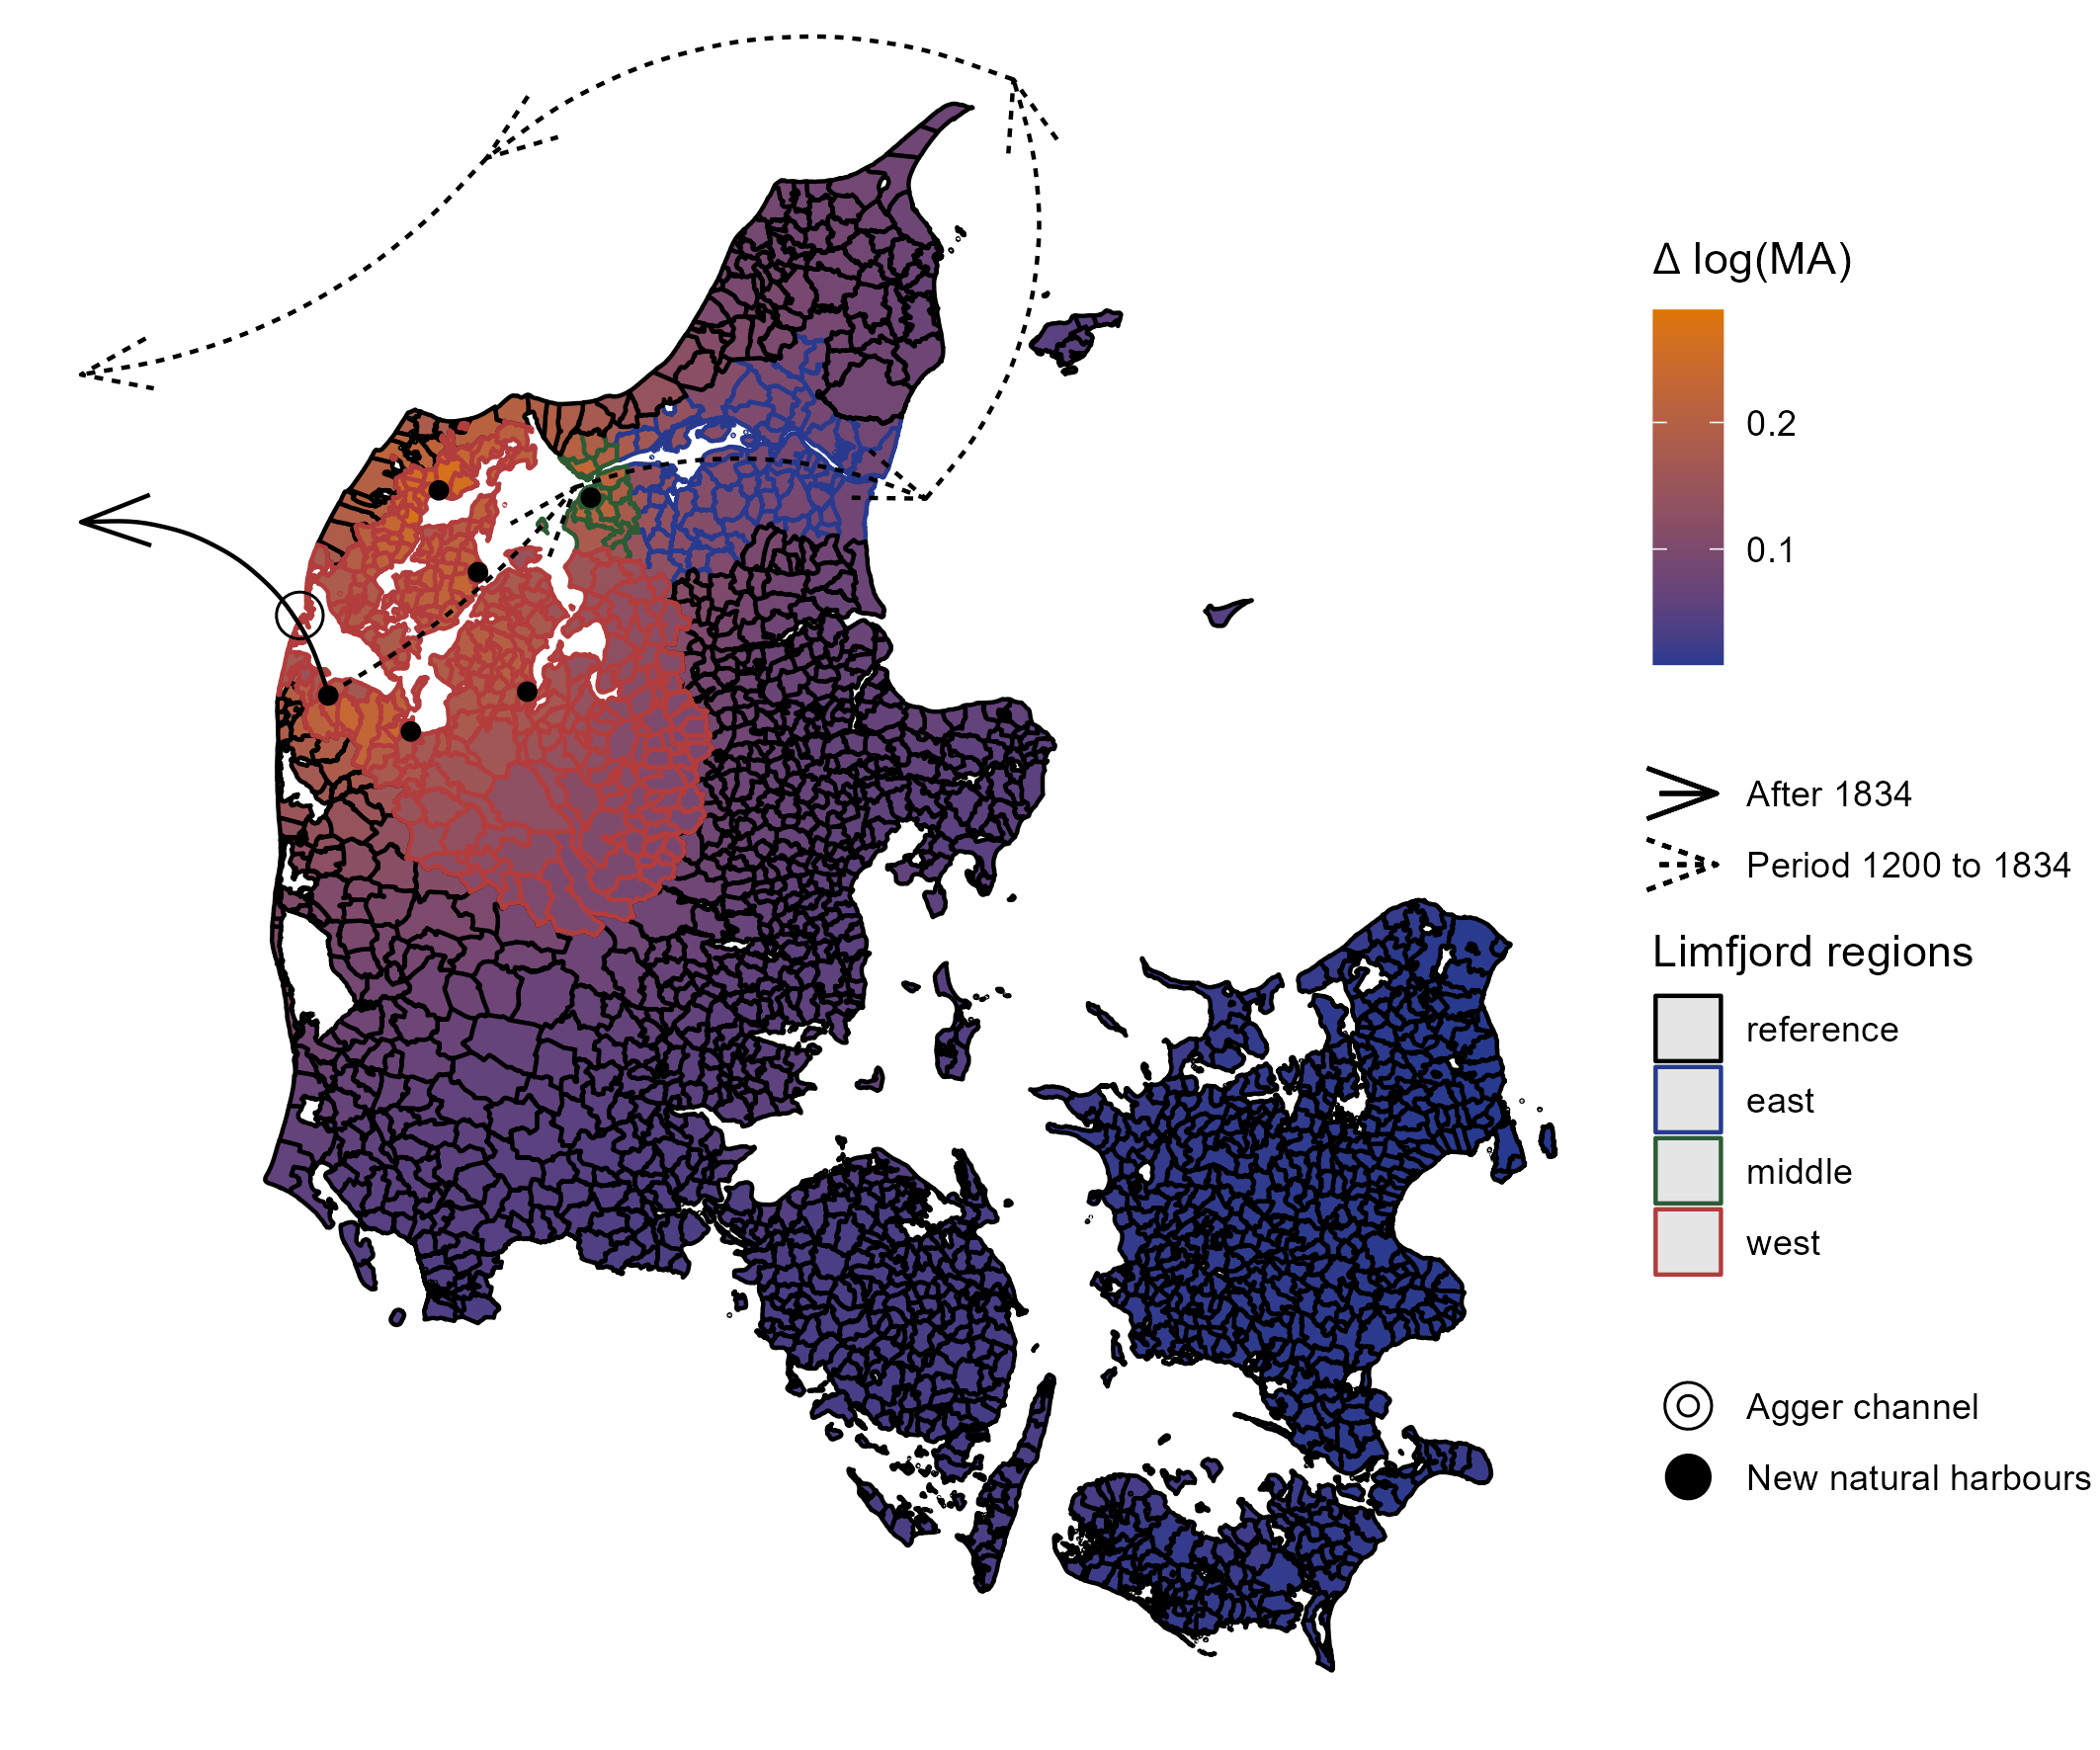
\includegraphics[width=0.8\textwidth]{Plots/Map.png}
\parbox{0.9\textwidth}{
\caption*{\footnotesize \textit{Notes:} The effect of the 1825 Agger Isthmus breach on shipping routes. The map shows improved market access (fill color) and Limfjord regions (border color). The arrows indicate shipping routes before (dashed) and after (solid) the breach. \\ \textit{Source:} Parish borders from www.digdag.dk}
}
\label{fig:main_map}
\end{figure}

\section{Introduction}
In the broadest sense, there are two types of long-run explanations for why some places prosper while others struggle: Institutions \citep{rodrik2004institutions} and geography \citep{Henderson2018satelite}. A predominant consensus suggests that institutions play a primary role, with geography exerting its influence through its impact on the formation of institutions \citep{Acemoglu2001, rodrik2004institutions, Easterly2003, Ketterer2018}. But even among geographical explanations, the evidence to suggest the importance of path-dependence and second-nature geography \citep{Krugman1991, Bleakley2012, Ager2020a} and relegates the role of first-nature geographical fundamentals as being merely important as seeds of future growth and development \citep{Davis2002, Bosker2017, Allen2023}. This paper demonstrates the importance of first-nature geography in its own right. This is done by using a natural experiment that suddenly changed first-nature geography. This in turn caused an increase in trade, population density, and both manufacturing and fishing: A large permanent causal effect of first-nature geography on the level and location of economic activity.  

In 1825 a violent storm breached the Agger Isthmus in Northwestern Denmark. An erosion process was initiated and in 1834 a navigable channel had formed. The isthmus had previously separated the Limfjord from the North Sea. But now the region was endowed with convenient access to the open ocean and world markets (see Figure \ref{fig:main_map}). Market towns of the West Limfjord had previously been small and isolated. Now they grew to become relatively important ports of international trade. Similarly, a channel in approximately the same location closed between 1085 and 1208. After the last ice age, Northwestern Denmark was left with a convenient westward channel, used by traders and Viking fleets alike. But it would close due to gradual land-rises - an ongoing process since the last ice age \citep{Christensen2004}. What followed was a long-run stagnation of the West Limfjord region until the geographic circumstances were reversed in 1825.

This paper provides evidence for the effects of these shocks in a difference-in-difference framework. This is done using historical census data, a large database of Northern European historical trade (the Sound Toll Register) and the densities of archaeological findings. It is shown that the 1825 breach led to an increase in population of 24 percent in 1901. To document the mechanisms, I have collected new data on all Danish occupations (13.5 million observations) in the period 1787-1901. The Danish censuses contain a description of each person's occupation. A new machine learning procedure, \textit{OccCANINE}, is applied to these descriptions to convert them into standardized HISCO codes with high accuracy \citep{leeuwen2002hisco, dahl2024breaking}. The HISCO-coded census data is then used to estimate the effect on occupational structure. The key finding is that the channel caused both fishing and manufacturing to grow. An important question is whether the improved geography caused growth or simply reallocation of prosperity. Using age, gender and birthplace information it is shown that the population growth came primarily from fertility - not migration. Denmark of the 19th century was in a post-Malthusian regime, where improved living standards cause fertility \citep{Jensen2022, Galor2011}. Taken together, the evidence of this paper suggests that intrinsic growth is the most likely explanation of the observed effect. That is, improved first-nature geography seemingly causes intrinsic growth - not just a reallocation of growth that would have occurred elsewhere.

For the 11th-century closing, the analysis relies on archaeological data and the closing of the previous channel as an exogenous shock. The time variation comes from the dating of archaeological sites. The geolocation of sites containing coins and buildings is used to construct panels of the probable location of economic activity. A branch within archaeology, Settlement Scaling Theory \citep{Ortman2020}, argues for such approaches to infer historical economic activity, and archaeological evidence has also seen recent application within economics \citep{Davis2002, Barjamovic2019, Bakker2021Phonecians, Allen2023}. In this paper, I develop a novel method to determine the probability that a coin or building finding was left for later archaeological discovery at any given time. Results show that a one percent decrease in market access led to a 13 percent decrease in the probability of coin findings being generated. Denmark of the 11th century is very different from its 19th-century counterpart. But despite differences in technology, culture, institutions, religion, and most other aspects thought important for economic development, geomorphology played a similar role in the 12th century as it did in the 19th century, providing evidence of (temporal) external validity of the effect of first-nature geography on prosperity.

A separate but related contribution of this paper is in understanding the benefits of infrastructure. Some of the most expensive and extensive projects that a society can undertake are infrastructure projects. Infrastructure changes distances between people. Infrastructure alters first-nature geography. However, infrastructure investments are often endogenous to outcomes of interest.  If a dramatic increase in e.g. population density is observed following infrastructure, it is difficult to identify whether this is because it was just constructed in an already thriving place. There are different standardized identification strategies commonly applied in the literature \citep{Redding2015}. This paper can be seen as an entirely new way of studying infrastructure change by relying on changes in the natural endowments of it.

Although events like the ones studied in this paper are rare, there are still plenty of opportunities to investigate similar phenomena in the vast expanse of history. For instance, both the histories of Bruges and Königsberg/Kaliningrad are marked by the consequences of an unstable channel \citep{Houtte1966, Charlier2011, Britannica2018}. And climate change threatens to cause many similar events as a consequence of natural disasters \citep{IPCC2022} and the melting ice might cause a new northern sea route \citep{Bekker2018NothernSeaRoute}. The approach presented in this paper offers a feasible method to extract new knowledge from these events and many others like them. This yields and enables new insights into both current and historical developments. 

This paper proceeds as follows. Section 2 outlines this paper's relation to the literature. Section 3 presents the historical background. Section 4 presents the overall empirical strategy. Section 5 presents a general overview of the data used. The remaining sections demonstrate empirical results. Section 6 demonstrates how the shock caused an increase in trade. Section 7 shows how the channel caused the population to grow. Section 8 covers mechanisms. Section 9 demonstrates the effect of the closed-up channel in the 1100s. Section 10 concludes. 

\section{Literature}

This paper enters a debate about the fundamental determinants of prosperity. Is geography or are institutions the fundamental cause? \cite{Acemoglu2001} argue that extractive institutions set up by colonizing Europeans are partially to blame for the current low-income status of many African nations. \cite{rodrik2004institutions} argue that geography plays a limited role if institutions are kept constant. \cite{Henderson2018satelite} use satellite image data to show that geography through trade and agriculture can explain 47 percent of the worldwide variation in economic activity. \cite{Ketterer2018} find that first nature does play a role but institutions are far more important even when a comparison is made within European regions. It would be natural to get the impression, that geography is simply unimportant in its own right. What I demonstrate in this paper is the contrary.  

Before introducing this in more detail, it is useful to provide some clarity regarding some terms already used and provide a simple taxonomy of geography and economics. \cite{cronon1992nature} introduced the distinction between first- and second-nature geography, where first-nature geography is everything determined independently of humans, and second-nature geography is all of the geography caused by humans and their interactions. This has since become the standard framework for understanding the interplay of economics and geography in broad terms \citep{Caruana-Galizia_Okubo_Wolf_2021}. Among first-nature geography, we can distinguish between:
\begin{enumerate}
    \item \textit{Things in/on the soil/land}: Soiltype, natural resources, rainfall, etc.
    \item \textit{Geomorphology}:\footnote{Also often called 'physical geography'. But this term is confusing. A bridge is very physical. But it is not what is meant by 'physical geography'. A land-bridge on the other hand is 'physical geography'. Using the term Geomorphology circumvents this confusion.} Waterways, lakes, mountains, etc.
\end{enumerate}

A huge literature is dedicated to second-nature geography in terms of infrastructure (covered below). Among first-nature explanations of the 'what's in the soil'-type, \cite{Nunn2011a, HeavyPlough2016, Dalgaard2020} demonstrate that variation in the productivity for food (the potato, the heavy plow, and fish stock respectively) of a particular place caused increased population density. But 'what's in/on the soil'-first-nature also affects other outcomes.  \cite{Decet2023WaterWars} show how a lack of rainfall is associated with an increased level of conflict in modern-day Africa. \cite{WinnersAndLosers2022} demonstrates how land productivity caused inequality, and \cite{clark2014} demonstrate the influence on literacy. Of course, the ground might be endowed with other determinants of growth like coal \citep{ORourkeCoal2021} or peat \citep{CoalPeatPaper}. 

On the other hand, first-nature \textit{geomorphology} explanations are more sparsely covered with \cite{Diamond1997, Allen2023, Matranga2024} - all related to the neolithic revolution and the emergence of the first civilizations - as the most notable exceptions. Furthermore \cite{Henderson2018satelite} and \cite{Bosker2017} demonstrate that \textit{geomorphology} is correlated with prosperity. Of course, this is often based on the comparison between places with and without certain geomorphological features, which makes the causality contingent on the degree to which you can trust their method for controlling other differences between these places. Achieving a clean identification remains a formidable challenge. Consequently, a survey by \cite{Bosker2022} calls for the exploration of natural experiments to gain insights into the causal effects of first-nature \textit{geomorphology} on population growth. The present paper tries to fill that gap.

All of this is related to a central result by \cite{Davis2002}: Even very large disruptions of city populations (the bombs over Hiroshima and Nagasaki at the end of WWII) do not change the long-run outcomes. \cite{Brakman2004Bombs} replicate a similar result for the bombing campaigns in Germany. This result has two types of potentially overlapping explanations: It is either because \textit{first-nature geography} is the \textit{fundamental} determinant of city population for a given state of the economy, or it is because of path dependence.\footnote{\cite{CraftsWolf2014} shows a case for this: Cotton mills grew where the first-nature geography, in the form of available water power, was prevalent. When this was replaced with steam power, the location was persistent due to an interaction of first and second-nature geography - some first-nature geography (water access) is useful for both water power and steam-powered mills and the investments in buildings and surrounding infrastructure (second-nature), might as well be made to good use rather than reallocating it.} In both cases, city sizes will tend to gravitate towards their long-run trend despite disruptions. But it is hard to disentangle the causes. However, if the location of prosperity is fundamentally determined by first-nature geography, then a shock to this should have a permanent rather than temporary effect. This is what I demonstrate: First-nature geography does indeed have a permanent impact on the location of prosperity. 

That is not to say, that path dependence does not play a role. \cite{Bleakley2012} convincingly document a case of path dependence. Places that used to be in favorable geography continued to be urban centers even when the geographical features that made them so became irrelevant. An implication of \cite{Krugman1991} is that small initial first-nature geographical differences can accumulate into very different outcomes via second-nature geographical interactions \citep{Caruana-Galizia_Okubo_Wolf_2021}, which is consistent with the observation of \cite{Bleakley2012}. The present paper documents fairly large and permanent effects within a generation when first nature changes, which firmly demonstrates an important role of the \textit{first-nature fundamentals} explanation of the location of economic activity. When favorable geomorphology in the Limfjord region deteriorated, so did the local economy, and when it reverted 700 years later, the economy (and population) increased dramatically. It is not \textit{just} path dependence.\footnote{Two more related publications are \cite{Ager2020a} and \cite{Cermeno2019}. \cite{Ager2020a} show how a natural disaster can change relative city sizes. And on the other hand \cite{Cermeno2019} show that institutions can create towns in otherwise unfavorable geography.}

The central natural experiment used in this paper is related to \citep{Seror2020Random}. He uses the randomly altered courses of the Yellow River in China to measure the effects of waterways on population growth. The paper finds that market access led to increased population, increased taxes, and in turn reallocation of elites - presumably to avoid the taxes. \citep{Allen2023} uses river shifts and archaeological data in what is today Iraq to demonstrate that river shifts are associated with state formation. In comparison to these two papers, the relatively rich Danish data and the unique natural experiment, allow us to exploit both the 11th- and 19th-century effects of the same event, and especially the 19th-century data, combined with detailed historical accounts, makes it possible to explore mechanisms. 

Geomorphology affects market access. That is the fundamental mechanism here. As such, we can also compare the present paper to the literature on market access and infrastructure. Infrastructure is second-nature geography, but a special case: It is a deliberate change of the first-nature \textit{geomorphology}. Railways, roads, bridges, canals - even the internet - all change the effective distance between people, which used to be different because of the geomorphology. In general, a large number of papers show how infrastructure shapes everything from land value, health, industrialization, manufacturing and the persistent location of modern-day economic activity \citep{Donaldson2016, Berger2017, Berger2019a, Hornbeck2019, Bogart2019, Zimran2020a, Bogart2022, Hornbeck2024, Hornung2015}. Of course, a central worry is the endogeneity of infrastructure. Infrastructure is often built because a place is already prospering or the opposite: Because prosperity is desired. In either case, this selection on the expected growth trajectory causes bias. \cite{Redding2015} classify identification strategies for the effect of infrastructure into three broad classes: Planned routes instruments \citep{BaumSnow2007}, historical routes instruments \citep{Duranton2012} or inconsequential units instruments \citep{Berger2017}. The present paper is an innovation in this regard as a \textit{fourth} approach: The emergence of natural infrastructure.

The search for time-variation in effective distances is also motivated by the simultaneity of trade and income. If there is trade, then there is growth (in theory) and if there is growth, then this also promotes trade. As a result, there has been discussions on the relationship between trade and growth at least since \cite{ricardo1817principles}. This paper builds on a strand of this debate arising from \cite{Frankel1999}. The insight of \cite{Frankel1999} is that geography (distances specifically) is the source of variation in trade. Using changes in trade predicted by distances can then be used to estimate this otherwise simultaneous relationship. \cite{Rodriguez2001} caution that distance between countries is correlated with other things, which also determine growth, e.g. distance to the equator, institutions, etc. When this is taken into account it is no longer possible to demonstrate an effect. Yet the work of \cite{Frankel1999} still stands as an important inspiration, which motivates the seemingly paradoxical hunt for time variation in distances. The present paper is one such case of time variation in distances.

Using time-variation in distances is also the approach of \cite{Feyrer2021} who uses the closing of the Suez Canal in 1967-1975 to show that pair-wise distances between countries affect trade and trade affects income. \cite{Maurer2008} estimate the social savings introduced by the Panama Canal in the tradition of \cite{Fogel1964}. \cite{rauch2022a} measured the increased market access from the Panama Canal and use this to measure the elasticity of market access to population growth. \cite{Bakker2021Phonecians} demonstrate that trade-inducing geography even in the time of the Phoenicians seemingly caused prosperity as measured by the density of archaeological findings. 

In the interpretation of results, I rely on the theoretical nexus between population growth and economic growth in Malthusian and post-Malthusian economies, which is well accounted for in Unified Growth Theory \citep{Galor2005, Galor2011}. Importantly, evidence suggests, that Denmark was in a post-Malthusian regime in the 19th century. This implies, that a positive shock to productivity will cause both raised living standards and higher population density \citep{Jensen2022, Klemp2016}. And this is indeed what the present work demonstrates to be the effect of improved market access. 

\section{Historical background}
A fjord is a navigable inlet of water - typically found in Northern Europe and in particular Scandinavia. Fjords act as important natural infrastructure by connecting otherwise remote regions with convenient waterways. The word 'fjord' takes its origin in the Proto-Indo-European 'pertu-', which evolved into many of the words describing roads, access points, or infrastructure more broadly. E.g. 'pertu-' is also the origin 'port', 'per' as in per capita \citep{EtymFjord}. This demonstrates how fjords even in prehistory were perceived as important, primarily in terms of their transportation capabilities. The fjords acted as the Scandinavian highways in a time before modern transportation systems. Looking at a map, it is noticeable that many Scandinavian towns and cities, even today, are located on the shore of a fjord.\footnote{Stockholm, Oslo, Gothenburg, Bergen, Stavanger, Odense, Aalborg and Roskilde just to name a few important cities from around Scandinavia, which fit this description.}

The story of the present paper is centered on the so-called Lim-fjord, named after the high concentration of subterranean lime \citep{lexlimfjord2017}. It is located in Northwestern Denmark, more specifically the Northern part of Jutland (the peninsula 'jutting' out of Germany). The region is located conveniently at the heart of Scandinavia, between modern-day Norway and Sweden. Before the 1100s, the Limfjord had both an eastern and a western opening, making it a safer shortcut for ships wanting to avoid the rough sea of Skagerak - the strait between Norway and Denmark. It is no surprise that the Limfjord developed into the main hub for Vikings to gather before sailing west to trade (and pillage) \citep{Rasmussen1966}. In the center of the Limfjord, the settlement of Aggersborg grew large and would become the location of the largest of a series of so-called ring castles constructed in the 10th century when the Jelling dynasty (of which Harald Bluetooth is probably the most well-known) consolidated power over an emerging Danish state \citep{pedersen2014}. But this would not last: The western opening would close and the local economy would stagnate, as shown by the analysis of the present paper.

The last historical evidence of the use of a western opening was in 1085. King Canute IV gathered his fleet in the Limfjord, to sail west and uphold his ‘claim’ to the English throne after his great uncle Canute II ('the great') who had been King of the so-called North Sea empire consisting of England, Denmark, Norway and parts of Sweden \citep{Spejlborg2012}. The sailors and soldiers rebelled against Canute IV, the fleet never left Denmark and he was killed when seeking refuge in Saint Alban’s church in the town of Odense in 1085.\footnote{The very place where I wrote this paper.} He was later sainted for this and earned the nickname ‘the holy’ \citep{Pajung2012}. This event marks the last attempt at gathering a Viking fleet in Denmark to sail west. Never again would Vikings be able to use the western channel. Never again would Danish Vikings try to conquer England \citep{Roesdahl2009}.

The next time this channel shows up in history is in the writings of the early historian Saxo \cite{saxo}. Saxo reports in the past tense that there 'used to' be a convenient Western channel.\footnote{\cite{saxo} book XIII, section 5} There is some uncertainty surrounding the timing of the writings of Saxo. But it is known that it was around the year 1200, and the historian, \cite{Mortensen2018}, notes that the year 1208 is most likely. Therefore, it can be determined that the western channel probably closed sometime between 1085 and 1208. This approximate timing is supported by geological surveys. By drilling through the layers of soil and deposits, geologists have demonstrated a change in the levels of salinity consistent with a closing channel around this time \citep{Christensen2004}.

What followed was no less than a complete reorientation of the prosperity of the Limfjord region. The Eastern Limfjord – particularly the town of Aalborg - became an important center of the herring trade between Hanseatic Lübeck and the rest of the Baltic \citep{sildeboom2022}. By the earliest counts of market town populations in 1672, Aalborg had become the largest Danish market town after the capital, Copenhagen. The Western Limfjord towns lagged far behind the Eastern Limfjord \citep{Degn1989}. The regional socio-economic and legal structure that developed would mirror the geography. The west coast was dangerous, difficult, and costly for ships to approach \citep[p. 176]{Hald1833}. In practice, Western Limfjord market towns mainly accessed the market by traveling eastwards through the difficult-to-navigate waters of Løgstør in the middle Limfjord and then further on through the town of Aalborg (see Figure \ref{fig:main_map}). In several court cases in the 16th and 17th centuries, the Western Limfjord market towns fought (unsuccessfully) for the right to trade independently of the whims of the Aalborg merchants \citep[pp. 78-89]{ThistedLokalhistorie1974}, but the geography made it difficult. Ships would have to pass both Løgstør and Aalborg and only limited trade occurred \citep{Poulsen2019}.

It is important to note that there was \textit{some} trade to and from the region via the west coast. But this was under direct or indirect Aalborg authority. Only small boats could directly approach Jutland's west coast beach (under perilous danger). But this was enough for a small consistent trade between Norway and the Western Limfjord to be sustained. \cite[p. 30]{Aagard1802} reports that Thisted (in the west Limfjord) shipped off 6993 barrels of barley and 6832 barrels of oats in 1800. Of this 31 percent and 47 percent respectively were shipped directly from the dangerous west coast beaches, whereas the rest was shipped via Aalborg. Of this, we can assume that most went to Norway. In return, Norway would then ship timber to the region used for construction \citep[p. 234]{Christensen1735}. However, this isolation would not persist.

On the night between February 3rd and 4th, 1825, a storm flooded the narrow strip of land called 'Agger tange' (Agger Isthmus). The Agger Isthmus was located in a remote corner of the Limfjord and was sparsely populated. The few inhabitants (388 in the 1801 census) of the Agger parish were offered money to relocate to less dangerous places to live. Many of them settled further into the Limfjord \citep{Poulsen2019, Poulsen2022}. The more remarkable effect was that on the local geography. The Limfjord and the North Sea were now connected. The geographical morphology had changed fundamentally. Shrubs and other plant material protecting the eroding coast were washed away and a shallow Agger channel had formed.

The main effects of the breach happened in three stages. \textit{First} there was a windfall gain in fish caught within the Limfjord (1825-1828) after which fishing within the Limfjord stagnated, while open ocean fishing grew. \textit{Secondly} the channel became navigable and caused a large influx of trade (1834-). \textit{Thirdly} the influx of trade caused institutions and secondary infrastructure to adapt, which boosted local prosperity even more (1840-).\footnote{For a thorough historiographical account see \cite{Poulsen2022}.}

As for the \textit{first effect}, the breach caused the salinity of the water to change and thus the fish (that otherwise had lived in brackish waters) fled. In this process, they were easy to catch and a few 'golden years' of fishing followed \citep{Poulsen2007}. This peaked around 1828, and what followed was a period of very low yields. Several species went extinct or near extinct \citep{Poulsen2019} and local fishermen had to adapt to fishing for other species in the open ocean instead of the fjord. Whether the benefit of trade outweighs the loss of food, was a topic of discussion even in contemporary times \citep[p. 1]{petersen1853oplysende}. However, the results presented in the present work indicate that it was on average a benefit.

The \textit{second effect} was the increase in trade of the region. In 1834 ships started consistently travelling through the channel. Already in 1831, experiments were conducted. But it would not be until later, in 1834 that ships would pass consistently. The simple before/after impact on trade was large. The data from the sound toll register is used to document this econometrically later in this paper, but for now, it is also useful to note that some indicative direct but scattered quantitative evidence exists for this in the historical sources. Taking the case of the market town of Thisted, (after the channel) ideally located in the West Limfjord: In 1834, 6 ships were registered in the Thisted port, while in 1876 the same number was 62. The impact in terms of products traded was also large. In 1853 Thisted exported 24735 barrels of barley and 68091 barrels of oats \citep[p. 153-159]{ThistedLokalhistorie1974}. Comparing these figures, to those reported by \cite{Aagard1802} in 1800 (mentioned earlier), this is an increase of 354 and 997 percent respectively. For the entire Limfjord, the effect was also substantial. In 1835, 19 ships used the Agger channel and in 1855 almost 2000 ships used the channel \citep{Svalgaard1977}. Newspapers report of ships arriving from England from 1834 and forward with things like coal \citep{ThistedAmtsavis1834, RoskildeAmt1836, ViborgStift1852}. This has led historians to conclude that a golden age of trade in the region had begun \citep{Poulsen2019, Ravn1993}. It quickly became the job of someone to count and register ships that passed the channel. Figure \ref{fig:channel} shows the remarkable growth in traffic as reported from this \citep{Svalgaard1977}.


\begin{figure}
\begin{center}
  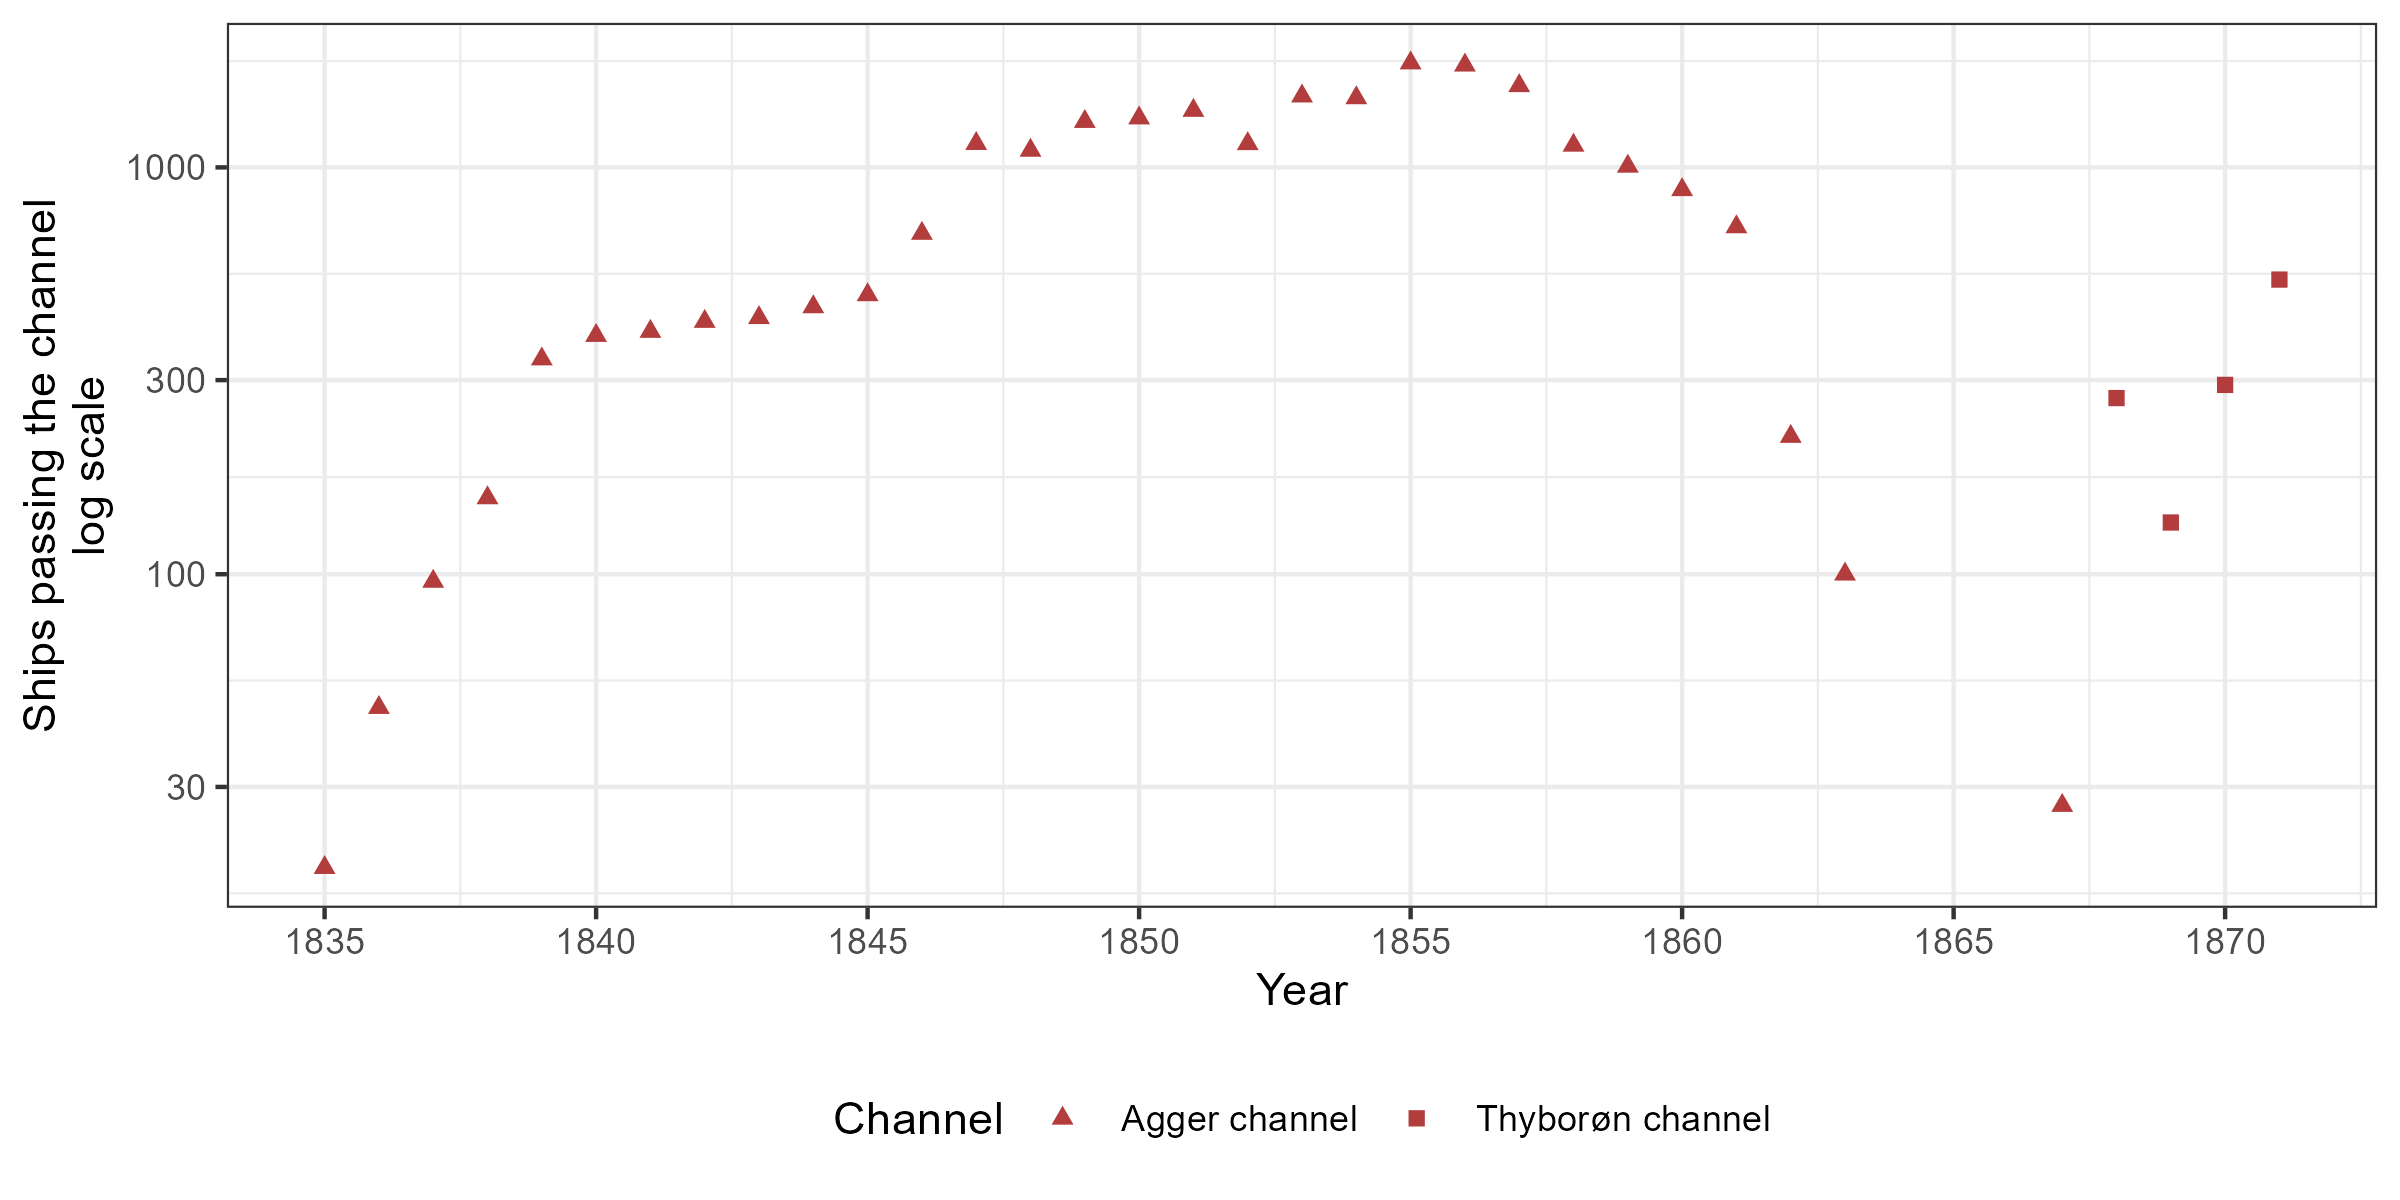
\includegraphics[width=1\textwidth]{Plots/Ship_trafic_channel.png}
  \caption{Number of ships passing the Agger channel} \label{fig:channel}
  \parbox{0.9\textwidth}{
    \caption*{\footnotesize \textit{Notes:} This shows the number of ships passing the Agger channel and later Thyborøn channel. \\ \textit{Source: Svalgaard (1977). The observation from 1867 is from Ravn (1993).}}
  }  
\end{center}
\end{figure}

The \textit{third effect} was a process of institutional adaptation and more infrastructure construction to accommodate this new trade-economy. \cite{Redding2015} argue that an initial infrastructure investment might attract even more infrastructure to accommodate the growth. They argue that this will inflate the initial effect of infrastructure investment and this might be the reason why the empirical papers find a larger effect of infrastructure than theoretical predictions. This is exactly what happened in this case. In 1841, the King granted international trading rights — independent of Aalborg — to all the Limfjord market towns. In practice, this meant customs offices in all these market towns. Previously, only Aalborg had a customs office. We can speculate that this was a matter of practicality given the new geography. With all the trade now coming through the Agger channel, it seemed self-defeating to maintain the administration of all the trade in Aalborg. The traffic itself was also a logistical problem for the ports. The market towns on the Limfjord coast only had very limited ports, and capacity was overwhelmed. This attracted investment in a series of new ports.\footnote{Thisted got a port in 1841 \citep[p. 384-386]{Dioerup1842Thisted}; Struer got a port in 1856 which was further expanded in 1864 \citep[vol V, p. 467]{Trap3}; In 1857 a port was constructed in Lemvig \citep[vol V, p. 474]{Trap3}; Nykøbing Mors had a port from 1788, but in 1843 it was purchased by the city to support trade \citep[vol IV, p. 214]{Trap3}; Løgstør had a port from 1820 but it was expanded in 1852 \citep[vol IV, pp. 399-400]{Trap3}}.

Another large infrastructure investment, the Frederik VII canal (1861), was attracted because of fears that the Agger channel would silt up. The sand would travel with the currents, and only a true local would know exactly when and where to approach the channel with ships. The depth of the Agger channel varied a lot. In 1845 it was 5 feet deep - in 1846 it was 9½ feet deep \citep{Petersen1877} and the traffic passing would vary together with this. Around 2000 ships used the channel in 1855. In 1867 it was only 28 \citep{Ravn1993}. Political pressure arose to permanently improve connectivity and market access within the region \citep{petersen1853oplysende}. For the time and the technology, this seemed most practical to achieve by doing something for the connection between the East and West Limfjord at Løgstør. At first, attempts were made in 1843 at clearing the silt out of the shallow waters of Løgstør \citep[p. 311][p. 4]{Bergsoee1844, petersen1853oplysende}. This would fail and eventually, a more expensive but feasible solution was found. It was decided to build a canal along the coast near Løgstør to circumvent these waters.

A part of the story of adaptation also revolves around the introduction of steamships. In 1842 a permanent route by steam was established between Aalborg and Copenhagen and soon after the towns of the Limfjord were also interconnected via steamships \citep{Klem1967}. Steamships would be the vessel for the future important butter trade with origin in Esbjerg \citep{Lampe2015DanesUK}, but the first attempt at establishing a Danish route - the steamship "Jylland" - took its origin in the Limfjord and the Agger channel \citep[p. 62]{Schovelin1891}. However, by then the Agger channel had become more shallow and this put a natural limit on the size of the ship, which merely had a draught of five feet \citep{Lassen1883}. The Agger channel, would eventually completely silt up, but before this happened another channel (approximately in the same location) would open in 1867 \citep{Petersen1877}. This channel - called the Thyborøn channel - still exists today.

The problems with the navigability of the West Limfjord channels probably contributed to the choice of Esbjerg as the location of a large port for Danish/British trade - rather than somewhere in the Limfjord. After the success of artificially establishing a safe port in Esbjerg \citep{Lampe2015DanesUK}, and due to increasing concerns that the Thyborøn channel would also silt up, it was decided to establish a series of groins along the northwestern coast of Denmark in 1875. This final bit of adaptation would protect the area from coastal erosion and secure the existence of a western channel of the Limfjord to this day.

\section{Empirical Strategy}
This paper identifies three main effects: The effect of the channel on population size, the effect of the channel on trade, and the effect when a similar channel closed in the 1100s on economic activity. However, the empirical strategy is similar across all. The events used here are by themselves isolated exogenous shocks limited to a specific time and a specific region. The effect of the channel can therefore simply be computed as the change in an outcome in the areas affected by the channel compared to the areas not affected by it. This generally takes the form of a classical event-study specification.

\begin{equation}
\label{eq:eq501}
\log(y_{it})= \alpha_t + \alpha_i + \sum_{j=1787}^{1901} 1[t=j]Affected_{i}\beta_{j} + \varepsilon_{it}.
\end{equation}

Here $y_{it}$ is the outcome of interest (e.g. population) in a parish $i$ at time $t$. $t=1801$ is used as the reference. $1[t=j]$ is an indicator taking the value 1, when $t=j$ and zero otherwise. $Affected_{i}$ measures how much parish $i$ was affected by the new channel. Therefore $\beta_j$ represents the time-varying effect of being affected by the channel. That is, how much larger is e.g. log(Population) in affected parishes than in non-affected parishes when the general population trends and initial sizes have been accounted for? Whether a specific parish is affected by the channel is measured in two distinct ways, one is atheoretical and based on a simple dummy, and another is inspired by theory and based on estimates of how the channel affected local market access. On one hand, it is beneficial to have a simple binary measure for locations affected or not affected. On the other hand, it is probably not realistic that the effect is homogeneous across various locations. However, modeling this requires assumptions on the spatial pattern of the effect of the channel. This motivates the use of both.

The dummy measure of being affected is constructed by a simple heuristic of categorizing parishes into different parts of the Limfjord. This is used in the following regression setup: 

\begin{equation}
\label{eq:eq502}
\begin{split}
\log(y_{it})= \alpha_t + \alpha_i + \sum_{j=1787}^{1901} 1[t=j] \times 1[i\in west]\beta_{j,w} + \sum_{j=1787}^{1901} 1[t=j] \times 1[i\in middle]\beta_{j,m} \\
+ \sum_{j=1787}^{1901} 1[t=j] \times 1[i\in east]\beta_{j,e} + \varepsilon_{it}.
\end{split}
\end{equation}

The region directly affected by the channel is the West Limfjord (see historical background) while the Middle and Eastern Limfjord were affected indirectly. For this reason, the parameters of interest are the $\beta_{j,w}$'s, which measures the average change in the outcome in logs - approximate percentages for small values. Parishes are categorized as being 'Limfjord' parishes if they are closer to the Limfjord than any coast. The West and East Limfjord were separated by difficult-to-navigate waters at Løgstør (see historical background). A roughly northwest, southeast line going through Løgstør is defined by the coordinates (57.044185, 9.186837) and (56.958951, 9.275585). This separates the eastern and western Limfjord in a conventional sense. A buffer zone of 20 km around this line is defined as the 'middle' Limfjord. Any parish west of this buffer zone is categorized as 'west' and any parish east of this is categorized as 'east'. Figure \ref{fig:main_map} illustrates all of this information.

Estimates of Market Access are motivated by the spatial heterogeneous effect of the channel. Some parishes had more benefit than others since they were closer (in cost distance) to the new waterway. The effect of the change in Market Access is estimated and used in the following regression setup: 

\begin{equation}
\label{eq:eq503}
\log(y_{it})= \alpha_t + \alpha_i + \sum_{j=1787}^{1901} 1[t=j] \times \Delta log(MA_i)\beta_{j} + \varepsilon_{it}.
\end{equation}

Here $\Delta log(MA_i) = log(MA_{i,after}) - log(MA_{i,before})$ is the change in log market access as defined below. The parameters of interest are the $\beta_{j}$'s, which measure the elasticity of the outcome to market access.  Market Access is computed based on the cost distance approach following \cite{rauch2022a} and inspired by a vast literature using similar methods \citep{Harris1954, Redding2008, Ahlfeldt2015, Donaldson2016}. The change in market access comes from the change in the set of effective ports. After the 1834 channel opened, the West and Middle Limfjord became viable ports for international cargo. 

The measure of change in market access is inspired by the process described in the historical background. Suddenly the west Limfjord ports became coastal. And this change is what I aim to pick up. The Sound Toll Register contains ports used for international cargo trade. Most of these are coastal market towns. Most trade went via the coastal market towns simply because it was legally required to do so \cite{Degn1989}. Goods would be produced in the countryside and carried to the local market town to be sold. Constructing any measures of this process requires a sensible reduction of all cost distances between $H$ ports and $P$ parishes. In this regard, Tobler's first law of geography is useful: \textit{"Everything is related to everything else, but near things are more related than distant things."} - \cite{Tobler1970}. Estimating the Market Access is one solution to this problem, which is theoretically motivated \citep{eaton2002}, follows Tobler's law and has seen wide empirical use. In this setting, the most useful property of this approach is that for every location, it returns a single number, which expresses how close that location is to all other locations. Market access is computed as:

\begin{equation}
\label{eq:MA2}
{MA}_p = \sum_{h \in H} [CostDist(p, h; \alpha) + 1]^\theta
\end{equation}

Here $H$ is the set of all available ports (H for harbour). $h$ is a specific port location and $p$ is a specific parish centroid. $CostDist(p, h; \alpha)$ is the relative cost of travelling from parish $p$ to port $h$ given the parameter $\alpha$ (defined below). 

The core aim of this entire exercise is to gain insights into how this measure changes with the breach. That is, the aim is to estimate two quantities: a) ${MA}_p|No\:channel$ b) ${MA}_p|channel$. Quite simply, this comes from the change in the set of available ports $H\rightarrow H^*$. $H$ is all the consistently available ports before 1834. $H^*$ is those consistently available after 1834 as a consequence of the Agger Channel. The estimated conditional market access can then be expressed as

\begin{equation}
\label{eq:MA3}
\begin{split}
{MA}_{p}|\textit{No channel} &= {MA}_{p}|H \\
{MA}_{p}|\textit{Channel} &= {MA}_{p}|H^*.
\end{split}
\end{equation}

Here $H$ contains all ports observed in the Sound Toll Register more than once but leaving out the ports in the Middle and West Limfjord. $H^*$ includes these. To be accurate, these ports existed both before and after. But before the breach, they saw only limited use. As this paper documents this dramatically changed with the introduction of the channel. What ${MA}_{p}|channel$ measures is the market access after the five Limfjord ports become suitable for international cargo because of the channel. $\theta$ is the distance elasticity, which in the default specification is assumed to be -1 as in \cite{Harris1954} and \cite{rauch2022a}. CostDistance is computed based on $\alpha = 10$. That is, it is 10 times as costly to travel over land than sea. Additional details are described in Appendix A. The map in Figure \ref{fig:main_map} shows the change in Market Access across Denmark given the newly available ports following the breach.

\FloatBarrier
\section{Data}
For detailed trade data, the analysis relies on the Sound Toll Registers from Elsinore (of Shakespeare's \textit{Hamlet} fame), north of Copenhagen. Denmark taxed ships passing through from 1420 to 1857 and thorough accounts were kept of all ships (1.8 million in total) \citep{gobel2010oresundstolden}. This was digitized by \cite{soundtoll_data} and their team. This data contains information on the origin and destination of each ship. Conveniently, these ports have even been labeled with coordinates. A total of 126 ports in present-day Denmark are reported in the period 1750-1855. The sum of traffic to and from these ports is used as a measure of the level of trade to and from that destination. 

Census data was obtained from Link Lives \citep{mathiesen2022linklives}. For the purposes here, it contains individual-level information such as occupation, age, gender, and the parish of residence. In the main analysis, it is aggregated into parish-level population counts. Data is available for 1787, 1801, 1834, 1840, 1845, 1860, 1880 and 1901. I manually made a crosswalk between the census data parish names and the historical parish borders (which is available in this project's public repository). Only parishes that are consistently observed throughout all the censuses were used. This leaves 1589 of 1783 parishes that were used in the analysis. 

This census data is also used to test plausible mechanisms. This is done using age, place of birth, gender, and occupation. All of the occupational descriptions in the census were transcribed into HISCO codes using \textit{OccCANINE} described by \cite{dahl2024breaking}. The HISCO-coded census data is publicly available from \cite{dk_hisco_data}. The census data contains an occupational description for each person such as "he is a fisherman and a farmer". For the years 1787, 1801, 1845 and 1880 these already had HISCO codes assigned to them \citep{ddd_method2015}. This was part of the training data for \textit{OccCANINE}. 200 random HISCO codes from the algorithm were manually and diligently checked to be 94 percent accurate. 

Table \ref{tab:desc_pop} contains summary statistics for the main variables used in the analysis. 'Population' is the number of people in each parish for that year. 'HISCO Agricultural' is the count of all individuals with HISCO codes starting with 6. 'HISCO Manufacturing' is the count of all those individuals with HISCO codes starting with 7, 8, or 9. 'Born in different county' counts the number of people who were born in a different county, than where they now live. 'Child-women ratio' is the ratio of children aged between 1 and 5 to women aged between 15 and 45, which is used as an indicator of fertility. Figure \ref{fig:bal} shows the standardized distribution of all of these before the event with the obvious exception of 'Born in different county' which is only observed from 1845. From this figure, it should be noticed that there is a large overlap between variables of interest before the Agger Istmus breach. But the pre-event difference is also noticeable. This is addressed in Section 7 and Appendix D.3. 

Archaeological data is obtained from a public registry of archaeological findings. All Danish archaeological sites are registered in a publicly available database. The data is geo-referenced, categorized by type, and dated to a certain interval of years. Every coordinate was matched to a parish using the parish borders described above. The archaeological dating of the site was then used to construct a panel of economic activity. Details of this are outlined in section 9.

\begin{table}
\centering
\caption{Summary statistics for parish level census data}
\label{tab:desc_pop} 
\footnotesize
\begin{tabular}{lcccccccc}
\toprule
  & Observations & mean & sd & min & Q0.25 & median & Q0.75 & max\\
\midrule
Population & 14301 & 652.02 & 505.88 & 27.00 & 332.00 & 526.00 & 816.00 & 13087.00\\
Affected: West Limfjord & 14301 & 0.12 & 0.33 & 0.00 & 0.00 & 0.00 & 0.00 & 1.00\\
Affected: $\Delta log(MA_i)$ & 14301 & 0.07 & 0.06 & 0.01 & 0.02 & 0.05 & 0.09 & 0.27\\
HISCO Agricultural & 14301 & 181.07 & 120.03 & 0.00 & 100.00 & 152.00 & 230.00 & 1512.00\\
HISCO Manufacturing & 14301 & 65.65 & 74.77 & 0.00 & 23.00 & 46.00 & 84.00 & 2809.00\\
Born in different county & 7945 & 253.13 & 378.91 & 0.00 & 19.00 & 72.00 & 360.00 & 4299.00\\
Child-women ratio & 14274 & 0.47 & 0.11 & 0.00 & 0.40 & 0.46 & 0.53 & 1.36\\
\bottomrule
\end{tabular}
\parbox{0.9\textwidth}{
\caption*{\footnotesize \textit{Notes:} This table contains summary statistics for the variables used, which are ultimately sourced in the census data. For most variables, there are 14301 observations corresponding to 1589 parishes and 9 census years. The child-women ratio is the ratio of children age 1-5 to women of age 15-45. 27 observations are missing from this variable since no women in the the relevant age group are observed. 'Born in different county' is only observed from 1845 and forward. \\ \textit{Source: Danish census data}}
}
\end{table}

\begin{figure}
\begin{center}
  \caption{Variable distributions}
  \label{fig:bal}
  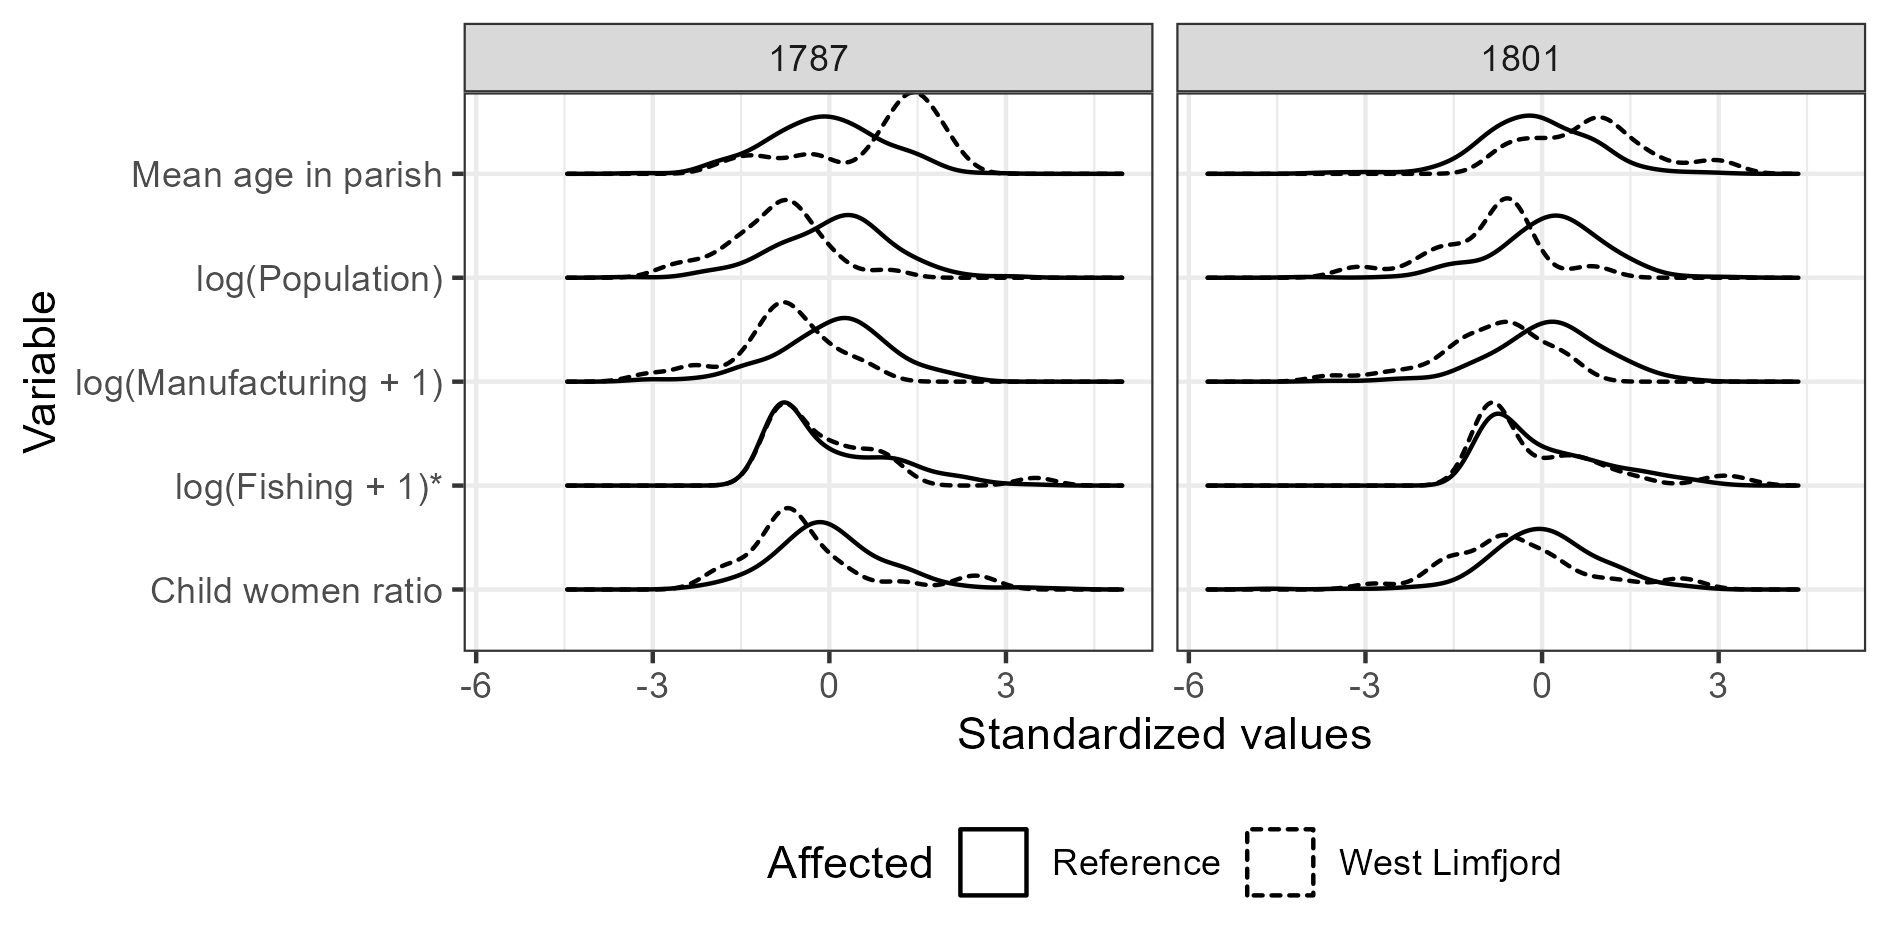
\includegraphics[width=1\textwidth]{Plots/Balancing_plot.png}
  \parbox{0.9\textwidth}{
  \caption*{\footnotesize \textit{Notes:} This shows the distribution of variables of interest before the 1825 breach in the West Limfjord and the rest of the country (excluding other Limfjord parishes). All these characteristics are broadly overlapping approximately similar, with a general trend that the West Limfjord is behind the rest of the country regarding population density and fertility. \\ \textit{Source: Danish census data}}
}
\end{center}
\end{figure}

\FloatBarrier
\section{The effect on trade}
After the Agger channel opened in 1834, there was a substantial increase in trade in the region. Figure \ref{fig:Sound_toll} shows the detailed statistics from the Sound Toll Database. This illustrates the sum of traffic to and from ports on a log scale. An important caveat is that the Sound Toll Database only counts ships that would go eastwards and pass the Sound Toll at Elsinore. However, it should be noted how practically no traffic with origin or destination in the West Limfjord is replaced by a substantial amount afterward. And this is no quirk of uncertain data. In fact, the amount of trade is relatively stable. This stability was only briefly interrupted when Denmark actively entered the Napoleonic War in 1807-1814 \citep{Feldbaek2015}. 

\begin{figure}
\begin{center}
  \caption{Number of ships to different regions of the Limfjord} \label{fig:Sound_toll}
  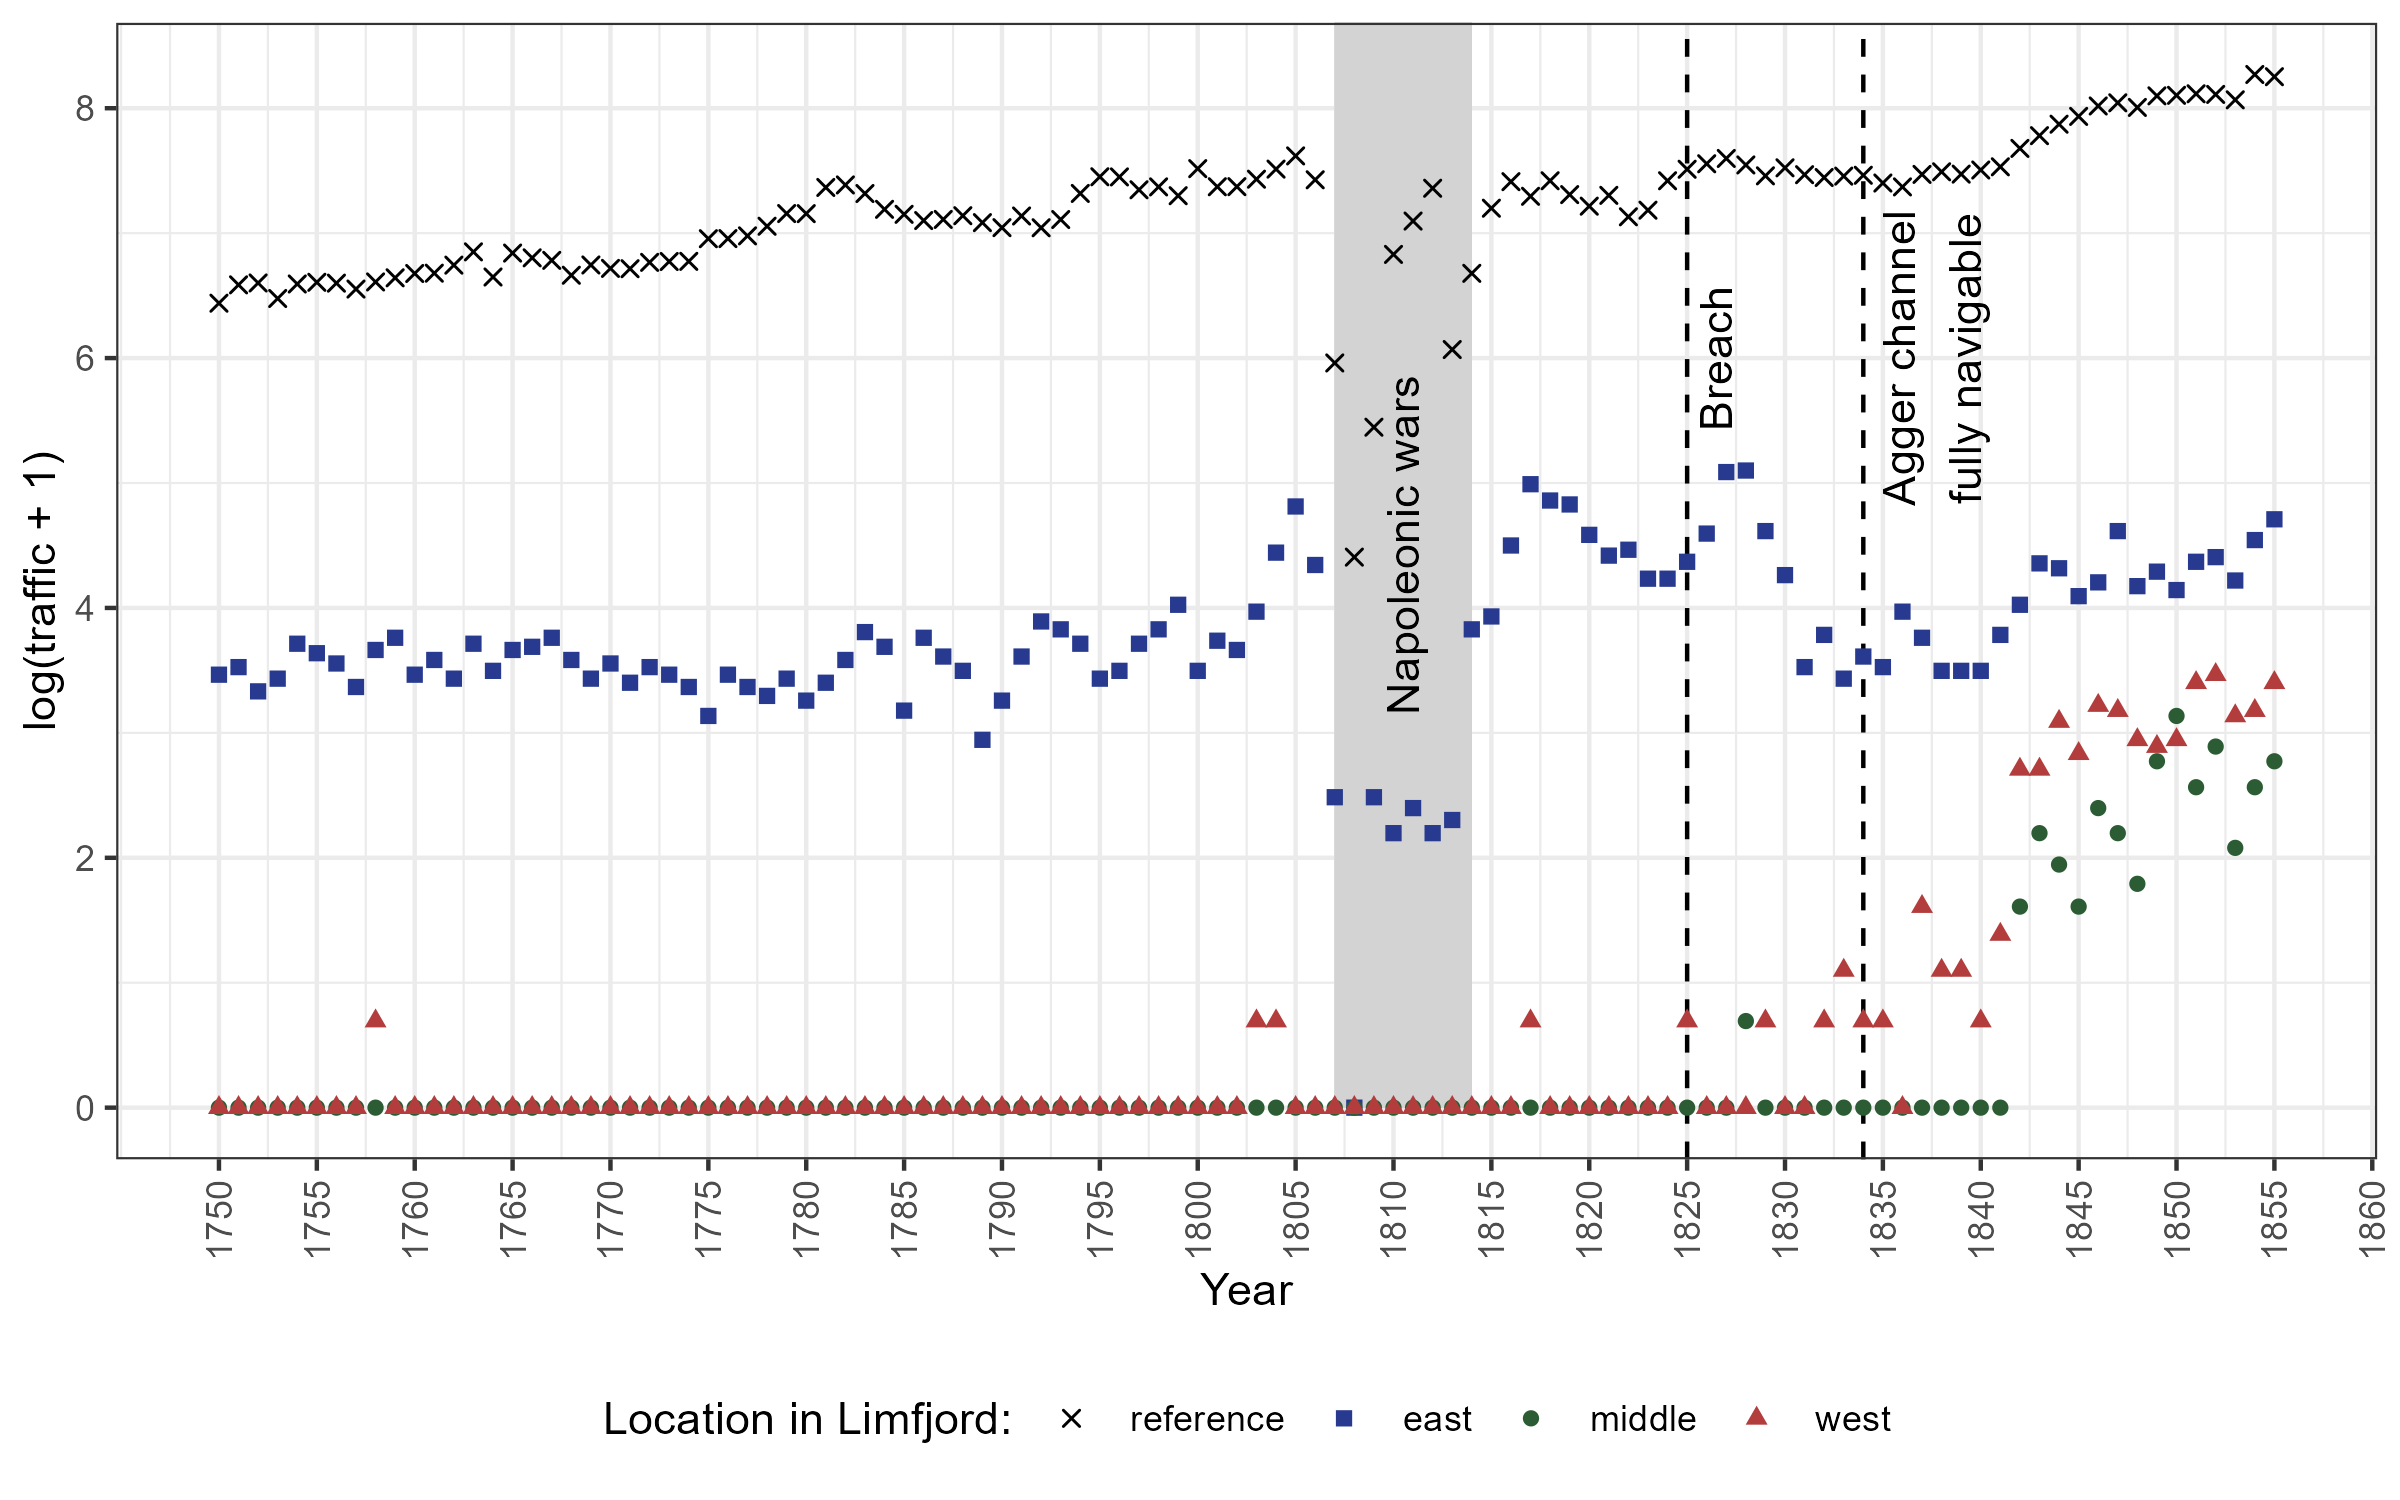
\includegraphics[width=1\textwidth]{Plots/Ship_trafic.png}
  \parbox{0.9\textwidth}{
  \caption*{\footnotesize \textit{Notes:} This shows the log-transformed sum of traffic to and from ports in Denmark as captured by those ships that passed Elsinore. \\ \textit{Source: Sound Toll Register Online.}}
}
\end{center}
\end{figure}

Figure \ref{fig:Sound_toll} (and Figure \ref{fig:channel} from Section 3) unmistakably highlights the introduction of trade to the Middle and West Limfjord following the creation of the Agger channel. While there is a certain level of traffic prior to 1834, it lacks consistency, aligning with historical sources that confirm the channel becoming fully navigable in that year. Unsurprisingly, a regression version of this (which can be found in Appendix B) shows the same result across many common specifications for this type of estimation. The analysis reveals a notable immediate, lasting surge in trade, which - according to the historical descriptions - would have placed a strain on local infrastructure, prompting further investment. First nature caused trade.

%This is a rare case, where the before/after estimate is preferable to any more advanced specification. This is because zero traffic is a very reasonable counterfactual: There would still be no shipping traffic without the channel. As such the comparison of before and after, is the most simple and reasonable estimate of the effect. This also allows us to use the full account from the channel itself. This reveals a sizeable effect. When traffic was at its maximum in the year 1855, 1805 ships used the channel. It is also seen that this traffic would diminish as the channel started silting up, but pick up again soon after, when the Thyborøn channel - in almost the same location - became navigable in 1868.

\FloatBarrier
\section{The effect to population}

\begin{figure}
    \centering
    \caption{Effect of the Agger channel on population size}
    \begin{subfigure}[b]{0.8\textwidth}
        \centering
        \caption{Dummy approach}
        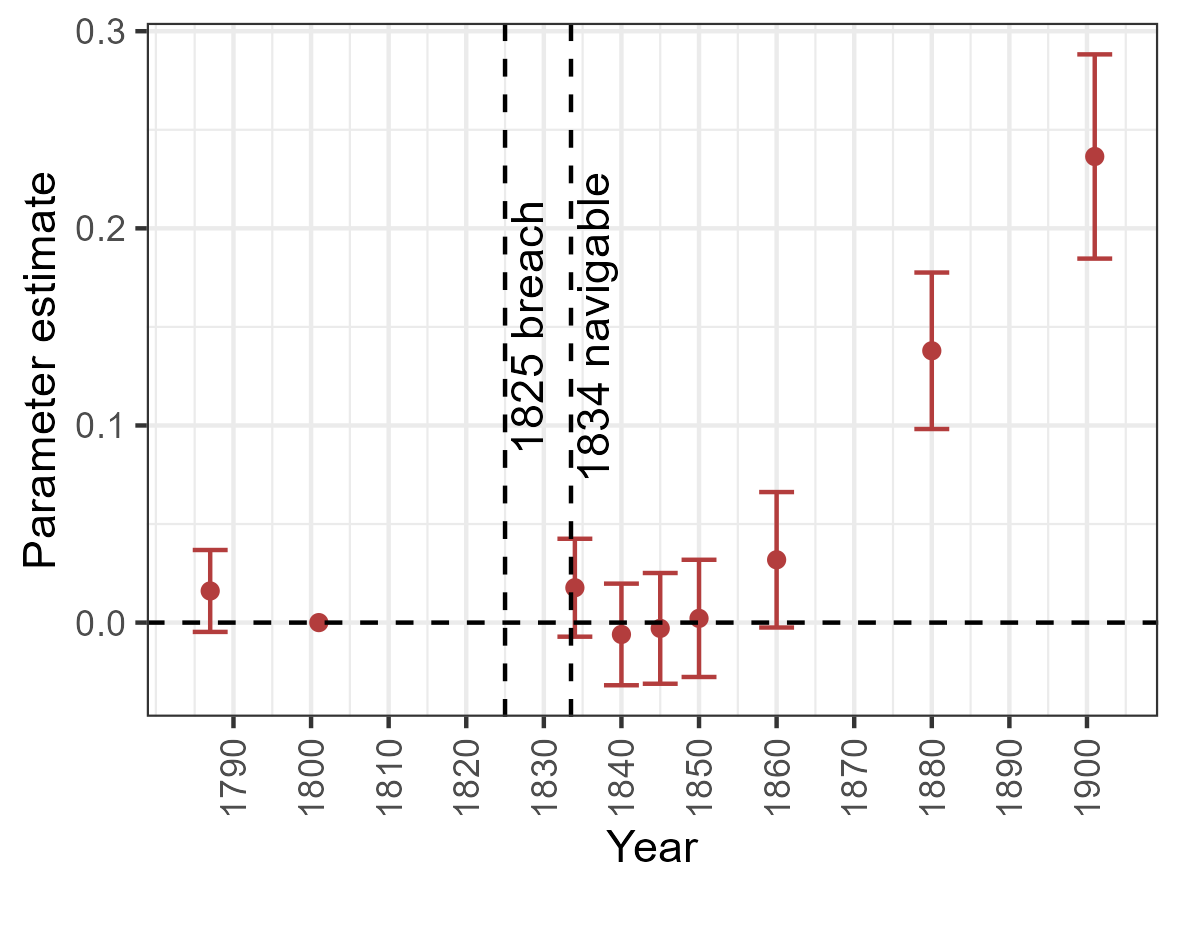
\includegraphics[width=0.7\textwidth]{Plots/Regression_plots/pop_dummy.png}
    \end{subfigure}
    \vspace{1cm}
    \begin{subfigure}[b]{0.8\textwidth}
        \centering
        \caption{Market access approach}
        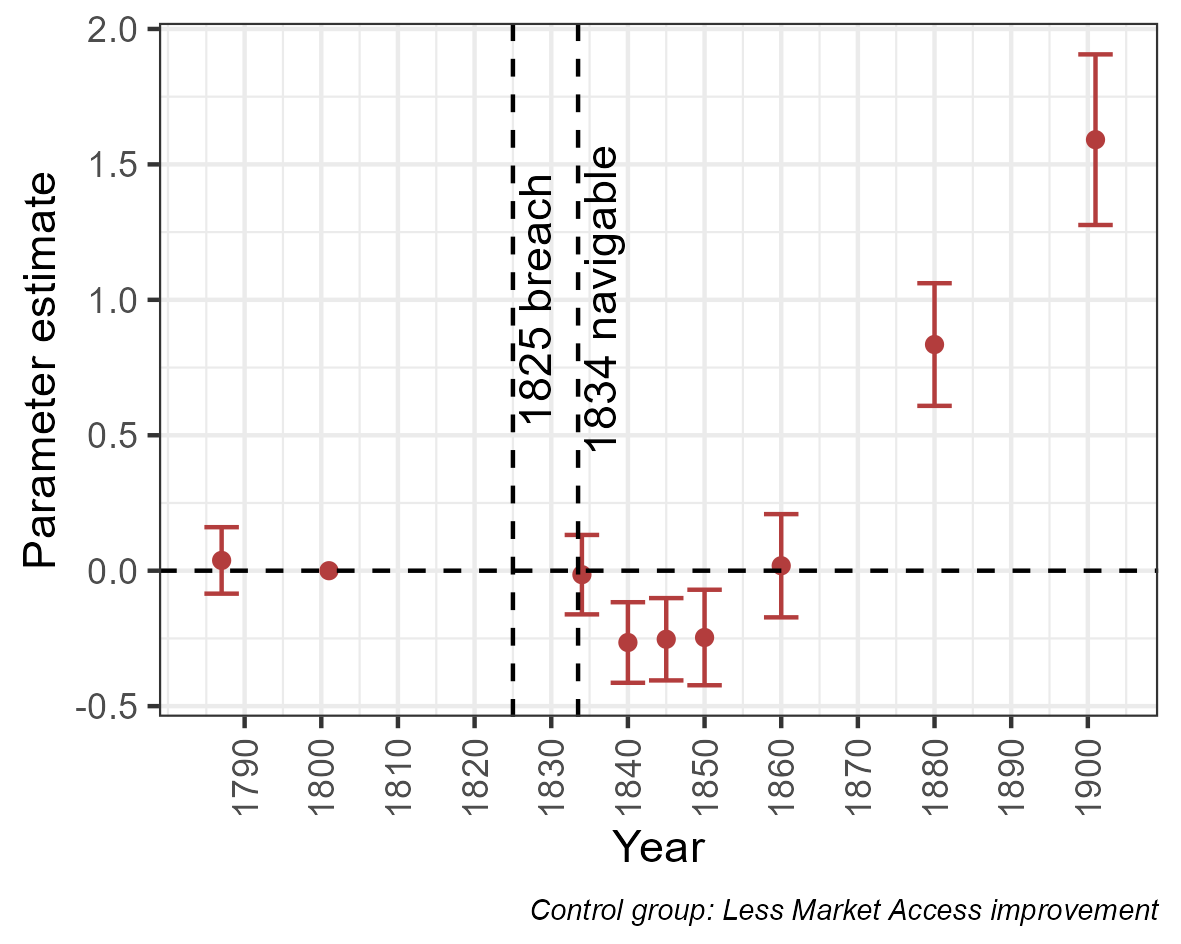
\includegraphics[width=0.7\textwidth]{Plots/Regression_plots/pop_MA.png}
    \end{subfigure}
    \parbox{1\textwidth}{
    \caption*{\footnotesize \textit{Notes:} Effect of the channel on the size of the population in the affected area. The error bars represent 95 percent confidence intervals based on cluster-robust standard errors. In the first panel, being affected is defined as a dummy for being in the West Limfjord and the second panel it is defined on the estimated improved market access from the channel. 1801 is zero because it is the reference year for both regressions. All parameter estimates can be found in appendix C.1. \\ \textit{Source: Danish census data}}
} \label{fig:pop1}
\end{figure}

The improved first-nature geography also caused the population to increase. Figure \ref{fig:pop1} shows regression results from estimating equation \ref{eq:eq501}. Panel (a) shows the simplest estimate, where being affected by the Agger channel is defined as a dummy for being in the West Limfjord. This allows parameters to be interpreted as the approximate percentage increase in the affected region caused by the channel. By 1901 the parishes of the West Limfjord region had a 23.6 percent larger population than what would have been expected by parishes from elsewhere and the population in 1801. Panel (b) shows the results when 'affected' is defined as estimated improved market access from the channel. This shows that by 1901, affected areas had experienced a population growth equivalent to an elasticity of market access of 1.59.\footnote{This is similar to the magnitude found for the Panama Canal by \cite{rauch2022a}.}

The relative delay of the effect should be noted. It is remarkable that a relatively large increase in ship traffic is not associated with any discernible effect on population size immediately. It is only by 1860, that a positive effect on the size of the affected population is observed. And for the market access approach, it even seems like there is a slight negative effect immediately after the channel became navigable. But a lot happens behind the scenes. This is addressed in Section 8. 

From Figure \ref{fig:pop1} it can be observed that there are no pre-trends in 1787. It is also possible to robustify the results against the choice of comparison group by running the same regression using a set of alternative feasible subgroups of parishes. Figure \ref{fig:pop2} in Appendix C shows exactly this. It shows the multiverse of all feasible choices of subgroups \citep{Steegen2016multiverse} for which the analysis could have been carried out, and the last panel shows all the feasible parameters for market access computation, which could have been assumed. Alternative parameters for the market access function or alternative comparison groups would all have generated positive results, leading to the same qualitative conclusion. As for pre-trends, Appendix C also contains results for the parameter for 1787. None of the alternative specification show any pretrends. Another potential worry is balance. This is addressed by correcting for pre-treatment characteristics (age, occupation, fertility) using the doubly-robust difference-in-difference estimator suggested by \cite{Callaway2021did}. The results of this are also shown in Appendix C. The effect of the channel is robust to all of this.

\FloatBarrier
\section{Mechanisms}

For population growth to occur, the people must come from somewhere. This section tests whether the observed population growth plausibly relates to higher levels of prosperity. This is done to corroborate the connection between the shock to first-nature geography and economic development. It is demonstrated that both the manufacturing and fishing industries grew, indicating that the West Limfjord fundamentally became more prosperous. Furthermore, consistent with the post-Malthusian regime of the time \citep{Jensen2022, Klemp2016}, evidence is shown that population growth is explained by fertility rather than internal migration. This also indicates that the population growth was intrinsic rather than reallocated from elsewhere.

\subsection{Occupations}
To test the impact of the occupational channel, the HISCO system's structure is utilized \citep{leeuwen2002hisco}. The first digit of each HISCO code indicates a major category of which the occupation belongs. To estimate the effect on each category, the following regression setup is used:

\begin{equation}
\label{eq:occ1}
f(y_{it})= \alpha_t + \alpha_i + \sum_{j=1787}^{1901} 1[t=j]Affected_{i}\beta_{j} + \varepsilon_{it}.
\end{equation}

Equation \ref{eq:occ1} is equivalent to equation \ref{eq:eq501} with the important difference that the outcome is not merely $log(y_{it})$ but a function $f$. Zero outcomes, which are frequent in this setting, imply a methodological trade-off between measuring the intensive and extensive margins separately or accepting that the measured coefficients are not unit-invariant \citep{roth2023loglike}. The function $f()$ addresses this issue in four distinct ways:

\begin{enumerate}
    \item Extensive: $f(y_{it}) = 1[y_{it}>0]$
    \item Intensive: $f(y_{jt}) = log(y_{jt}|y_{it}>0)$
    \item $f(y_{it}) = log(y_{it}+1)$
    \item $f(y_{it}) = arcsinh(y_{it})$
\end{enumerate}

The first function measures the extensive margin, which indicates the number of parishes that have at least one person with a specific occupation. The second function measures the intensive margin, showing the effect among parishes that already had at least one person with such an occupation. The third and fourth functions are two standard ways of measuring the combined effect, acknowledging that these estimates are not unit-invariant. 

Another concern is interpreting whether the estimates are substantial enough to explain the overall increase in population. All the transformations yield coefficients, which should be interpreted as relative effects. However, it is not particularly interesting if, for example, the number of priests increased by 50 percent from two to three. The primary focus is on whether the occupational structure shifted significantly: whether a large proportion of people adopted the professions for which the effect is tested, rather than just the relative effects. To address this, all estimates are converted to the \textit{Average Partial Effect share} ($APE\,share$), which is the average partial effect (the implied number of people gaining that occupation in an average parish), divided by the average parish size in the West Limfjord in 1901. Intuitively, this answers how large a share of a parish's population has shifted into a specific type of occupation.\footnote{Estimated from coefficients based on the formula $APE\,share_j = \overline{Occ_{j, 1901}}\beta_j / \overline{Pop_{1901}}$, where $\overline{Occ_{j, 1901}}$ is the average number of people with that profession in the West Limfjord in 1901 and $\overline{Pop_{1901}}$ is the average number of people in a West Limfjord parish in 1901. } 

Testing all seven occupational categories using both the market access and the dummy approach, and considering the four specifications of $f()$, and all of the census years involves a total of $9\times56 = 504$ separate parameters.\footnote{A back-of-the-envelope calculation would predict that 25 of these coefficients would have a p-value below 0.05, purely by random chance}. Therefore, only the parameter estimates for 1901 are presented. To address concerns over multiple testing, the Bonferroni correction is applied to the standard error of the 56 coefficients in 1901.

Figure \ref{fig:mech_occ} illustrates the Bonferoni corrected results using the Dummy approach, displaying the estimated change in a specific occupational category from 1801 to 1901 in areas affected by the Agger channel as compared to the change in the rest of the country. Each panel represents different approaches to dealing with zero outcomes, and the x-axis corresponds to the major categories in the HISCO system. The plot reveals a significant impact on the intensive margin for two particular categories: Agriculture (6) and manufacturing (7/8/9).  It is expected that with overall population growth (driven by fertility, as shown below), more individuals would enter agriculture as a default and common profession. However, these results also demonstrate a large absolute change in the occupational structure due to increased prosperity, leading to the rise of manufacturing, which was previously uncommon. Appendix D.1 includes coefficients from both the dummy and market access approach, while the event study plots from each of these estimates are available in the project's online repository.\footnote{
\url{https://github.com/christianvedels/A_perfect_storm_replication/tree/main/Plots/Mechanism/Occupations}. Note that these plots are not corrected for multiple testing. 
}

Figure \ref{fig:mech_occ2} further breaks down this effect at a more detailed level, using the first three digits of the HISCO codes for agricultural occupations and the first two digits for manufacturing occupations. Notably, the growing manufacturing occupations include those traditionally associated with industrialization, such as textile production and "workers not elsewhere classified," which encompasses generic factory workers. This suggests a fundamentally increased level of economic activity resulting from the improved first-nature geography. Regarding agricultural occupations, the growth of fishing reflects how the population benefited from the sudden availability of fish in the North Sea. 

Please note that due to the large number of regressions conducted, confidence intervals were not even estimated for Figure \ref{fig:mech_occ2} as they would be uninformative after appropriate corrections. The figures should be understood as descriptive. The development of the fishing industry was gradual, while spinning only took off between 1880 and 1901. This can be seen in event plots of these two occupations, which are included in Appendix D.2. \cite{Poulsen2007} show how an effect of the channel was a collapse of Limfjord fishing due to the increased salinity when the saline Northsea broke through. A hitherto open question is whether open ocean fishing (which the channel enabled) were able to offset this negative effect. This was indeed the case: Fishing became an approximately 15-20 percent more common profession in the area, laying the grounds for a future industry. Today, Thyborøn, located just at the mouth of the channel, is one of Denmark's main fishing ports, accounting for 25 percent of the Danish catch in 2021.\footnote{Data extracted from \cite{MinisterietforFodevarer2022}.} It is noticeable how there is essentially no development in spinning until something rapidly happens between 1880 and 1901, which is timed with the economic take-off in Denmark \citep{Khaustova2015}. Taken together, these results are evidence to suggest that the improved first-nature geography caused increased levels of economic activity as a plausible mechanism for population growth. 

\begin{figure}
\begin{center}
  \caption{Impact of the Agger Channel on Occupational Structure in 1901} \label{fig:mech_occ}
  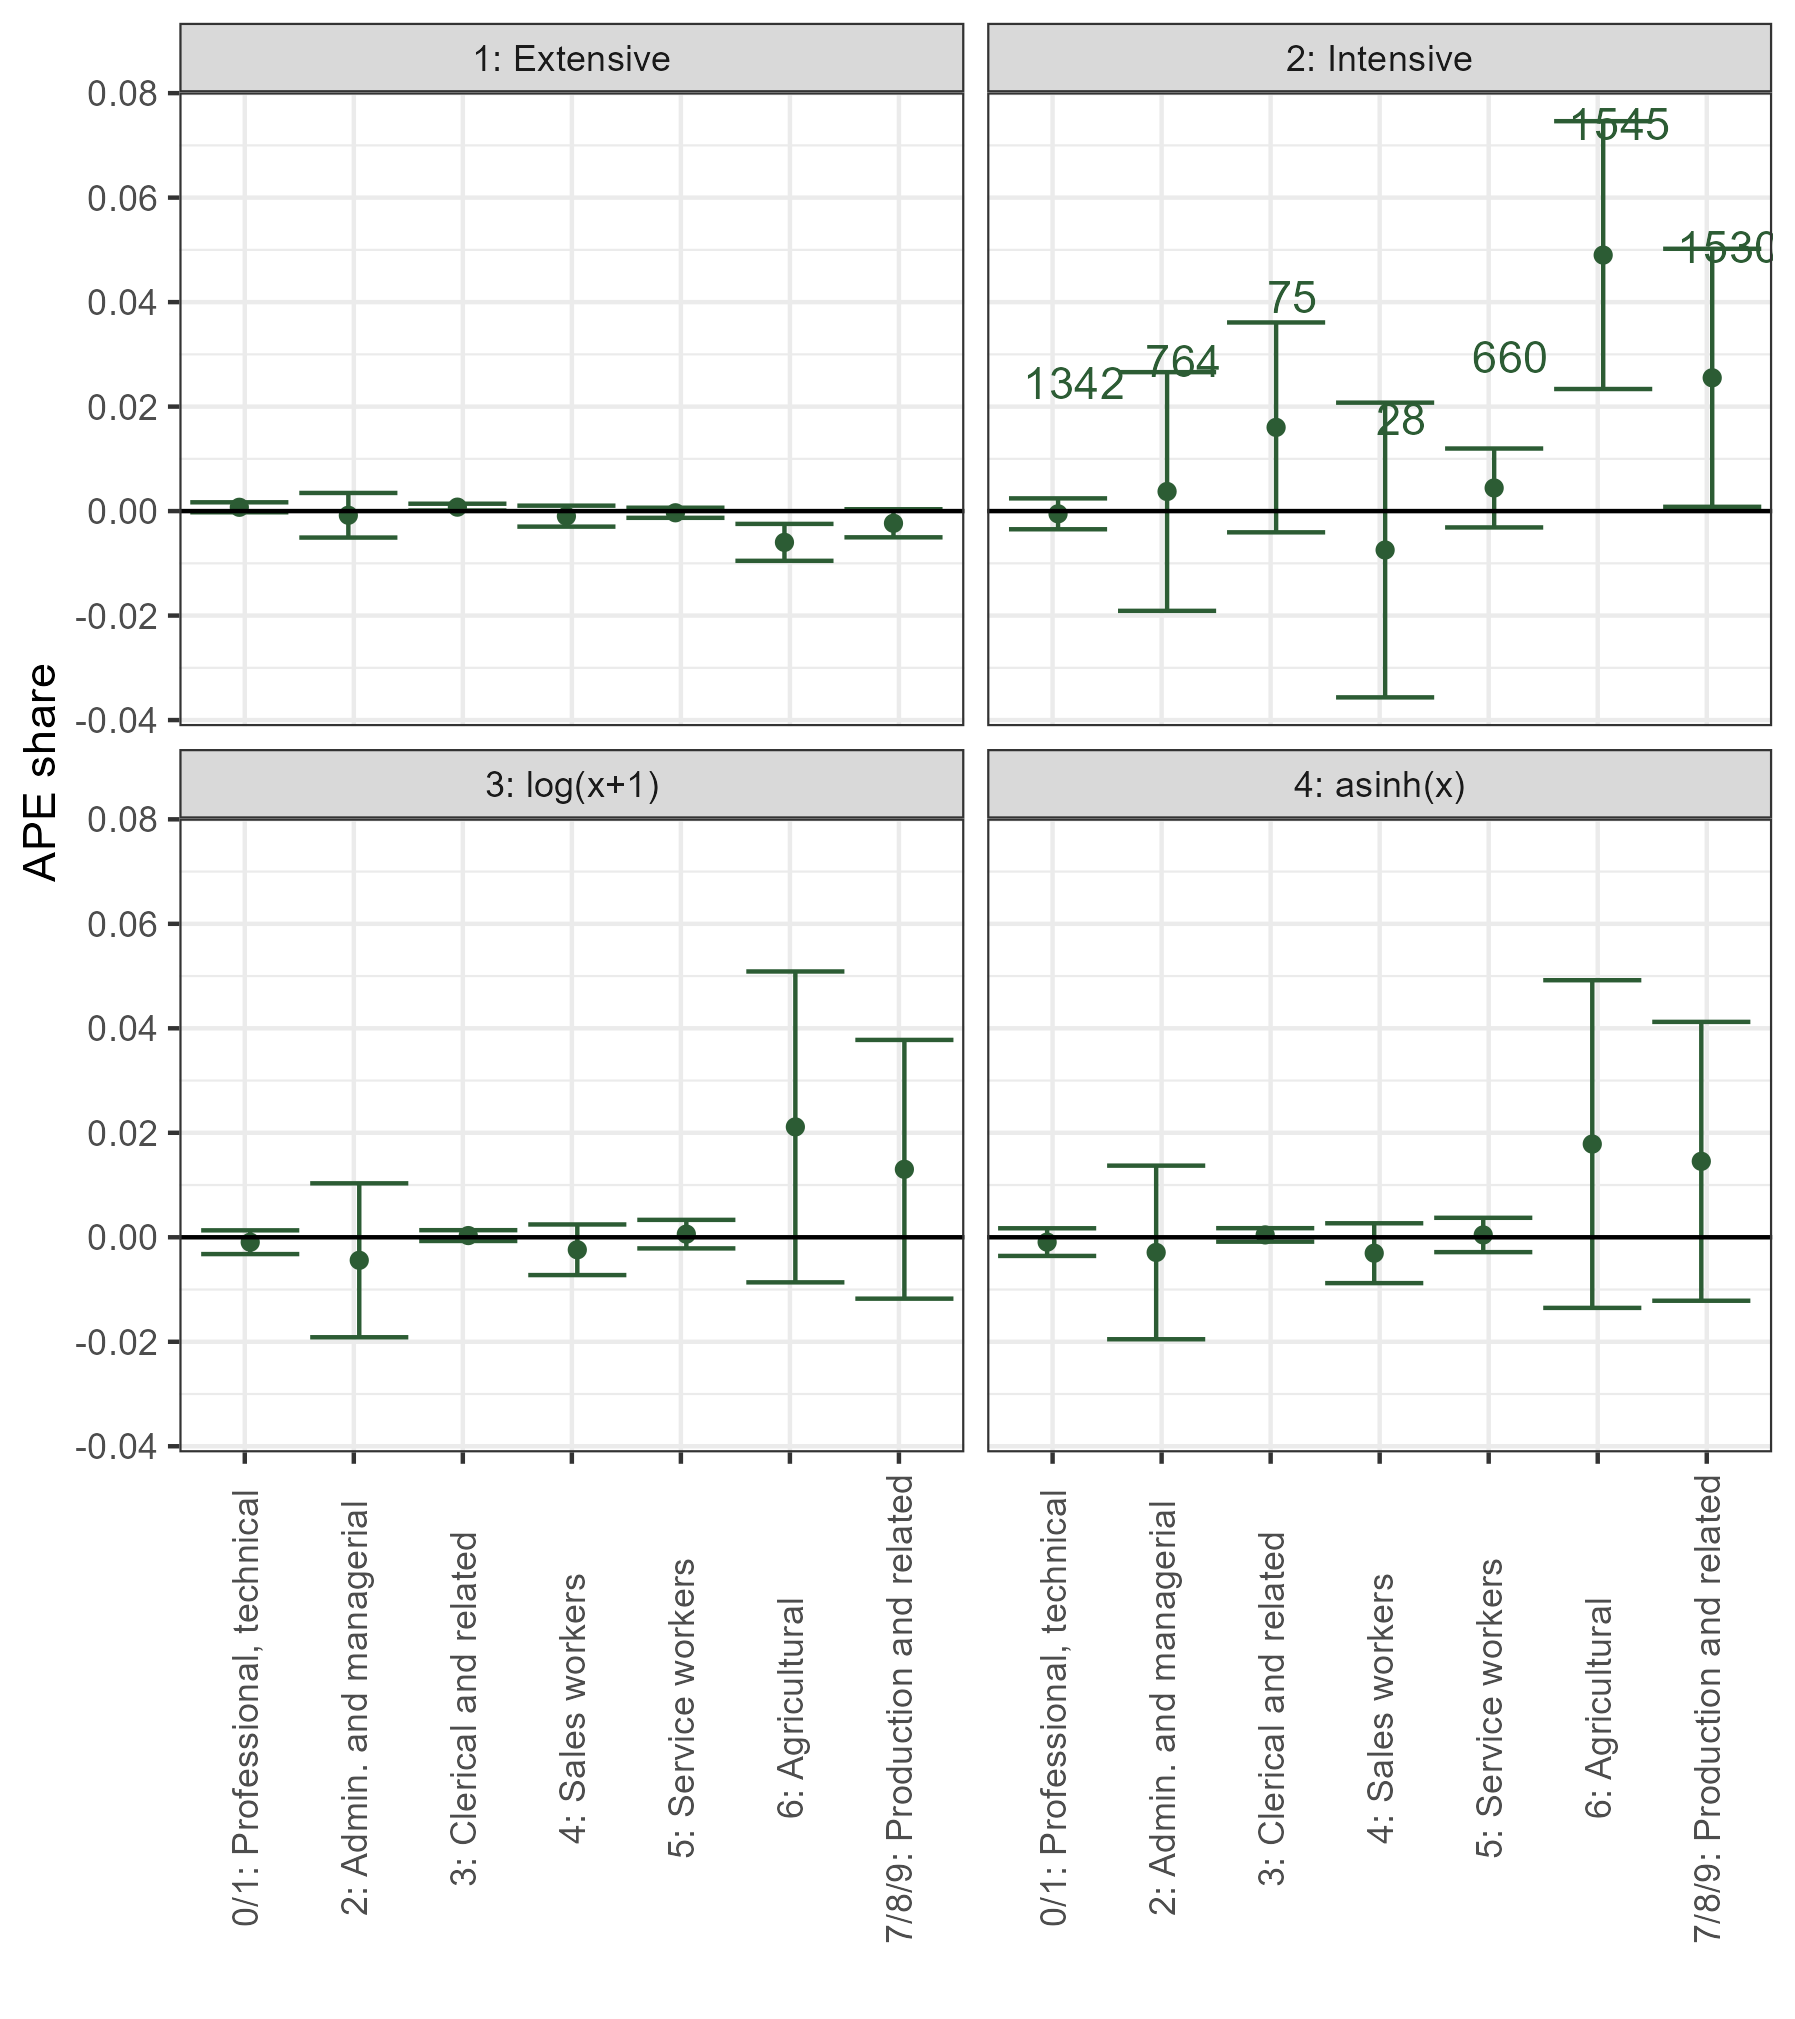
\includegraphics[width=0.8\textwidth]{Plots/Mechanism/All_occupations_dummy.png}
  \parbox{0.9\textwidth}{
  \caption*{\footnotesize \textit{Notes:} This figure illustrates the average partial effect (as a share of parish size) on the occupational structure in 1901. The first panel shows the effects on the extensive margin. The second panel shows the effect on the intensive margin (with included number of parishes shown as well). Instead of choosing between intensive and extensive margin, the third panel uses the $log(x+1)$ transformation and the fourth panel uses the inverse hyperbolic sine transformation. The results are based on the Dummy definition of being affected by then channel. Appendix D.1 shows a table of all results including results based on market access. The error bars represent 95 percent confidence intervals corrected for multiple testing using the Bonferroni correction. This is based on standard errors, which are clustered at the parish level.}
}
\end{center}
\end{figure}


\begin{figure}
\begin{center}
  \caption{Effects on Detailed Occupational Structure} \label{fig:mech_occ2}
  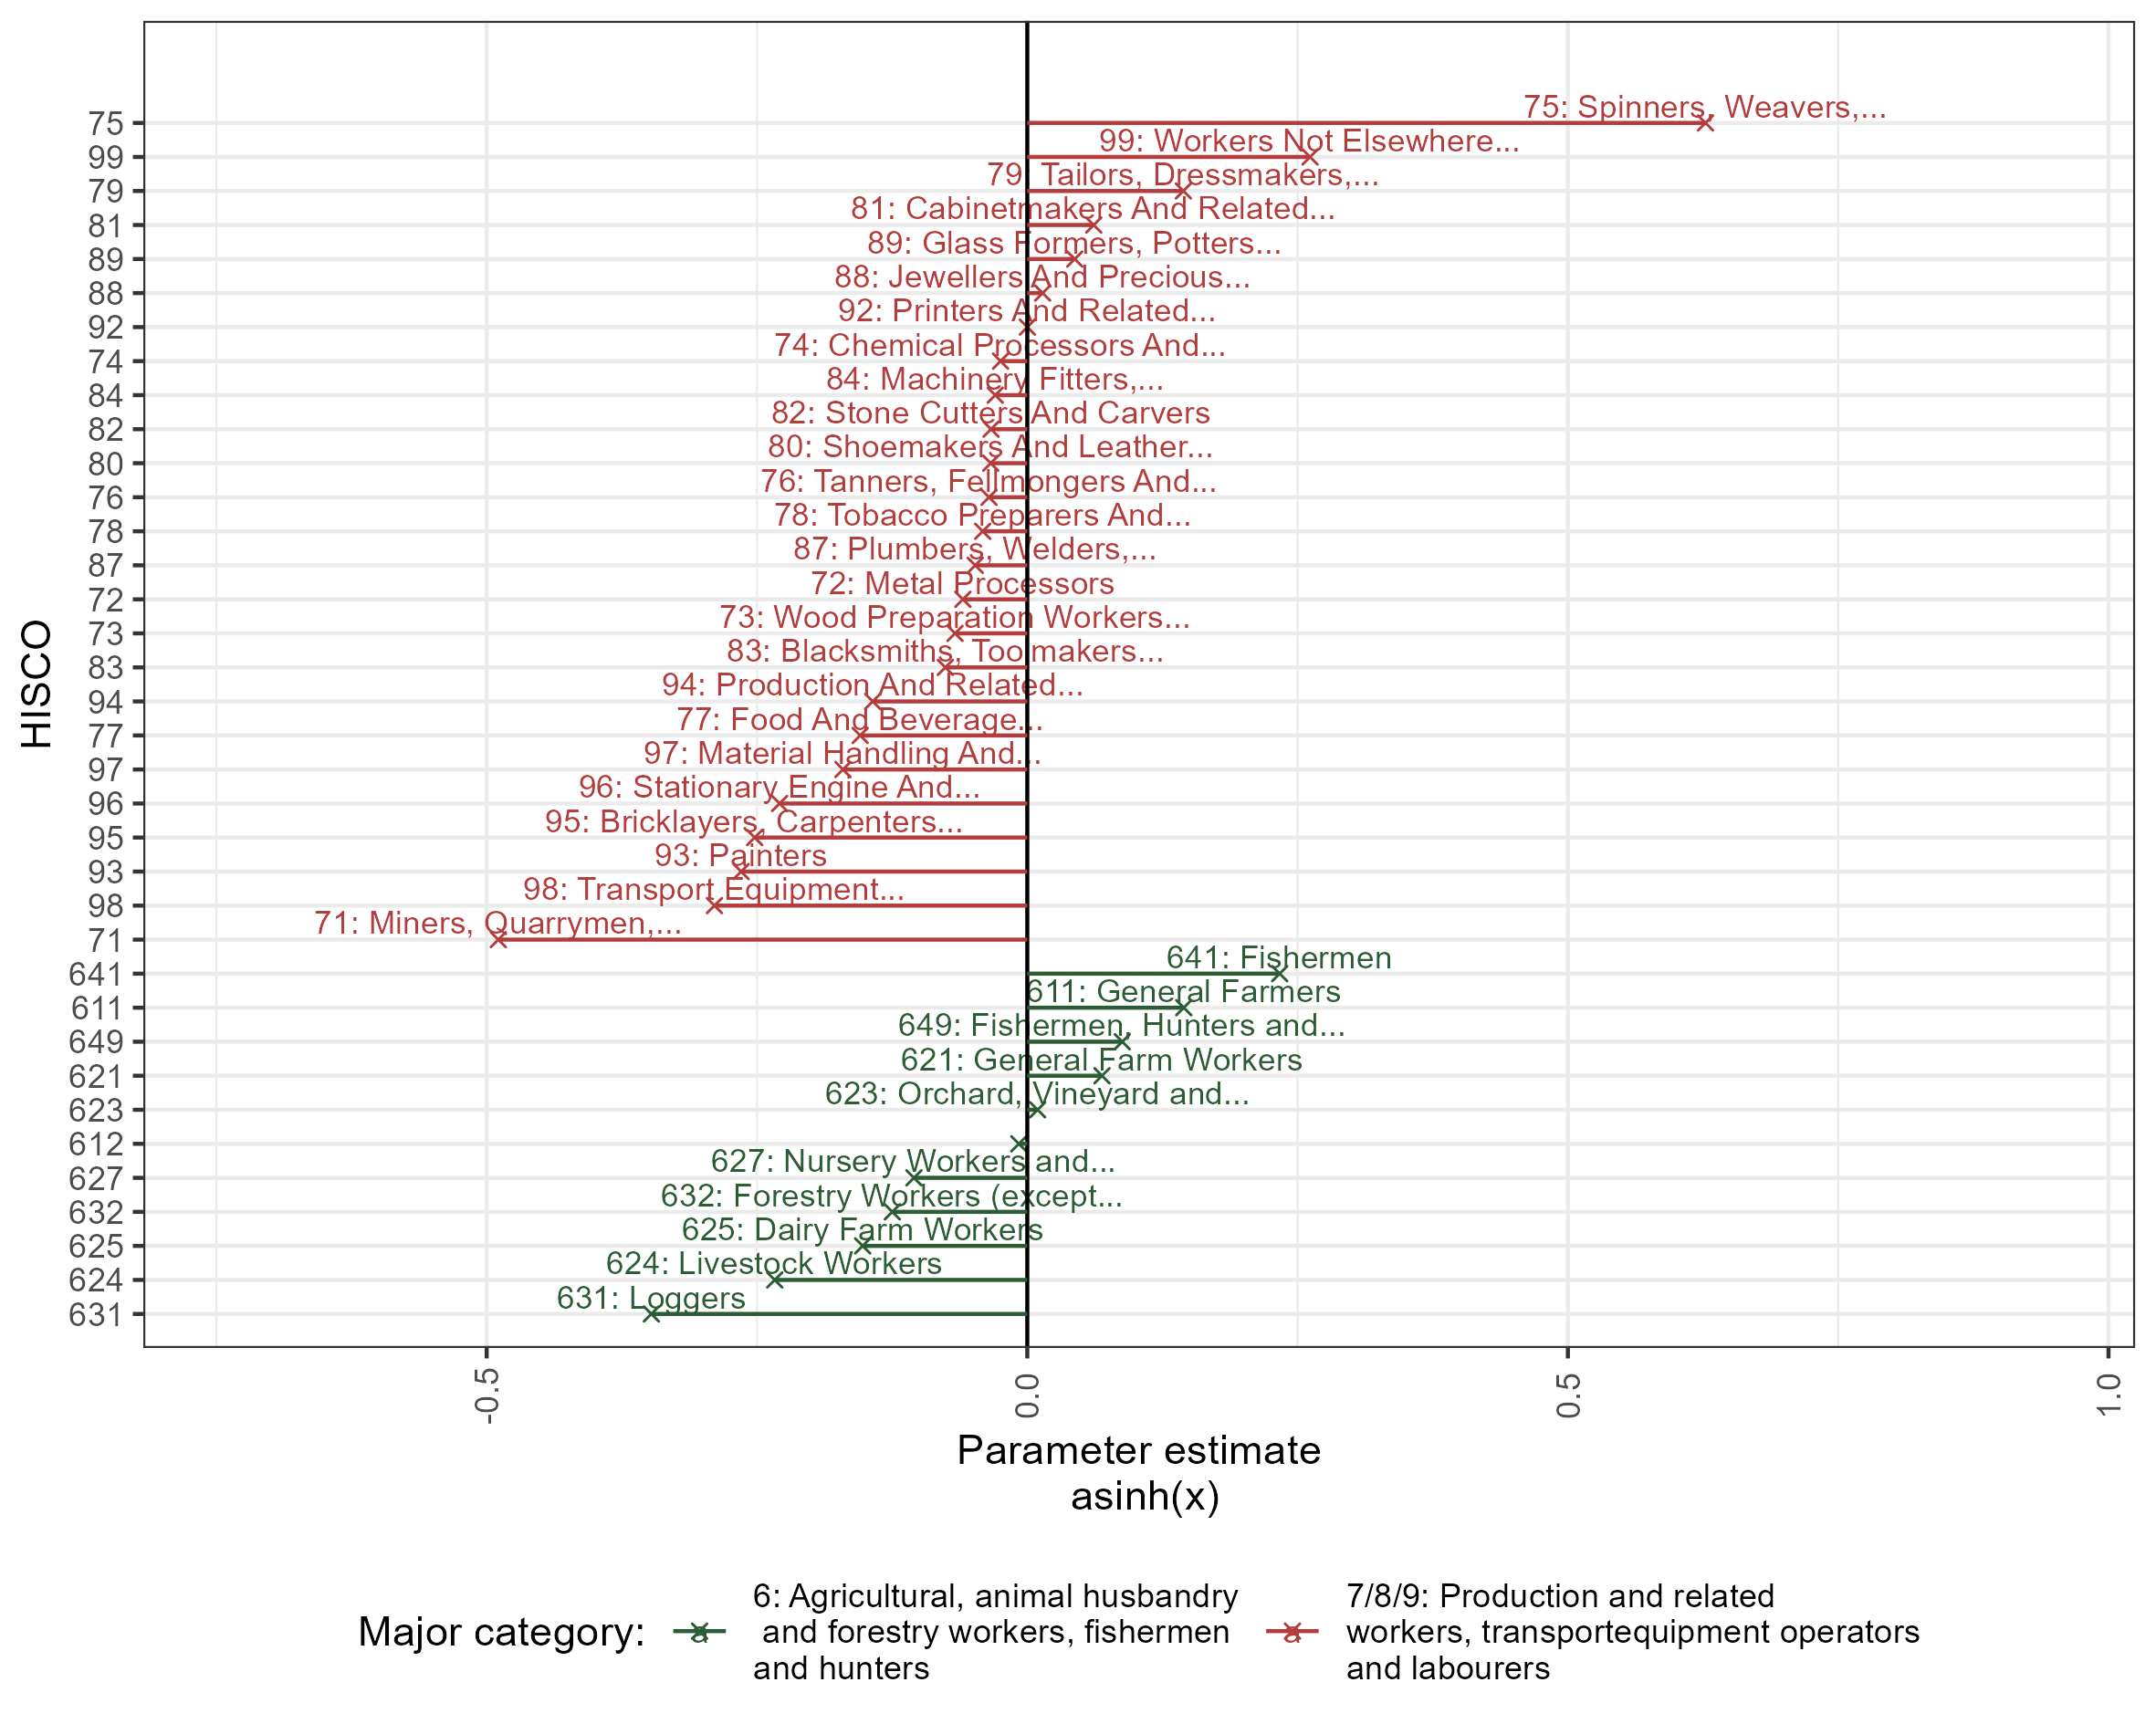
\includegraphics[width=1\textwidth]{Plots/Mechanism/Detailed6789/Dummy_asi.png}
  \parbox{0.9\textwidth}{
  \caption*{\footnotesize \textit{Notes:} This figure depicts the relative changes in subcategories of agricultural and manufacturing occupations (HISCO codes starting with 6 and 7/8/9). The plot presents the results using the arcsinh transformation and the dummy-definition of being affected by the channel. Qualitatively similar results using alternative approaches are available in online repository.}
}
\end{center}
\end{figure}

\FloatBarrier
\subsection{Fertility and migration}
A key question is whether first-nature causes growth or simply reallocates it. Indicative evidence comes from migration rates. If the channel reallocated population from elsewhere, then it should be observed in higher (internal) migration rates to the affected area from elsewhere. On the other hand, if the increase in population is more intrinsic, then given the post-Malthusian dynamics of this time \citep{Jensen2022, Klemp2016}, it is expected that increased living standards would lead to higher fertility.

Figure \ref{fig:migr_fert} shows event plots for migration and fertility rates. Migration is measured as the number of people born in another county than their current county as a share of the total population in their parish of residence. Fertility is measured as the child-women ratio. Panel (a) and panel (b) shows results for fertility. The channel resulted in 11.6 percent higher fertility in 1901 (panel b), which corresponds to 0.96 percent increase for every percent increase in market access (panel b). The results for migration indicate a negative effect or no effect depending on whether the market access approach is used (panel c) or the dummy approach is used (panel d). This indicates that observed population increase is not the consequence of migration. In fact, there was out-migration in the period, at least in terms of cost distance from the newly available ports, which is what is captured by the market access approach. The dynamics of the effect of fertility correspond to the historical background. The first effect of the channel was a windfall increase in the number of fish caught inside the Limfjord. This corresponds to the increased fertility already in 1834. What followed was a collapse of within Limfjord fishing, which was observed in the following years until the local population started adapting to open ocean fishing and to the trade opportunities of better market access, after which the fertility increased to higher levels \citep{Poulsen2007, Poulsen2022}. In Appendix D these results are broken down by age groups. The results align with what is presented here. The population composition became comparatively younger as more children are born and/or survives beyond infancy. Again, given Malthusian dynamics, this indicates that population growth came from an intrinsic improvement in the life quality of those who were affected. 

\begin{figure}
    \centering
    \caption{Effects on fertility and internal migration}
    \begin{subfigure}[b]{0.45\textwidth}
        \centering
        \caption{Fertility (MA approach)} \label{fig:fert_ma}
        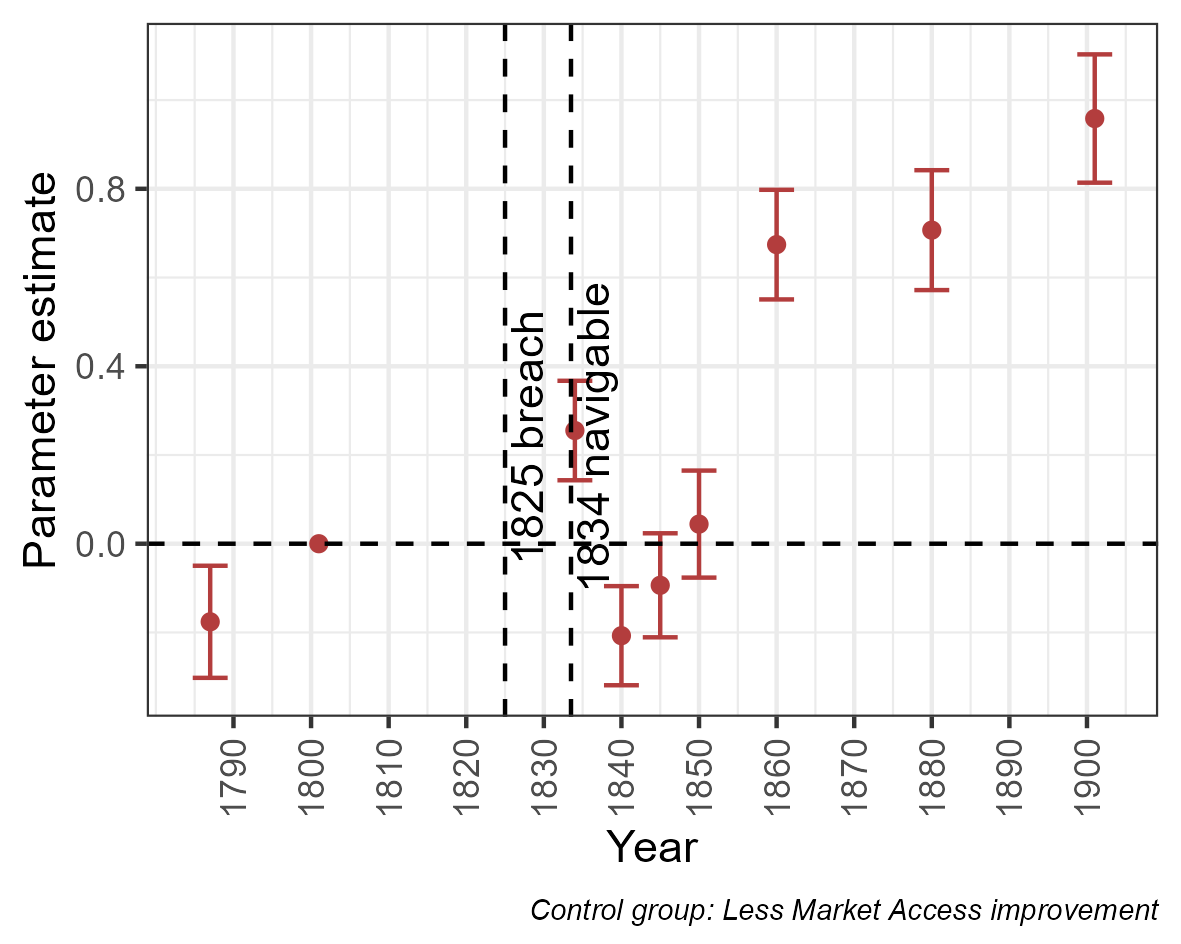
\includegraphics[width=\textwidth]{Plots/Mechanism/fertility_MA.png}
    \end{subfigure}
    \hfill
    \begin{subfigure}[b]{0.45\textwidth}
        \centering
        \caption{Fertility (dummy approach)} \label{fig:fert_dummy}
        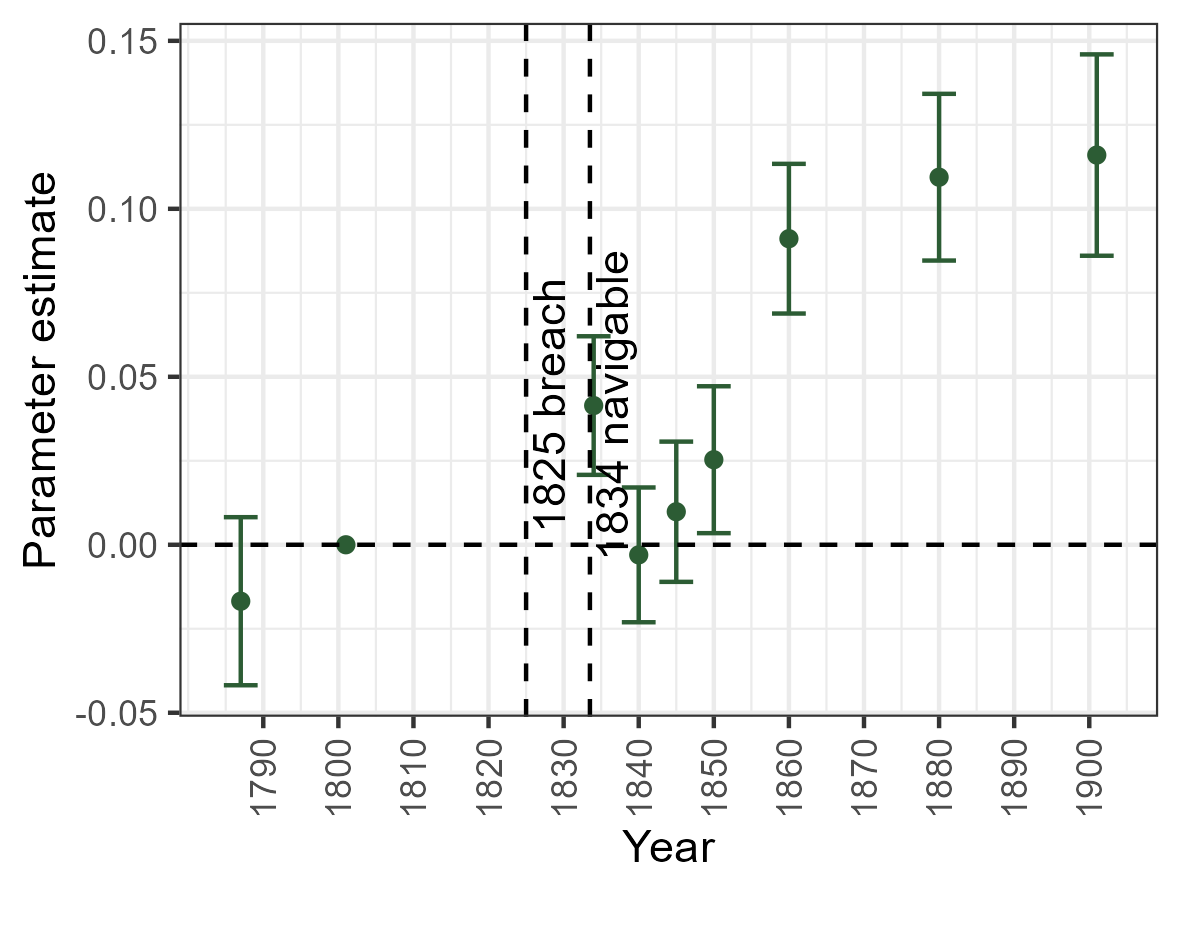
\includegraphics[width=\textwidth]{Plots/Mechanism/fertility_Dummy.png}
    \end{subfigure}
    \vspace{0.45cm}
    \begin{subfigure}[b]{0.45\textwidth}
        \centering
        \caption{Internal migration (MA approach)} \label{fig:migr_ma}
        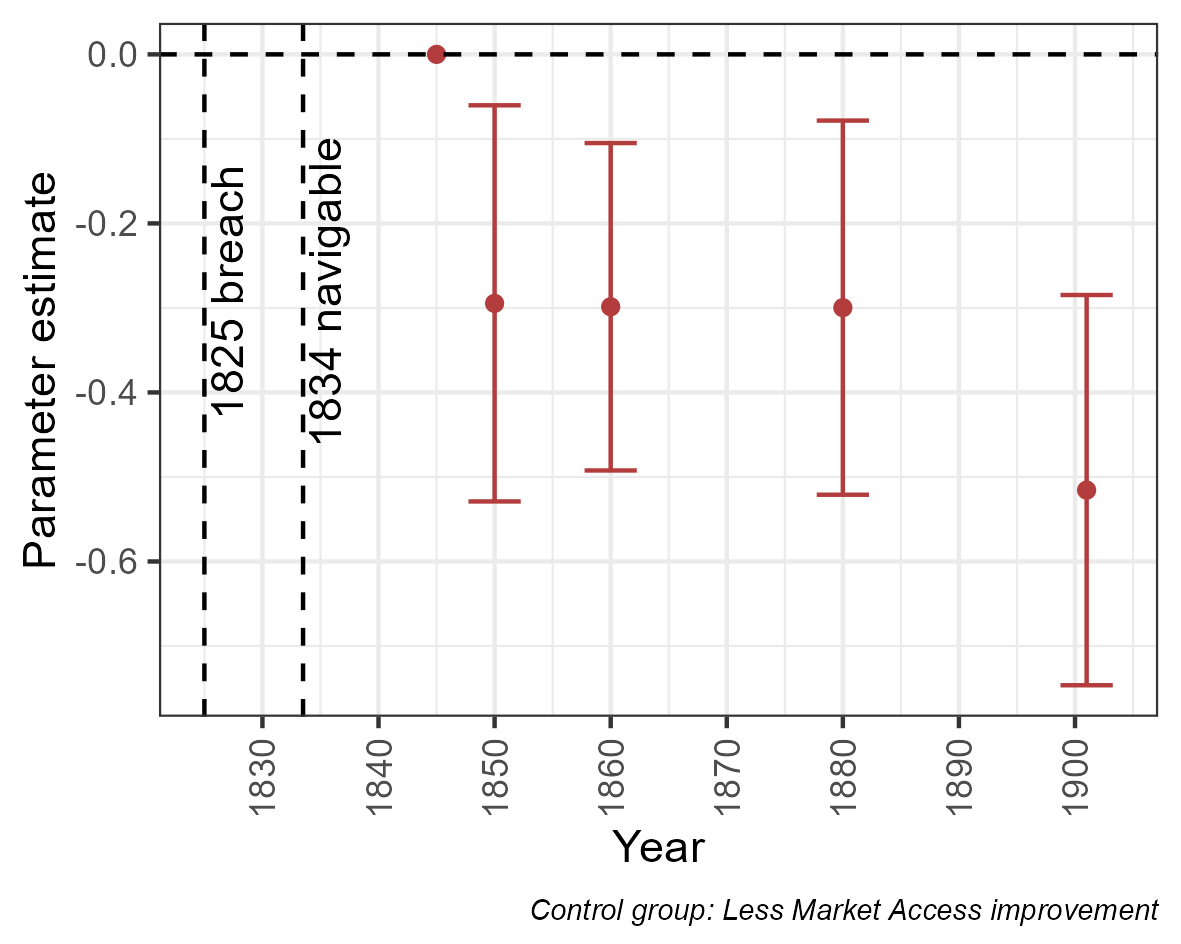
\includegraphics[width=\textwidth]{Plots/Mechanism/born_different_share_MA.png}
    \end{subfigure}
    \hfill
    \begin{subfigure}[b]{0.45\textwidth}
        \centering
        \caption{Internal migration (dummy approach)} \label{fig:migr_dummy}
        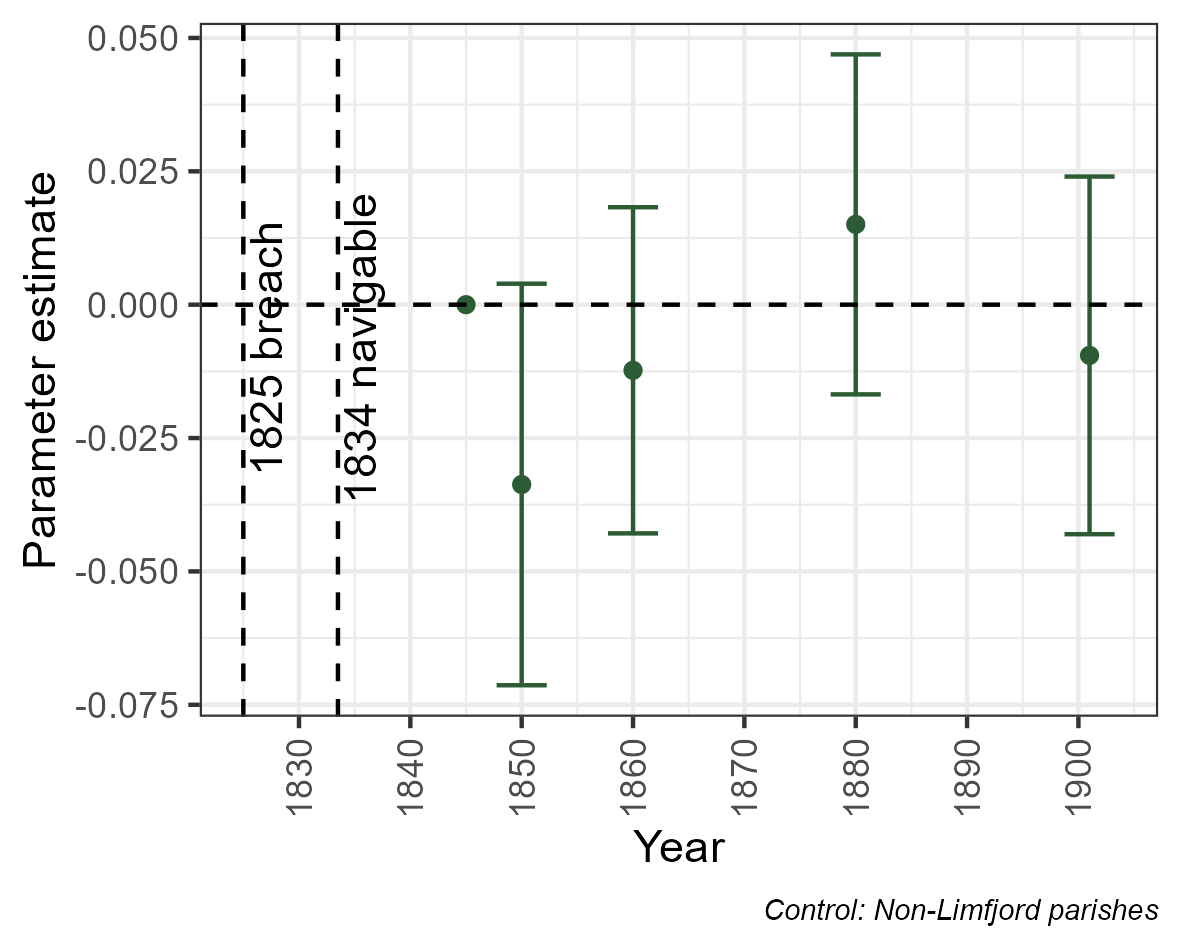
\includegraphics[width=\textwidth]{Plots/Mechanism/born_different_share_Dummy.png}
    \end{subfigure}
    \parbox{0.9\textwidth}{
    \caption*{\footnotesize \textit{Notes:} This shows the effect of the 1825 breach on indicators of fertility and migration. Panel (a) and panel (b) show the effect on the child-women ratio. Panels (c) and (d) show the effect on the number of people born in a different county, than where they usually live as a share of the total population in that parish. The results of panels (a) and (b) indicate that the channel caused fertility to increase. The results of panels (c) and (d) indicate, that migration either contributed negatively to the increase in population or did not contribute at all.  \\ \textit{Source: Danish census data}}
}
    \label{fig:migr_fert}
\end{figure}

\FloatBarrier

\section{The reverse natural experiment and external validity}

\subsection{Method and data}
If a causal effect has been identified, one implication is that it should be replicable across heterogeneous environments \citep{Peters2016}. This is the formal causal reasoning behind the classical arguments for replication studies and concerns of external validity. But it also gives a clue to a way of approaching it. What is truly sought after, when external validity is pursued, is a repetition of the same event in a completely different environment. If the effect is the same, this is evidence, that the effect is not just some quirk of the particular setup. The setting of this particular paper allows me to test exactly this. 

The Limfjord region was endowed with favorable first-nature geography after 1834. But this was not the first time the region had been lucky in the geomorphological lottery. The region was endowed with a similar channel in a similar location before the 1100s (see section 3 Historical background). But sometime between 1085 and 1208, the channel closed. In other words, the same natural experiment occurred. Only this time in reverse. Denmark in the 1100s had recently converted from paganism to Christianity, was dominated by Viking traditions and technology and did not have the benefit of modern science or enlightenment \citep{Roesdahl2022, milkandbutter}. Denmark of the 1100s is different from Denmark of 1834 in terms of all the important factors that otherwise impact economic performance in the long run. It is almost like comparing two entirely separate countries. But instead of comparing two countries separated in space, they are separated in time by 700 years. This also implicitly keeps the geography constant with the channel-availability as the obvious exception. That is, the only geography that varies in these two cases, is the exact same (mirror image) shock to first-nature geography. 

A key problem in this is that the amount of available data of the 1100s is very sparse to say the least. One available approach is the use of archaeological evidence as an indication of economic activity or population density. The idea comes out of the positive archaeological tradition of Settlement Scaling Theory, which simply utilizes that a larger settlement will generate more things to be discovered by archaeologists \citep{Ortman2020}. This approach has also seen application within economics \citep{Davis2002, Bakker2021Phonecians, Allen2023, Barjamovic2019}. A methodological innovation of the present paper is to derive and use Bayes' formula to calculate the implied timing and location of economic activity based on the dating and location of archaeological sites.

The Danish registry of archaeological sites 'Fund og fortidsminder' contains data on all archaeological sites reported by Danish museums and the national agency of culture and palaces. This data is publicly available.\footnote{All the data can be downloaded here: https://www.kulturarv.dk/fundogfortidsminder/Download/} The data contains a specific coordinate of the finding, a type (e.g. if it were coins, a former house, burial mount, etc.), and a range of years to which it is dated. The current version of the database contains 290.524 findings in total. But this includes all kinds of sites from the earliest palaeolithic until a few years before the present time. The focus is narrowed a bit on what likely contains useful information in this particular analysis. The data is limited to only include sites which are dated to somewhere between 750 and 1500 CE and only two types of findings: Coins and Buildings. Coins indicate that some amount of trade took place in and around this particular site. Buildings directly reflect population density. More people require more buildings, which increases the probability that remains will be left for archaeologists to discover. The database contains 3411 coin findings and 4396 findings of buildings. These observations are used to construct parish-level panels of economic activity.

An example is pertinent at this point: The finding with id 338 is a finding of coins, which can be dated to somewhere between 1300 and 1535. The site of the finding is at the decimal coordinate (14.92617, 55.02614). This is within the historic parish of Pedersker on the island of Bornholm. This means that some activity that caused coins to be used happened around this location in this time frame. A simple approach would then be to mark Pedersker with a '1', indicating that coins were found here for the years 1300-1535. Applying this principle to all parishes would then allow for the construction of an entire panel of the likely location of economic activity. The descriptive results from this procedure is shown in Figure \ref{fig:arch_desc} (details about this in the following). However, this measure causes places with more uncertain dating to be more likely to have economic activity associated with it. This is simply because the coins in Pedersker would show up multiple times, whereas a coin associated with e.g. a single year would only show up once, even though the coin with a smaller range arguably contains more information about the time and location of economic activity. Moreover, this simple method would reflect the inverse of what is of interest and this would make interpretation difficult. 

It is useful to think about this in terms of the probabilities the data represents. What is observed is information on the probability of years being associated with a finding: $P(t|finding)$ (e.g. 1300 to 1535 given coin in Pedersker parish). However, what is of interest is the opposite - $P(finding|t)$ - the probability that e.g. 1350 or 1400 is the actual year for which a finding was generated. Moreover, the amount of findings is of little use. It is no surprise that archaeologists find more things in places, where they have already found something. One finding will generate more excavations. For this reason, the intensive margin is not of interest, only the extensive margin is. $P(\{findings\}|t)$ expresses the probability of \textit{any} finding being generated at a specific time. Notice $\{findings\}$ with the curly brackets added. The curly brackets indicate the event that one or more findings are associated with a particular parish. However, this adds further complication to the analytical expression. But it can be derived,\footnote{See more details in the Appendix E.1.} that the formula for this can be expressed as 

\begin{equation}
\begin{split}
\label{eq:arch1}
P_i(\{findings\}|t)&=\left[1-\prod_{c=1}^{K_i} \left( 1 - P(t|finding_c) \right)\right] P(\{findings\}) \\
\end{split}
\end{equation}

where, assuming $P(t|finding)$ is a uniform distribution,

\begin{equation}
\begin{split}
\label{eq:arch12}
P(t|finding_c)& = 1[t\in [Y_{min}^c;Y_{max}^c]] \left(\frac{1}{Y_{max}^c - Y_{min}^c}\right).
\end{split}
\end{equation}

Here $P_i(\{findings\}|t)$ is the probability of any findings (coins or buildings) having been generated at time $t$ for later discovery in parish $i$. This is calculated over all the archaeological findings in that parish $c \in [1, K_i]$ and the particular dating distribution of each finding (given by a range of years $Y_{min},\: Y_{max}$). All of the is multiplied by the prior probability that any findings would have been generated.\footnote{Whether archaeologists' dating ranges should be interpreted as a uniform distribution is not given. An obvious alternative is to assume a normal distribution, where the uncertainty represents a 95 percent confidence interval from the distribution. Results using this approach are shown in Appendix E.3. These results are qualitatively equivalent.} Estimating this probability for every year and for every parish generates a panel of economic activity across all parishes. 

This can be calculated by drawing random samples from this distribution. This is quite simply a matter of drawing a random year in the range of years, that a particular finding has been dated to. This is repeated 1000 times. Each time it is checked whether any particular year and parish pair has any finding associated with it in this random draw. These are all draws from the probability distribution of interest and with enough samples an adequate representation of it comes from simply counting the frequency with which draws are successful. 

This data enters the general approach presented in section 4. The outcome in this case is the probability that a coin finding was generated in a specific parish in a specific year (or $\pm 25$ within a specific year to be more exact).

\begin{equation}
\label{eq:eq7_4}
P_i(Coin|t) = \alpha_t + \alpha_i + \sum_{j = 750, j\neq 1000}^{1500} 1[t=j]\times Affected_{i}\beta_{j}  + \varepsilon_{it}
\end{equation}

As before, $Affected$ is measured both in terms of a dummy and the estimated change in market access. Inference is made with a clustered bootstrap, which resamples the panel from the 1000 samples drawn from the distribution of equation \ref{eq:arch1}. A further concern is that soil types might cause endogeneity. It might be that places with more fertile soil types had a differential developmental path \citep{HeavyPlough2016, WinnersAndLosers2022}. The western part of the Limfjord is rich in fertile soil. At the same time, the soil type might also influence the rate of survival of archaeological sites. 

To counter this, propensity score matching is used. The aim of this is to ensure that parishes affected by the channel closing are compared to parishes, which in terms of soil type, are similar parishes to those not affected. The propensity score is estimated using extreme gradient boosting trees \citep{chen2016xgboost}, which is a machine learning technique suitable for classification using tabular data, which can be thought of as a generalization of a random forest \citep{Breiman2001}. Data on soil types are obtained from \cite{Pedersen2019}. Only the soil types found in at least 10 percent of parishes are used, otherwise the model overfits by utilizing the fingerprint of allocation of more unique soil types. The procedure estimates a model, which predicts the probability (propensity), that a given parish is a west Limfjord parish based on the soil types in the parish

\begin{equation}
\label{eq:eq7_5}
P_i(Affected|\mathbf{X}_i) = f(\mathbf{X}_i)+\varepsilon_i.
\end{equation}

Each parish in the west Limfjord, is then matched with a counterpart, which has the most similar propensity score outside the Limfjord region. This represents the match with the most similar soil type. This is done in a greedy fashion - without replacement - ensuring that each parish is matched with \textit{one} other parish which at the same time is not the match of any other affected parish. Figure \ref{fig:prop_score} shows the propensity score of parishes included in the sample before and after matching. Notice that after matching, the distributions of propensity scores are almost identical across the west Limfjord and the reference group. 

\begin{figure}
    \centering
    \caption{Soil type propensity scores}
    \begin{subfigure}[b]{0.45\textwidth}
        \centering
        \caption{Propensity score before matching} \label{fig:prop1}
        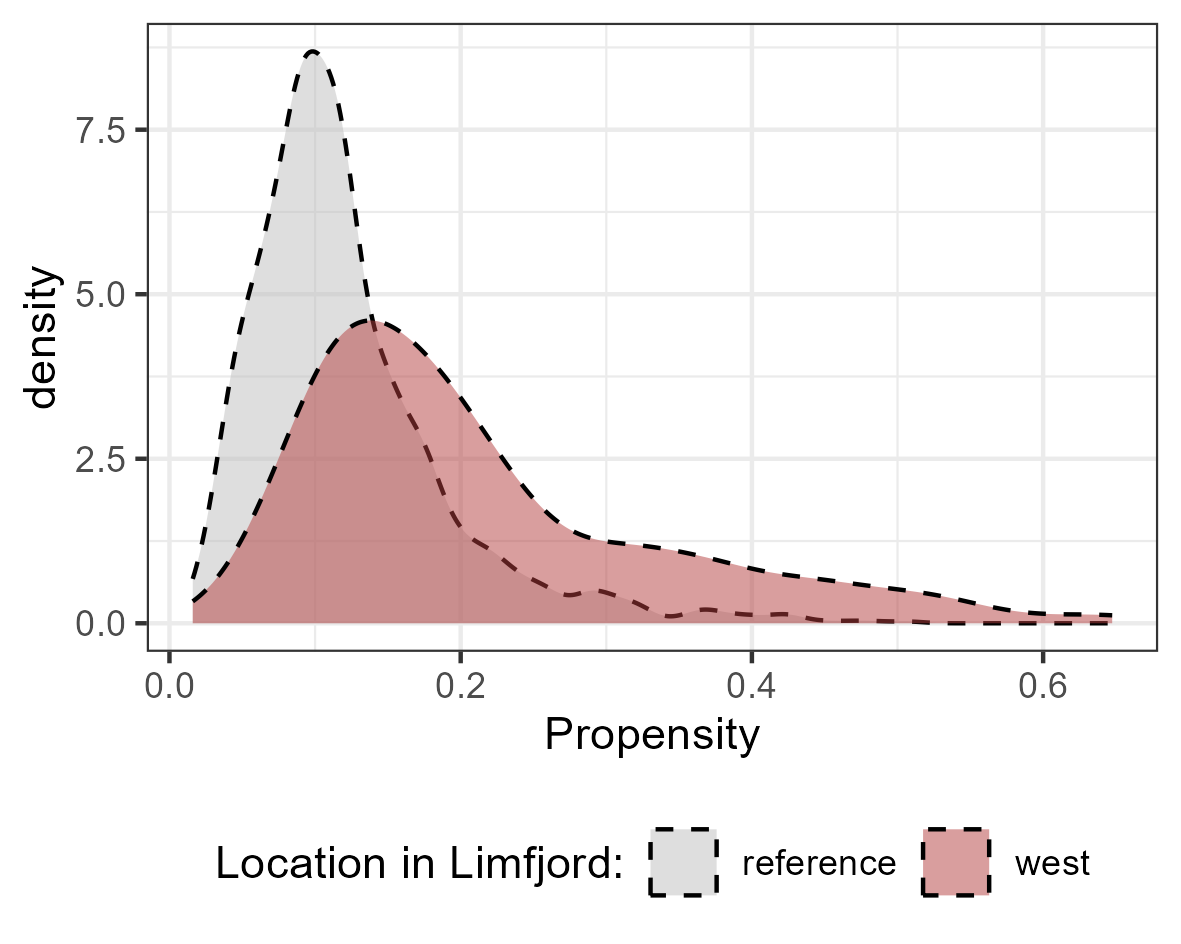
\includegraphics[width=\textwidth]{Plots/Propensity_before.png}
    \end{subfigure}
    \hfill
    \begin{subfigure}[b]{0.45\textwidth}
        \centering
        \caption{Propensity score after matching} \label{fig:prop2}
        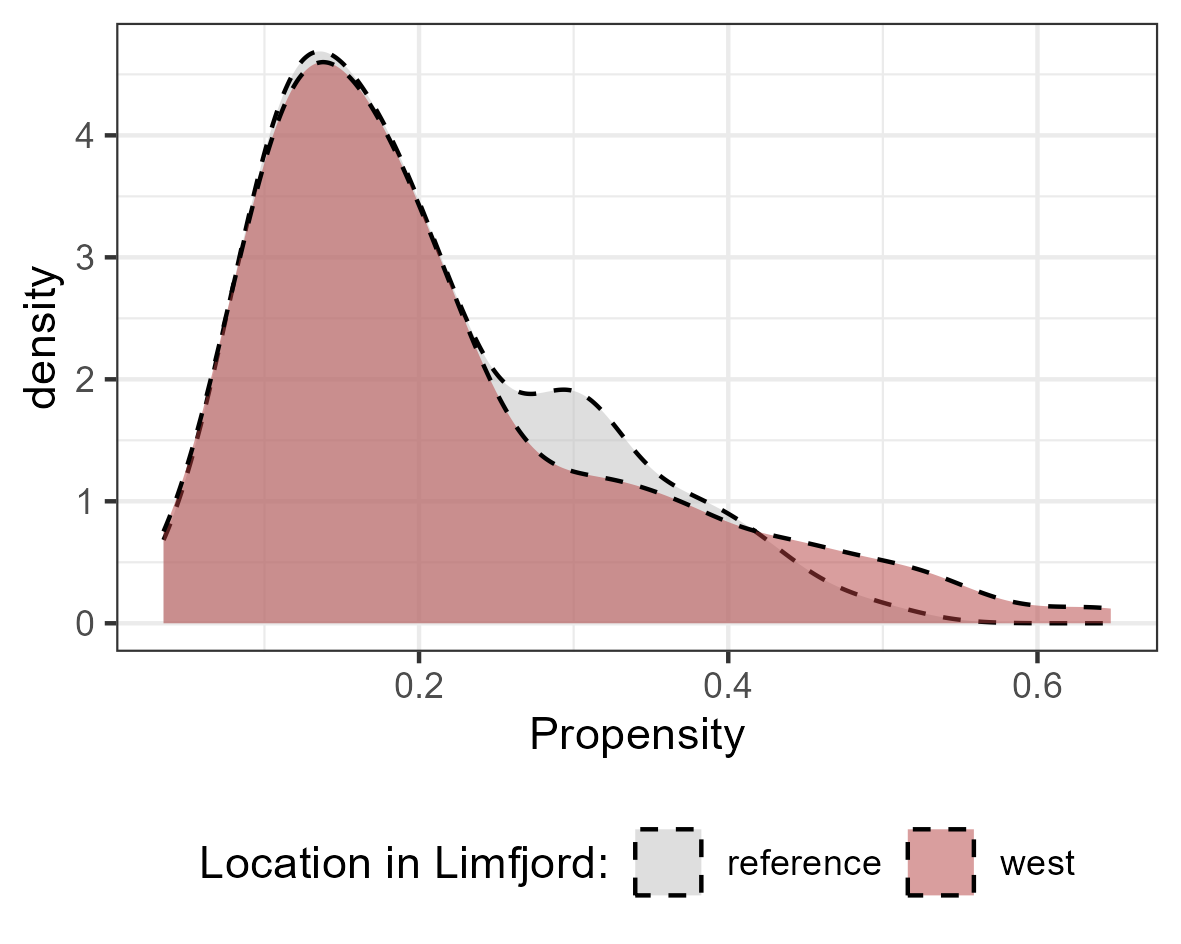
\includegraphics[width=\textwidth]{Plots/Propensity_after.png}
    \end{subfigure}
    \parbox{0.9\textwidth}{
    \caption*{\footnotesize \textit{Notes:} Propensity score between the west Limfjord and the reference group before and after matching. Propensity scores are estimated using extreme gradient boost. Matching is done with a greedy matching procedure in random order.}
}
    \label{fig:prop_score}
\end{figure}

Before showing anything using the estimated probabilities, Figure \ref{fig:arch_desc} simply displays the mean number of coin findings in various regions of the Limfjord as well as in the remainder of the country, spanning from 750 to 1500. This is suggestive of the effect of the closing of a channel between 1085 and 1208 and its impact on the west Limfjord region. The plot demonstrates a gradual rise in coin findings, especially in the east Limfjord and the rest of the country, following the channel closure, whereas the west and middle Limfjord regions remain at lower levels. This finding suggests that the west and middle Limfjord regions may have experienced an economic and commercial decline during this period. This reveals that an effect can be observed even with a straightforward approach. However, more uncertain observations have more weight in this very simple descriptive plot. Regression results, that accounts for this, are presented in Figure \ref{fig:arch_reg} and \ref{fig:arch_reg_boot} and table \ref{tab:arch1}.

\begin{figure}
     \centering
     \caption{Simple count of coin findings}\label{fig:arch_desc}
     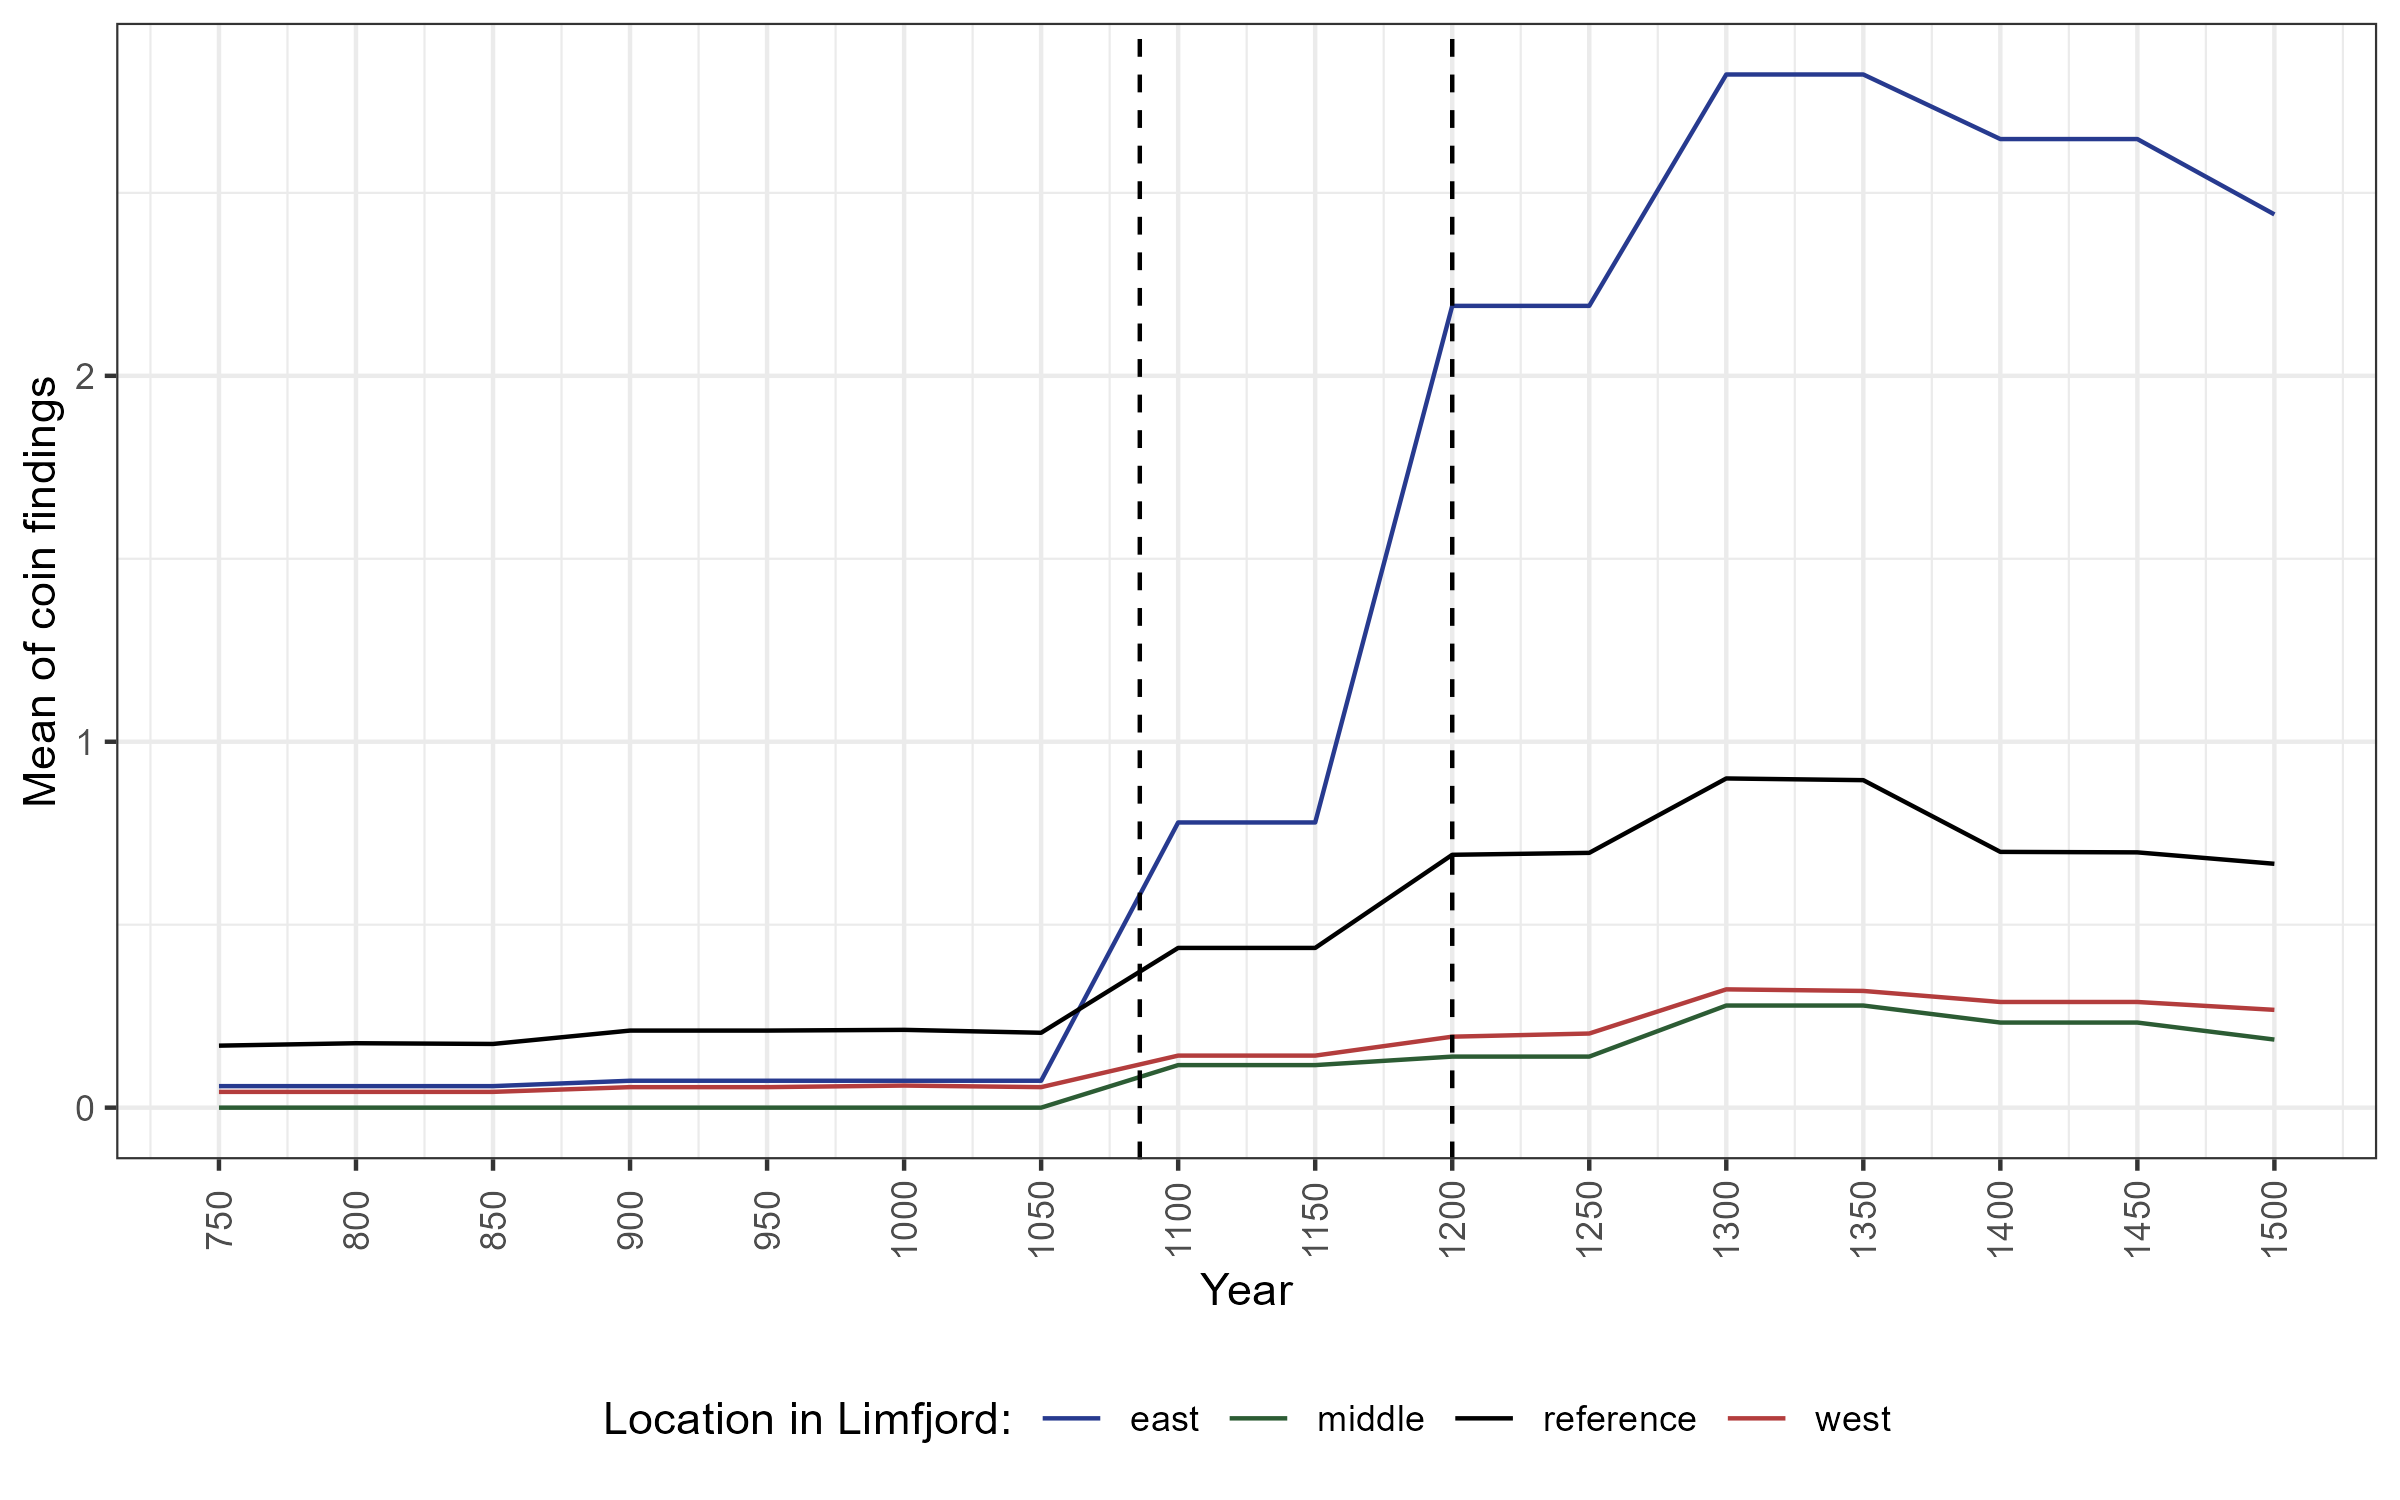
\includegraphics[width=\textwidth]{Plots/Arch_descriptive.png}
     \parbox{0.9\textwidth}{
     \caption*{\footnotesize \textit{Notes:} This plot shows the average number of coin findings, where coin findings are simply counted if they are potentially attributable to a particular year. This is done for the West, Middle and East Limfjord region as well as for the rest of the country as reference. \\ \textit{Source: Danish registry of archaeological findings}}
}
     \label{fig:regpops}
\end{figure}

\FloatBarrier
\subsection{Results}

Figure \ref{fig:arch_reg} and table \ref{tab:arch1} provide more reliable estimations of the probability of archaeological findings being generated in the affected regions of the Limfjord. Figure \ref{fig:arch_reg_boot} shows the parameter distribution in 1350 yielded by the sampling procedure presented. The regression table presents the results of archaeological regressions for the full sample of all Denmark and a matched sample, using both the dummy definition of being affected and the change in market access approach. The outcome is the probability that a coin finding or building was generated in the area covered by that parish within $\pm 25$ years of the reported year. 

The parameters from the Market Access approach should be interpreted as semi-elasticities, i.e. how does the probability of a coin being generated change with a relative change in market access? These are approximately interpretable as percentage changes. I.e. a 1 percent decrease in Market Access led to a 13-19 percent change in the probability of a coin finding being generated in 1350 - 150 years after the channel closed (columns 1 and 5). Equivalently, it led to a reduction in the chance of buildings being generated as archaeological findings by 6 to 8 percent (columns 3 and 7). The parameters for the dummy approach can be interpreted as the change in the probability that findings were generated from a West Limfjord parish compared to other parishes. In 1350, the chance of coin findings being generated had fallen by around 1.5 or 1.9 percent  (columns 2 and 6), and the probability of buildings to become archaeological findings had decreased by 0.6 to 1 percent (columns 4 and 8). 

For all these estimates it is seen, that there is a rather stable effect size before 1085-1208 of approximately zero, but after this the probability sharply declines. Appendix E.2. provides tables of all parameters. It is worth considering whether these results can be spurious because of the added layer of uncertainty added by the Monte Carlo method. But the standard errors used take this added uncertainty into account. Figure \ref{fig:arch_reg_boot} shows parameter distribution in 1350 given by the bootstrap samples.

Whichever methodological alternatives are employed, the results show a large negative effect of the closure of the channel for the affected parishes. The results suggest that the closure of the channel between 1085 and 1208 had a significant impact on the west Limfjord regions, causing a decline in the probability of coin findings and buildings being generated in those areas. These findings are consistent with the hypothesis that the channel closure caused economic and commercial decline in the region. It is not possible to do an apples-to-apples comparison to the census data for the Agger channel of 1834. But it is certainly noteworthy that the parameters are of similar sign and magnitudes for these two channels in the same location. This corroborates the external validity of the main result: First-nature geography is the cause of the location of prosperity across very different societies. 

\begin{figure}
    \centering
    \caption{Archaelogical results}
    \begin{subfigure}[b]{0.45\textwidth}
        \centering
        \caption{Coins: Market access approach} \label{fig:arch1a}
        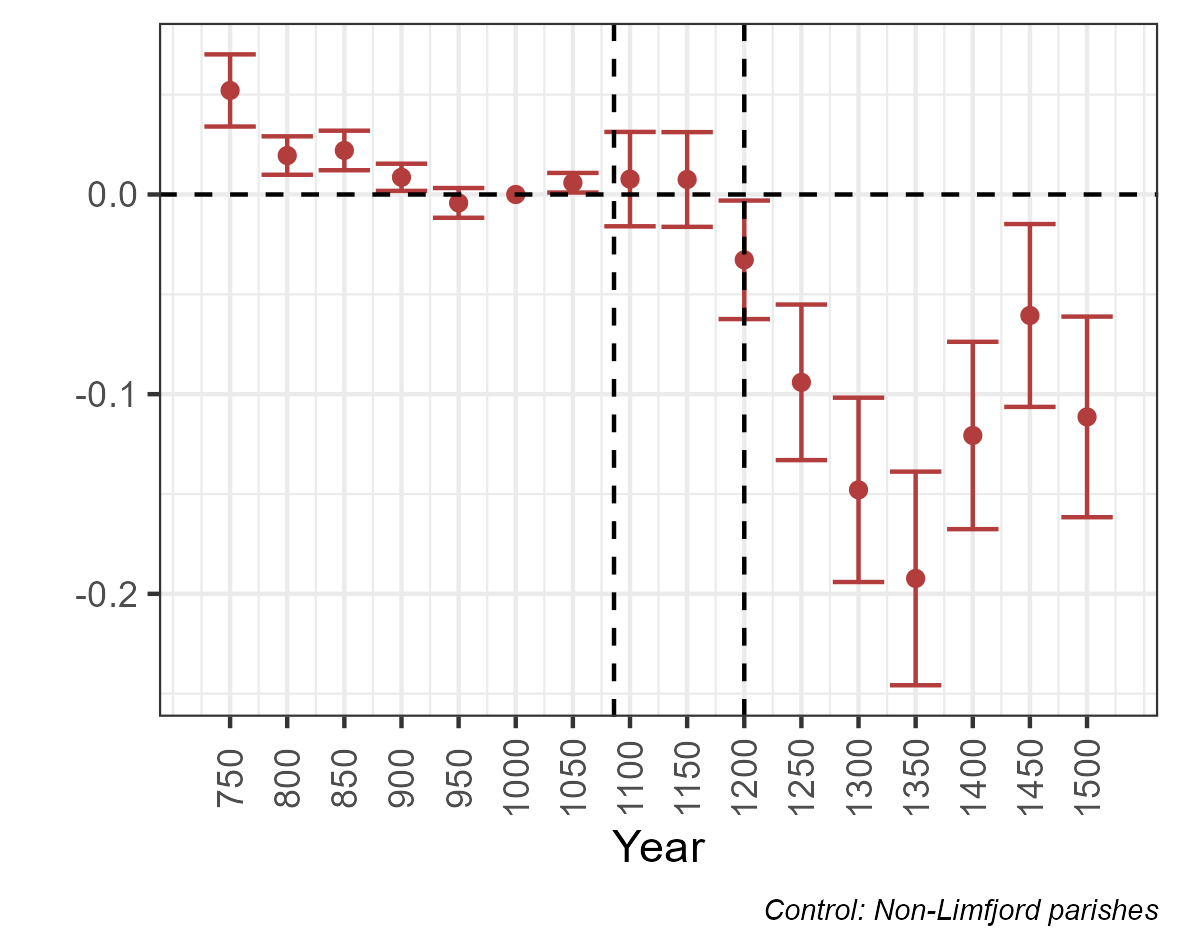
\includegraphics[width=\textwidth]{Plots/Regression_plots/arch_MA_coins.png}
    \end{subfigure}
    \hfill
    \begin{subfigure}[b]{0.45\textwidth}
        \centering
        \caption{Coins: Dummy approach} \label{fig:arch1b}
        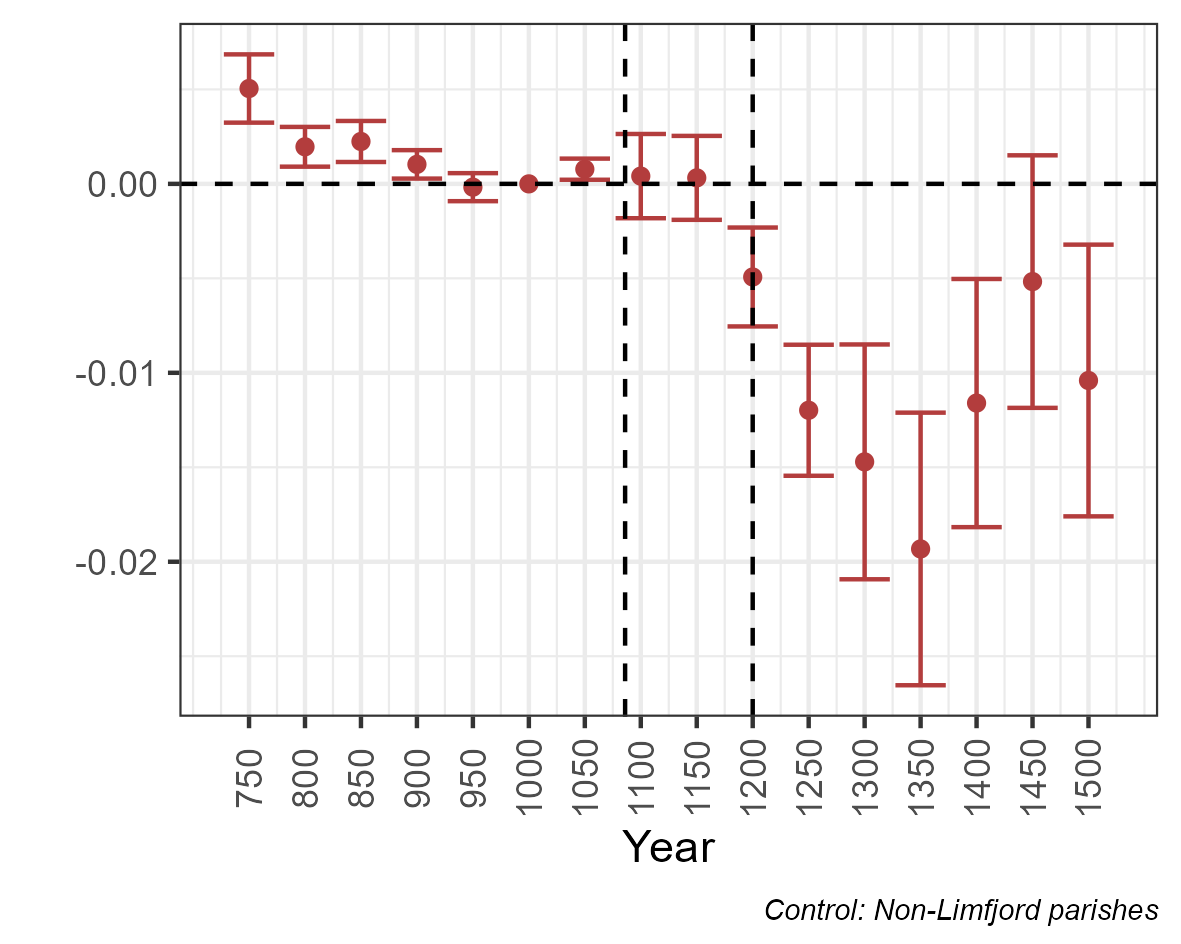
\includegraphics[width=\textwidth]{Plots/Regression_plots/arch_dummy_coins.png}
    \end{subfigure}
    \vspace{0.45cm}
    \begin{subfigure}[b]{0.45\textwidth}
        \centering
        \caption{Buildings: Market access approach} \label{fig:arch1c}
        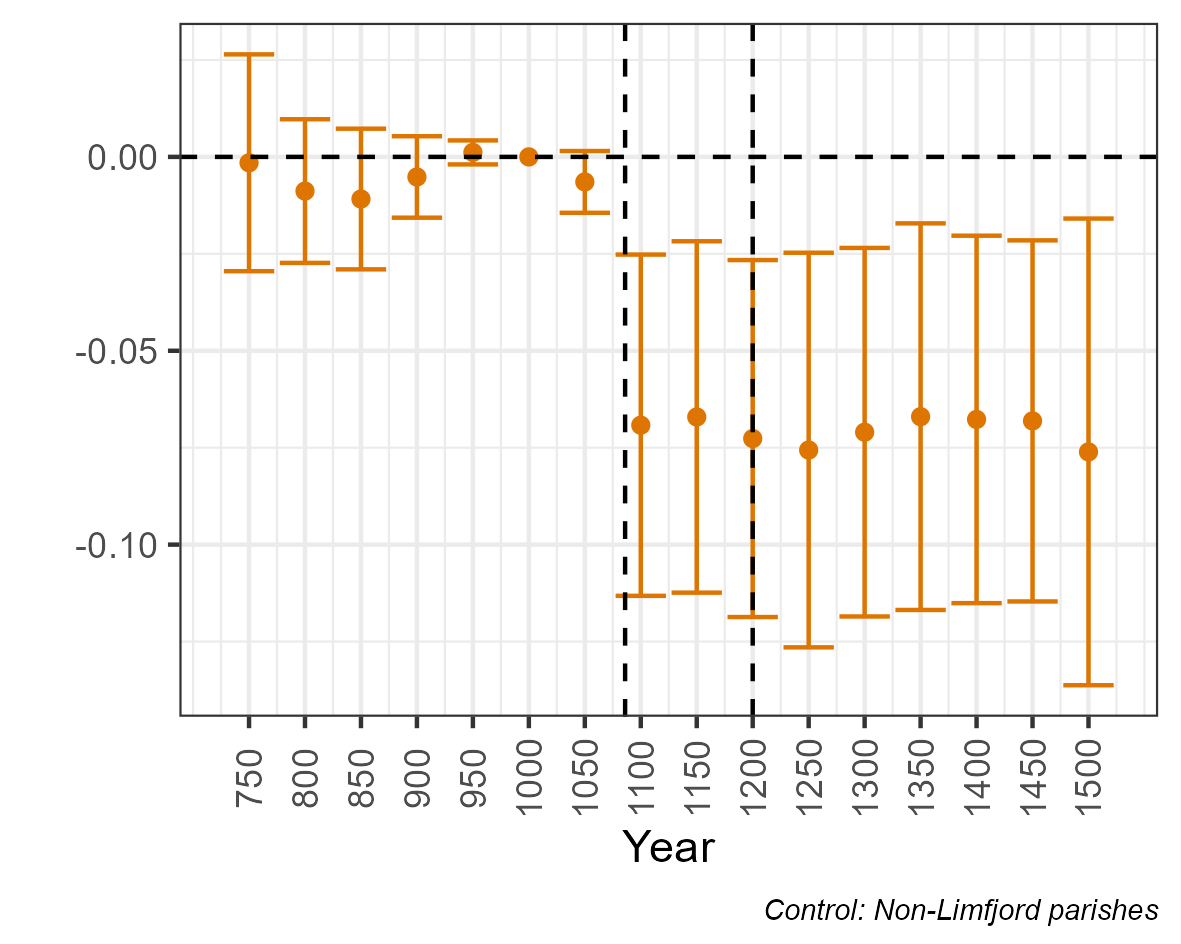
\includegraphics[width=\textwidth]{Plots/Regression_plots/arch_MA_buildings.png}
    \end{subfigure}
    \hfill
    \begin{subfigure}[b]{0.45\textwidth}
        \centering
        \caption{Buildings: Dummy approach} \label{fig:arch1d}
        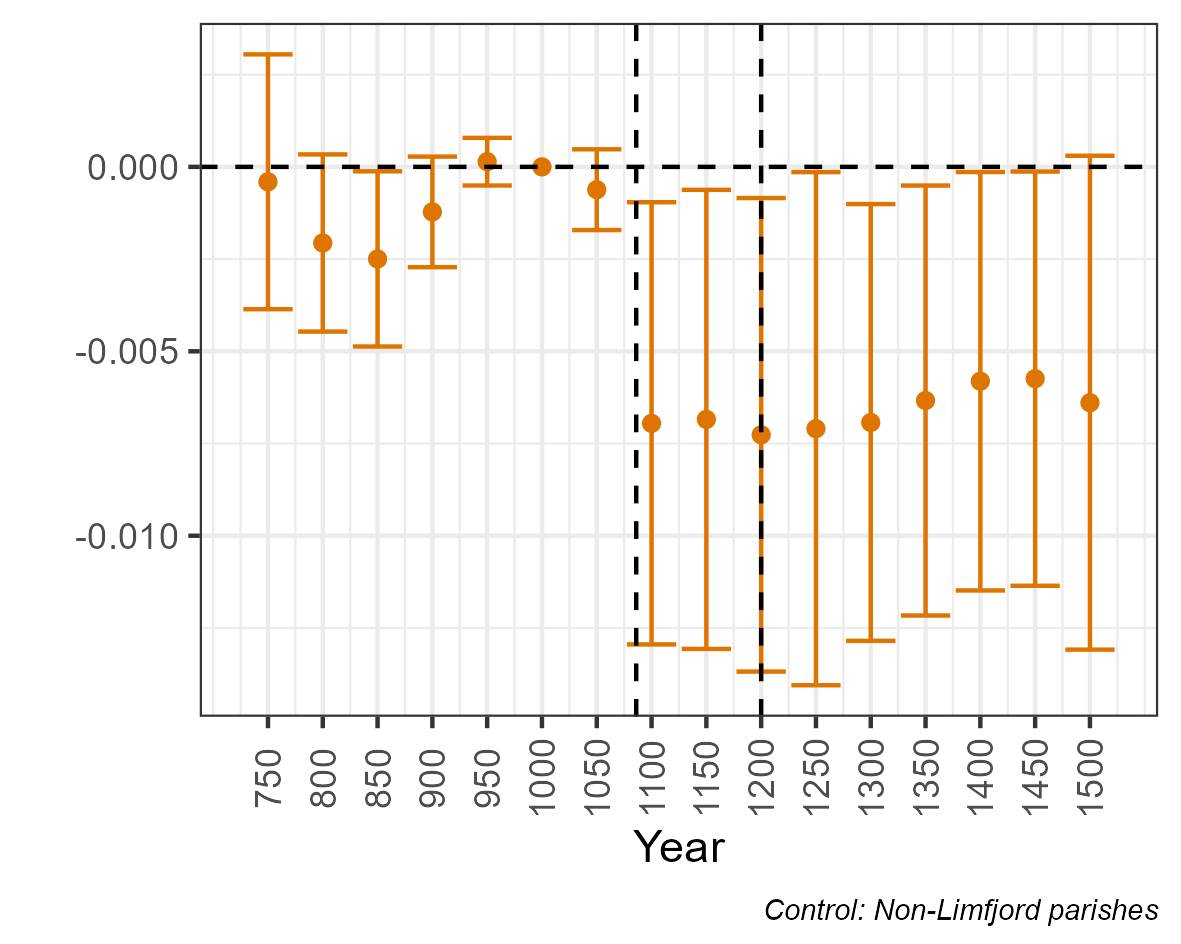
\includegraphics[width=\textwidth]{Plots/Regression_plots/arch_dummy_buildings.png}
    \end{subfigure}
    \parbox{0.9\textwidth}{
    \caption*{\footnotesize \textit{Notes:} Effect of the closing of the channel on the probability of archaeological findings. Error bars represent 95 percent confidence intervals based on clustered bootstrap errors. Panel (a) shows results for coin findings relying on the market access approach. Panel (b) also shows results for coins but using the dummy approach. Panel (c) shows results for buildings using the market access approach. Panel (d) shows the results for buildings using the dummy approach.  \\ \textit{Source: Danish registry of archaeological findings}}
}    \label{fig:arch_reg}
\end{figure}


\begin{figure}
    \centering
    \caption{Distribution of parameter estimates in 1350}
    \begin{subfigure}[b]{0.45\textwidth}
        \centering
        \caption{Coins: Market access approach} \label{fig:distri_a}
        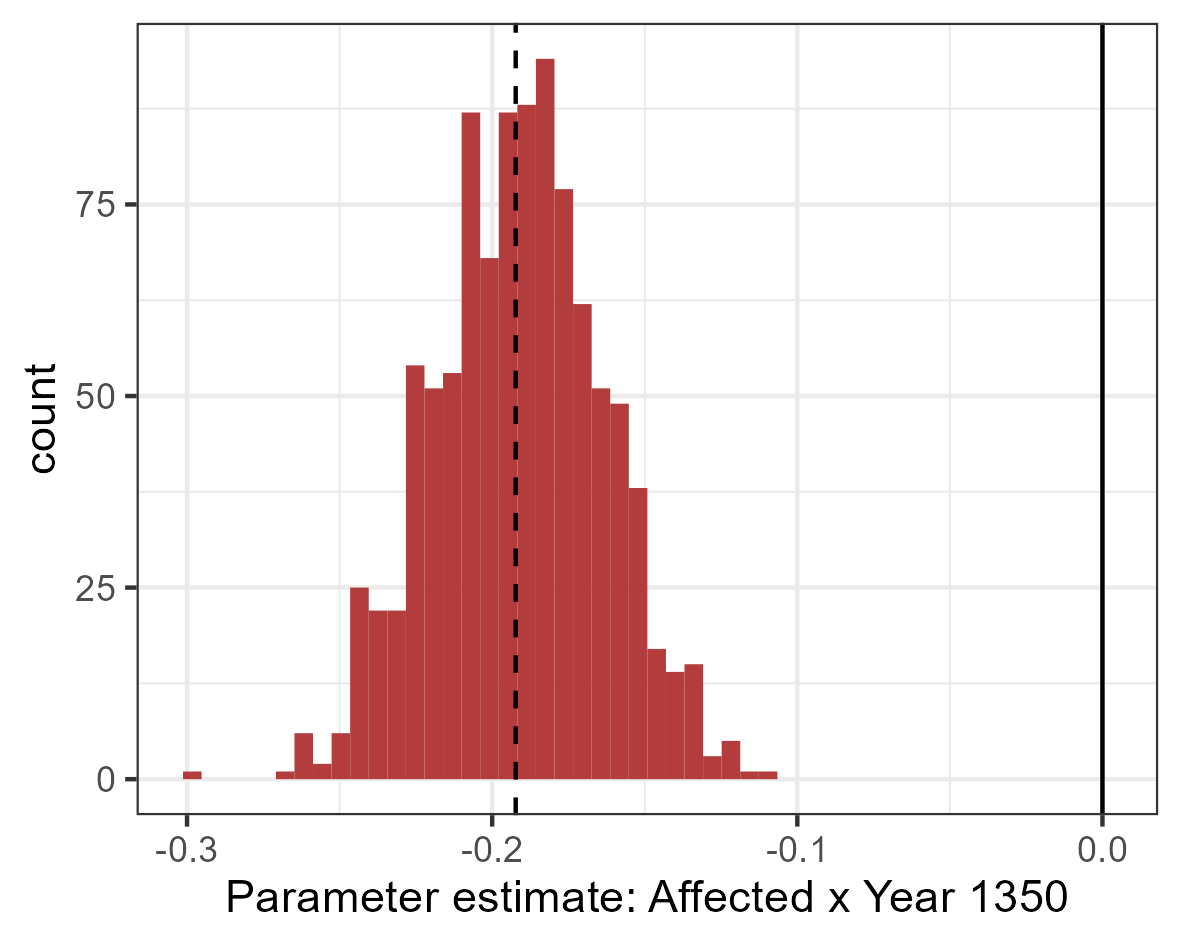
\includegraphics[width=\textwidth]{Plots/Regression_plots/arch_MA_coins_boot.png}
    \end{subfigure}
    \hfill
    \begin{subfigure}[b]{0.45\textwidth}
        \centering
        \caption{Coins: Dummy approach} \label{fig:distri_b}
        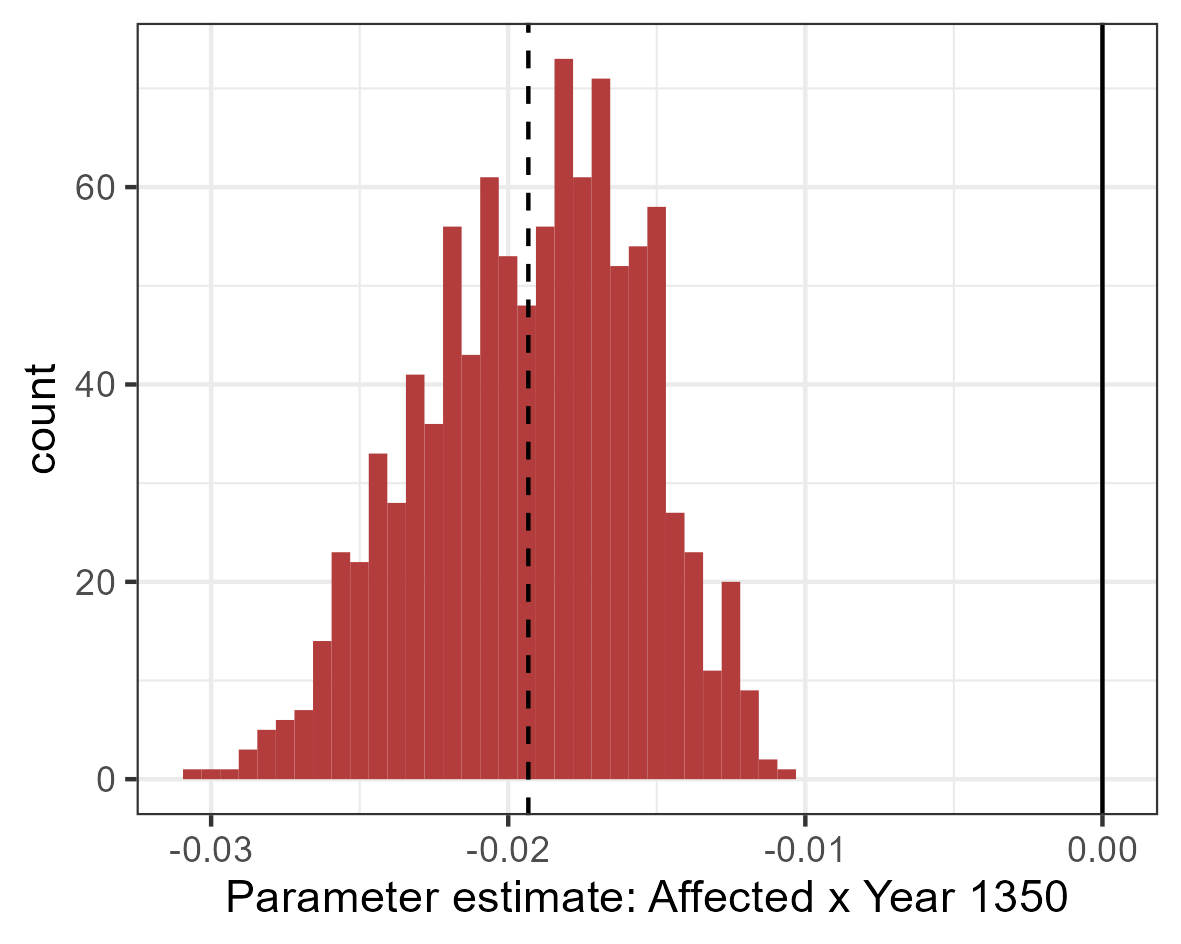
\includegraphics[width=\textwidth]{Plots/Regression_plots/arch_dummy_coins_boot.png}
    \end{subfigure}
    \vspace{0.45cm}
    \begin{subfigure}[b]{0.45\textwidth}
        \centering
        \caption{Buildings: Market access approach} \label{fig:distri_c}
        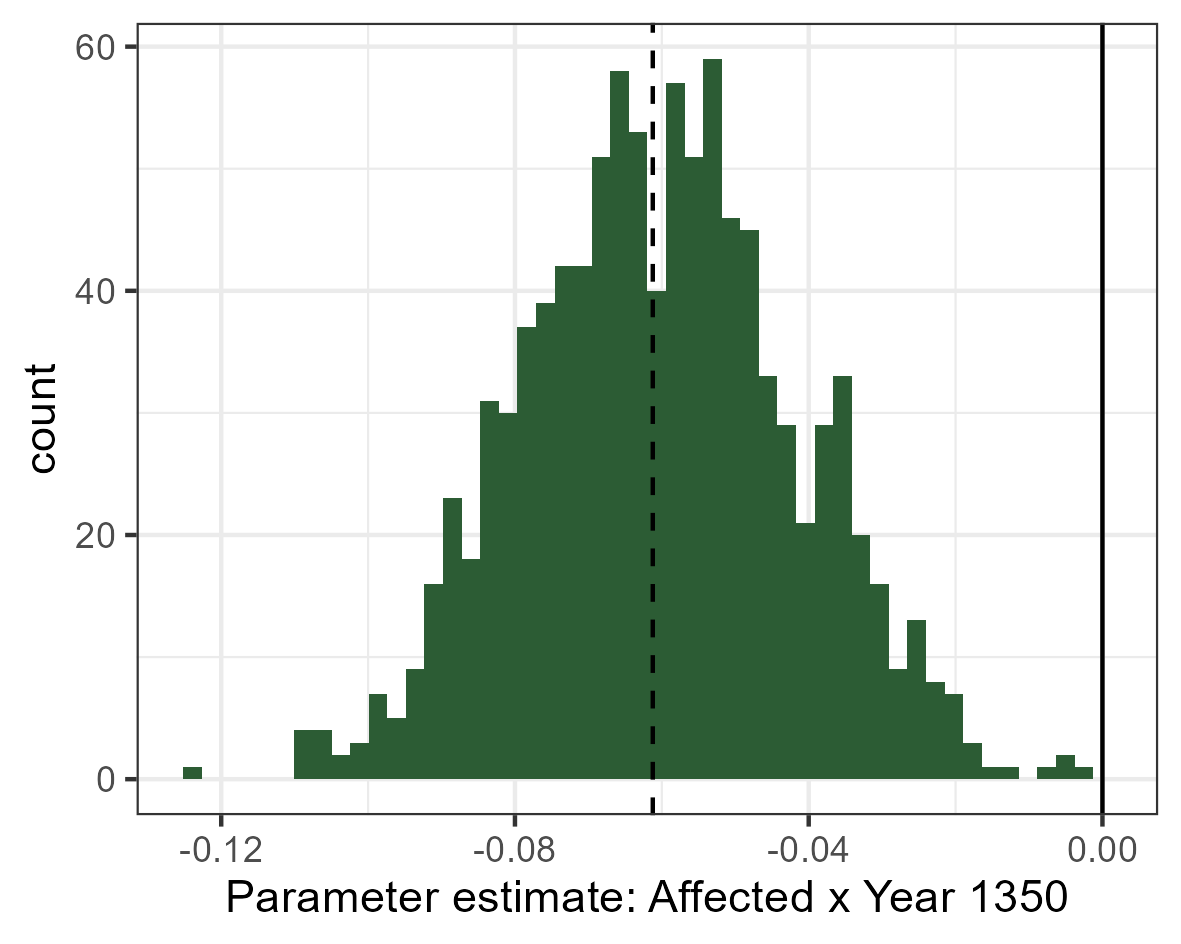
\includegraphics[width=\textwidth]{Plots/Regression_plots/arch_MA_buildings_boot.png}
    \end{subfigure}
    \hfill
    \begin{subfigure}[b]{0.45\textwidth}
        \centering
        \caption{Buildings: Dummy approach} \label{fig:distri_d}
        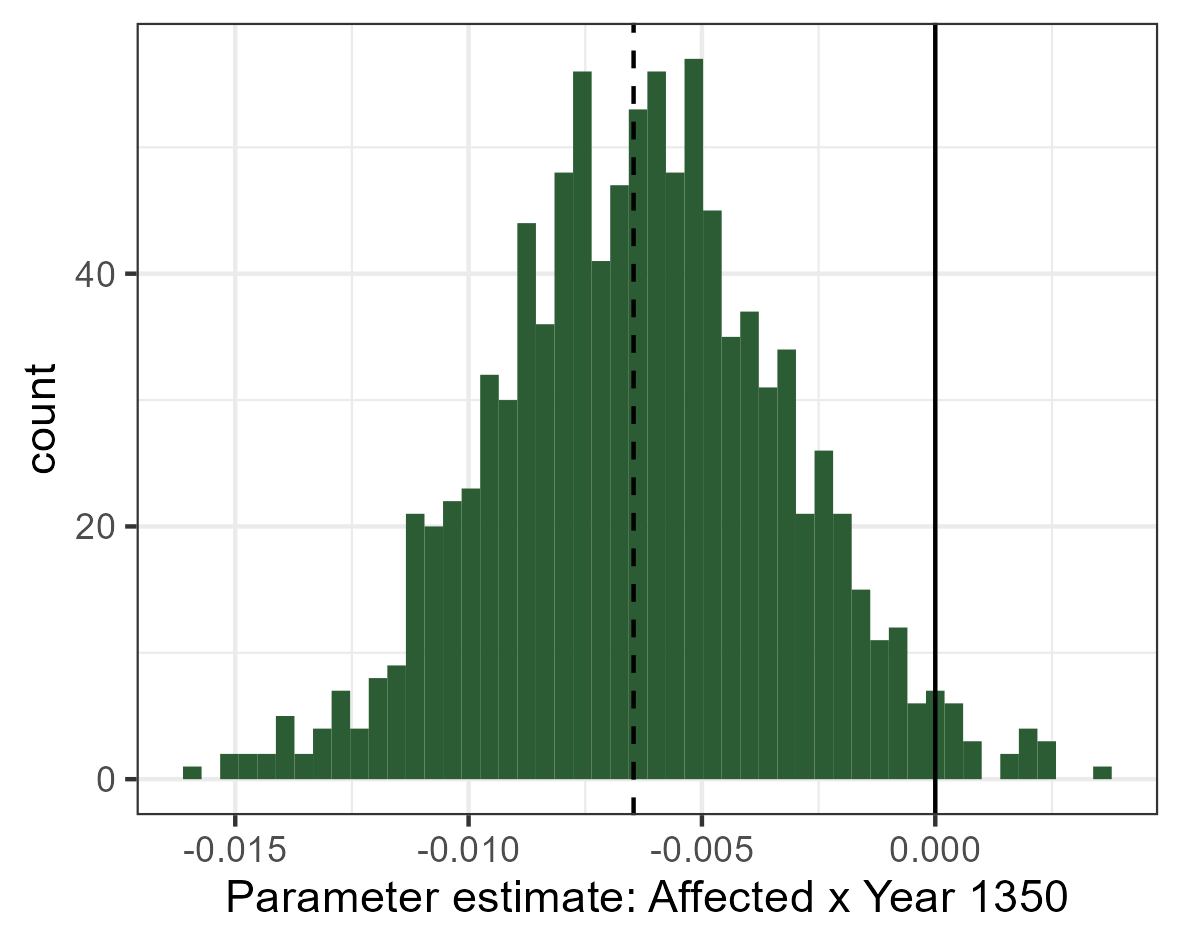
\includegraphics[width=\textwidth]{Plots/Regression_plots/arch_dummy_buildings_boot.png}
    \end{subfigure}
    \parbox{0.9\textwidth}{
    \caption*{\footnotesize \textit{Notes:} This shows 1000 draws from the bootstrap procedure, which takes classical (clustered) statistical uncertainty as well as dating uncertainty into account. Panel (a) shows the distribution of the effect on coin using the market access approach. Panel (b) shows the effect on coins using the dummy approach. Panel (c) shows the effect on buildings using the market access appraoch. Finally panel (d) shows the effect on buildings using the dummy approach. The dotted line is the parameter shown in table \ref{tab:arch1}. \\ \textit{Source: Danish registry of archaeological findings}}
}
    \label{fig:arch_reg_boot}
\end{figure}

\begin{landscape}
\begin{table}
\centering
\caption{Archaeological regression results} \label{tab:arch1}
\footnotesize
\begin{tabular}{lcccccccc}
   \tabularnewline \midrule \midrule
                                                    & \multicolumn{4}{c}{Full sample}                                                    & \multicolumn{4}{c}{Matched sample} \\
   \midrule
   Outcome:                                         & \multicolumn{2}{c}{Coin findings} & \multicolumn{2}{c}{Buildings}                  & \multicolumn{2}{c}{Coin findings}               & \multicolumn{2}{c}{Buildings}\\
                                                    & (1)             & (2)             & (3)                   & (4)                    & (5)                    & (6)                    & (7)            & (8)\\  
                                                    & MA              & Dummy           & MA                    & Dummy                  & MA                     & Dummy                  & MA             & Dummy \\ 
   \midrule
   Year950 $\times$ Affected                        & -0.0042         & -0.0002         & 0.0011                & 0.0002                 & -0.0177$^{*}$          & -0.0021$^{*}$          & 0.0008          & $-8.62\times 10^{-6}$\\    
                                                    & (0.0038)        & (0.0004)        & (0.0018)              & (0.0003)               & (0.0096)               & (0.0011)               & (0.0039)        & (0.0006)\\   
   Year1050 $\times$ Affected                       & 0.0059$^{**}$   & 0.0008$^{***}$  & -0.0063$^{**}$        & -0.0007                & 0.0051                 & 0.0006                 & -0.0083         & -0.0012\\   
                                                    & (0.0025)        & (0.0003)        & (0.0032)              & (0.0006)               & (0.0039)               & (0.0005)               & (0.0064)        & (0.0010)\\   
   Year1150 $\times$ Affected                       & 0.0075          & 0.0003          & -0.0681$^{***}$       & -0.0065$^{*}$          & 0.0320                 & 0.0036                 & -0.0705$^{**}$  & -0.0078\\   
                                                    & (0.0121)        & (0.0011)        & (0.0170)              & (0.0033)               & (0.0245)               & (0.0029)               & (0.0318)        & (0.0051)\\   
   Year1250 $\times$ Affected                       & -0.0941$^{***}$ & -0.0120$^{***}$ & -0.0772$^{***}$       & -0.0066$^{*}$          & -0.1216$^{***}$        & -0.0150$^{***}$        & -0.0829$^{***}$ & -0.0093$^{*}$\\   
                                                    & (0.0199)        & (0.0018)        & (0.0193)              & (0.0038)               & (0.0350)               & (0.0045)               & (0.0318)        & (0.0054)\\   
   Year1350 $\times$ Affected                       & -0.1923$^{***}$ & -0.0193$^{***}$ & -0.0612$^{***}$       & -0.0065$^{**}$         & -0.1408$^{***}$        & -0.0159$^{***}$        & -0.0669$^{**}$  & -0.0076\\   
                                                    & (0.0273)        & (0.0037)        & (0.0185)              & (0.0031)               & (0.0414)               & (0.0058)               & (0.0297)        & (0.0046)\\   
   \midrule
   Observations                                     & 29,568          & 29,568          & 29,568                & 29,568                 & 7,424                  & 7,424                  & 7,424          & 7,424\\  
   Parishes                                         & 1848            & 1848            & 1848                  & 1848                   & 464                    & 464                    & 464            & 464\\
   \midrule 
   Parish FE                                        & Yes             & Yes             & Yes                   & Yes                    & Yes                    & Yes                    & Yes            & Yes\\  
   Year FE                                          & Yes             & Yes             & Yes                   & Yes                    & Yes                    & Yes                    & Yes            & Yes\\
   \midrule \midrule
\end{tabular}
\parbox{1\textwidth}{
\caption*{\footnotesize \textit{Notes:} Archaeological regression results. Clustered bootstrap errors in parenthesis. Clustered at the parish level and sampled from the Monte Carlo procedure samples. Columns 1-4 show results using the full sample of all Denmark. Columns 5-8 show results for a matched sample. All the even columns show results using the dummy definition of being affected. All the uneven columns show results using the change in market access approach. The outcome is the probability that a given finding type was generated in the area covered by that parish within $\pm$25 years of the reported year. A parameter estimate for all years 750, 800, ..., 1500 can be found in the Appendix E.2. *** $p< 0.01$ ** $p< 0.05$ * $p< 0.10$. \\ \textit{Source: Danish registry of archaeological findings}}
}
\end{table}
\end{landscape}

\FloatBarrier
\section{Conclusion}
Waterways, by determining market access, have a key role in determining the location of economic activity. We are all prisoners of \textit{geomorphology}, but what happens when the shackles are loosened? The unexpected emergence of the Agger channel in Denmark's West Limfjord region in the early 19th century serves as a useful example of this phenomenon. The channel brought new trade opportunities and revitalized a region that had been lagging behind its neighbors for centuries. This paper demonstrates that geographical fundamentals matter in their own right, suggesting that first-nature geography determines the location of prosperity beyond what is eventually driven by path dependence.

The empirical findings of this study reveal that the sudden emergence of the Agger channel in 1834 had a profound and lasting impact on the economic landscape of Denmark's West Limfjord region. Using a difference-in-differences design, it is shown that the channel's creation led to a 24 percent increase in the population of affected parishes by 1901 compared to unaffected areas. This population growth was driven primarily by enhanced market access, which facilitated a significant rise in trade, fishing and manufacturing activities. Moreover, the findings indicate that this growth was intrinsic, with higher fertility rates contributing to the increased population rather than migration. Additionally, a reverse natural experiment from the 12th century, when a similar channel closed, resulted in a substantial decline in economic activity, as evidenced by archaeological data. These results underscore the critical role of first-nature geography in driving economic prosperity.

In a world of climate change and space innovation, the first-nature characteristics of the world around us are changing. The opening of the north-west passage in the Arctic, the colonization of space, and the flooding of large land masses are all possible scenarios that involve a significant change to the first-nature environment in which our economy exists. It is hard to know exactly what might happen, but a part of the answer relies on a better understanding of the universal relationship that humans have with the distances between us as determined by geomorphology. The present work is a small contribution to that understanding. In two distinctly different societies - 700 years apart - changing the relative distances between humans with the same channel opening/closing played a similar role. 

Events like the Agger channel are rare, but the expanse of history offers many opportunities for similar studies. The breaking of a narrow isthmus in modern-day Belgium in 1134 created market opportunities for Bruges, which declined when the channel silted up in the 14th century \citep{Houtte1966, Charlier2011}. Similarly, the history of Königsberg/Kaliningrad is filled with consequences of the unstable channel around Pillau \citep{Britannica2018}. These events - and many more - can now also be studied with the approach introduced in this paper. 

\newpage
\bibliographystyle{apacite}
\bibliography{references}

\newpage
\setcounter{table}{0}
\setcounter{figure}{0}
\setcounter{section}{0}
\renewcommand*{\thesection}{\Alph{section}}
\renewcommand{\thefigure}{A\arabic{figure}}
\renewcommand{\thetable}{A\arabic{table}}
\pagenumbering{roman}

\addcontentsline {toc}{part}{APPENDIX}

\begin{title}

    \begin{center}
        
        \Huge
        Appendix \\
        \LARGE
        A Perfect Storm: First-Nature Geography and Economic Development \\
        
        \vspace{0.5cm}
        \large
        Christian Vedel, University of Southern Denmark,\\
        \small
        \vspace{0.25cm}
        christian-vs@sam.sdu.dk; 
        \url{https://github.com/christianvedels/A_perfect_storm}
        
    \end{center}

    % Starts a local ToC for appendix
    \localtableofcontents % Generate ToC for appendices
        
    \vfill
    
\end{title}


\section{Details of market access computation}

The effect of the channel on market access is computed based on 

\begin{equation}
\label{eq:MA2_a}
{MA}_p = \sum_{h \in H} [CostDist(p, h; \alpha) + 1]^\theta
\end{equation}

Most of this is defined in the main paper, but here follows details on $\theta$ and CostDist(): $\theta$ determines the spread of the market potential function. It reflects the elasticity to distance. A large absolute value of $\theta$ corresponds to a very localized effect of a change to market potential. The standard $\theta = -1$ is used in the main specification.  This is the original value suggested by \cite{Harris1954}, but is also used in \cite{rauch2022a} and is very close to what is empirically estimated by \cite{Redding2008}. However, it is plausible that other values are more appropriate e.g. $\theta = -8$ as estimated by \cite{Donaldson2016}. Robustness checks with $\theta \in (-1, -2, -4, -8, -16)$ can be found in this appendix. It makes no qualitative difference in the conclusions.  

The function $CostDist()$ is the result of the following optimization:

\begin{equation}
\label{eq:MA4}
CostDist(x, y):=\min_{r\in R}\left[Dist^{water}_r(x, y) + \alpha\, Dist^{land}_r(x, y)\right]
\end{equation}

$CostDist(x,y)$ represents the cost of the shortest route $r^*$ between $x$ and $y$ in the set of all possible routes $R$ given that land travel is $\alpha$ times more expensive than ocean travel. $\alpha = 10$ is used following \cite{Marczinek2022} and \cite{rauch2022a}. However robustness checks are carried out with both $\alpha = 5$, $\alpha = 20$ and $\alpha = 50$. 

Computing this optimized distance is a computationally hard problem, which was solved via the 'gdistance' R package \citep{VanEtten2017}. This implements Dijkstra's algorithm \citep{Dijkstra1959} which is the standard method for calculating cost distances. The algorithm takes a series of nodes with a given cost between them and finds the least cost path. The nodes in this case are a grid representing Denmark with two node types 'land' and 'water' and the corresponding relative cost to traverse it is $\alpha$ of equation \ref{eq:MA4}. From each grid cell, it is possible to travel to each of the 8 surrounding nodes (neighbouring grid cells) with the minimum cost of either node. The grid has a resolution of 500x500 m. This is the highest resolution which was computationally feasible. 

Around Løgstør (see historical background) shallow water forced traders to reload goods onto prams and pay the locals for transport. This area is encoded as having the same cost as land transportation. This is an upper bound on the market powers of the locals. Principally they could charge up to this cost before it would be more profitable to transport goods via land instead.

\section{Additional trade results}
Table \ref{tab:reg_trade} contains regression results for the sound toll data. The problem with the regression is all the zero outcomes. This contains estimates of the form

\begin{equation}
\label{eq:traf1}
y_{it} = \exp\left(\beta_0 + Location_{it}\,\beta_{1r} +  I[t\geq1834] \, \beta_2 + Location_{it}\,\times I[t\geq1834] \, \beta_{3r} + \varepsilon_{it}\right)
\end{equation}

Here $y_{it}$ is the amount of trade. In the standard specification measured as the sum of all traffic to or from port $i$ at time $t$. Each port belongs to a location, $r \in (west,\, middle,\, east)$. This is similar to a classical difference in difference estimate but given three distinct treatments of being in each of the potentially affected parts of the Limfjord. This enables the estimator to capture both the effect on the region we expect to be affected (the western and middle Limfjord) and any spill-over effect of trade relocating from east to west. \cite{Silva2006} demonstrate that the Poisson Pseudo Maximum Likelihood (PPML) estimator is usually more appropriate for log-linear relationships like this. This has become standard for gravity model estimations \citep{Marczinek2022, SantosSilva2022}, and the application presented here is similar. To guard against potential problems from the Napoleonic wars, the effect is estimated with and without data from 1807 to 1814 (the Napoleonic war) and the period 1825 to 1833 (before the channel was fully navigable). Results from the classical $log(y+1)$ estimator is also presented. Recent work by \cite{roth2023loglike} outline a number of alternatives, which motivates the additional estimators presented.

Column 1 shows poisson estimates of the the amount of trade using the Poisson estimator. Column 2 exclude years from 1807 to 1814 and 1825 to 1833. Column 3 uses the log(x+1) transformation to deal with zero outcomes. Column 4 uses the inverse hyperbolic sine. Column 5 estimates the intensive margin (whether any trade went to the port or not rather than the amount). Whichever method employed this demonstrates the same qualitiatve result as the plot in the main paper: The west and middle Limfjord received much more traffic after 1834.  

\begin{table}
\centering
\caption{Channel introduction and trade} \label{tab:reg_trade}
\begin{tabular}{lccccc}
   \tabularnewline \midrule \midrule
   Dependent Variables: & \multicolumn{2}{c}{traffic}     & log(traffic+1)  & arcsinh(traffic)  & $1[traffic>0]$\\
                        & (1)            & (2)            & (3)             & (4)             & (5)\\  
                        & Poisson        & Poisson        & OLS             & OLS             & OLS\\  
   \midrule
   Post$\times$east     & -0.4896$^{**}$ & -0.4817$^{*}$  & -0.0029         & 0.0115          & 0.0115\\   
                        & (0.2172)       & (0.2489)       & (0.0915)        & (0.1741)        & (0.1741)\\   
   Post$\times$middle   & 5.557$^{***}$  & 11.76$^{***}$  & 0.9672$^{***}$  & 0.3811$^{***}$  & 0.3811$^{***}$\\   
                        & (0.2151)       & (0.2471)       & (0.0584)        & (0.0233)        & (0.0233)\\   
   Post$\times$west     & 4.129$^{***}$  & 4.698$^{***}$  & 0.3821          & 0.3194$^{**}$   & 0.3194$^{**}$\\   
                        & (0.5090)       & (0.4714)       & (0.2635)        & (0.1263)        & (0.1263)\\   
   \midrule
   Observations         & 13,356         & 11,214         & 13,356          & 13,356          & 13,356\\  
   \midrule
   1807-1814 excl.      & No             & Yes            & No              & No              & No\\
   1825-1833 excl.      & No             & Yes            & No              & No              & No\\
   \midrule \midrule
\end{tabular}
\parbox{0.9\textwidth}{
\caption*{\textit{Notes:} Cluster-robust standard errors in the parenthesis. Clustered at the port level. Coloumn (1) shows Poisson results. Column (2) shows Poisson results but where the years of the Napoleonic wars are removed. Column (3) and (4) show OLS results using the $log(x+1)$ or $archsinh(x)$ transformation to deal with zero outcomes. Column (5) shows extensive margin results. *** $p< 0.01$ ** $p< 0.05$ * $p< 0.10$. \\ \textit{Source: Danish census data}}
}
\end{table}

\FloatBarrier

\section{Population results}

\subsection{Multiverse of the effect in different comparison groups and parameter choices, 1901} 
\FloatBarrier
\begin{table}[H]
\centering
\caption{Regression results for population size} \label{tab:pop1}
\footnotesize
\begin{tabular}{lcc}
   \tabularnewline \midrule \midrule
   Outcome: & \multicolumn{2}{c}{log(Population)}\\
                                                    & (1)             & (2)\\  
                                                    & Dummy approach  & Market access approach\\  
   \midrule
   Year 1787 $\times$ Affected                       & 0.0160          & 0.0379\\   
                                                     & (0.0106)        & (0.0626)\\   
   Year 1834 $\times$ Affected                       & 0.0177          & -0.0146\\   
                                                     & (0.0127)        & (0.0748)\\   
   Year 1840 $\times$ Affected                       & -0.0060         & -0.2651$^{***}$\\   
                                                     & (0.0132)        & (0.0759)\\   
   Year 1845 $\times$ Affected                       & -0.0029         & -0.2531$^{***}$\\   
                                                     & (0.0143)        & (0.0775)\\   
   Year 1850 $\times$ Affected                       & 0.0021          & -0.2466$^{***}$\\   
                                                     & (0.0152)        & (0.0900)\\   
   Year 1860 $\times$ Affected                       & 0.0319$^{*}$    & 0.0183\\   
                                                     & (0.0175)        & (0.0972)\\   
   Year 1880 $\times$ Affected                       & 0.1379$^{***}$  & 0.8349$^{***}$\\   
                                                     & (0.0203)        & (0.1155)\\   
   Year 1901 $\times$ Affected                       & 0.2364$^{***}$  & 1.591$^{***}$\\   
                                                     & (0.0264)        & (0.1607)\\  
   \midrule
   Observations                                     & 14,301          & 14,301\\
   Parishes                                         & 1,589           & 1,589\\
   \midrule 
   Parish FE                                        & Yes             & Yes\\  
   Year FE                                          & Yes             & Yes\\
   \midrule \midrule
\end{tabular}
\parbox{0.9\textwidth}{
\caption*{\textit{Notes:} Cluster-robust standard errors in the parenthesis. Clustered at the parish level. Affected is either a dummy for being in the West Limfjord or improvement in market access, which is indicated by the headers of the results. *** $p< 0.01$ ** $p< 0.05$ * $p< 0.10$. \\ \textit{Source: Danish census data}}
}
\end{table}


\FloatBarrier
\subsection{Population multiverse} 
\FloatBarrier

\begin{figure}[H]
    \centering
    \caption{Multiverse of the effect in different comparison groups and parameter choices, 1787}
    \begin{subfigure}[b]{0.45\textwidth}
        \centering
        \caption{Multiverse of control groups\\Dummy approach} \label{fig:mult1_1787}
        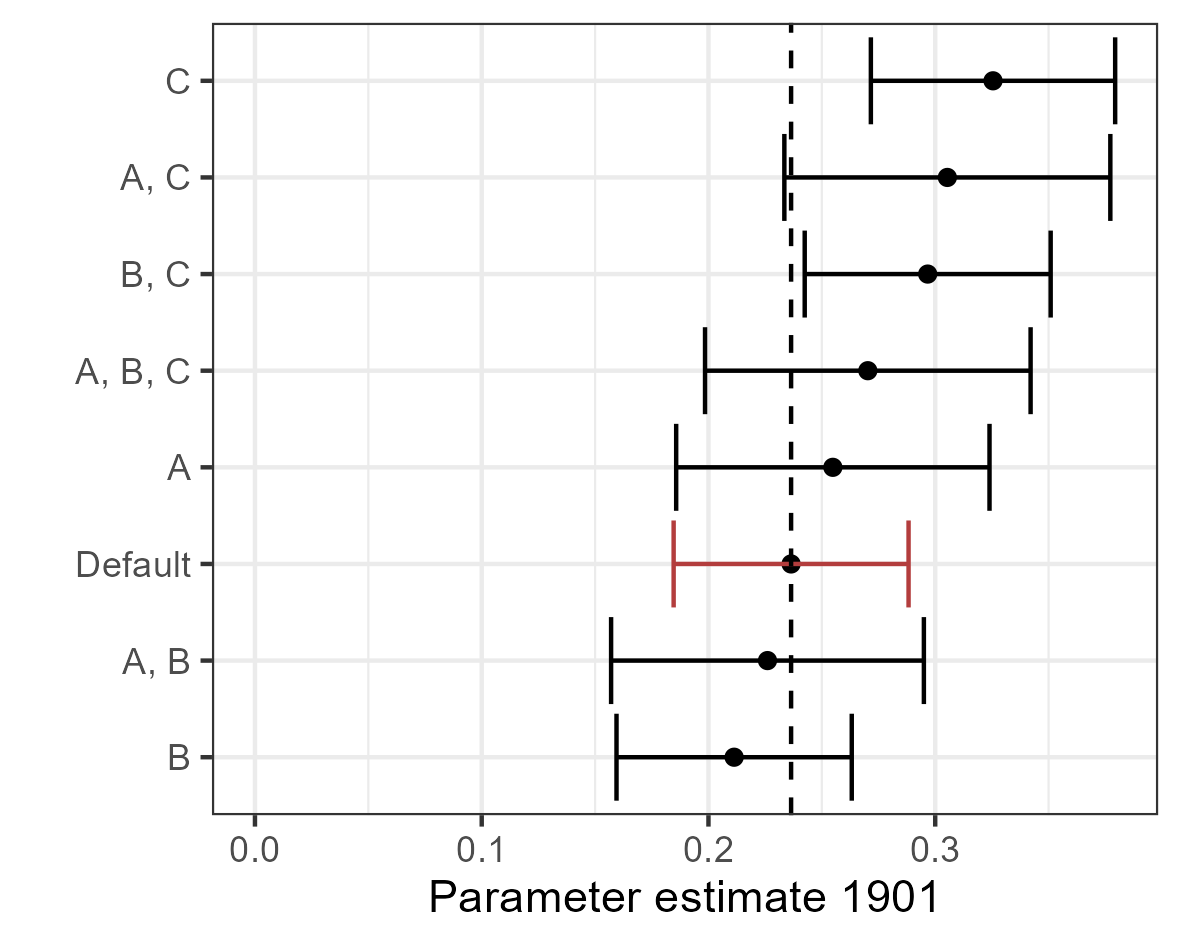
\includegraphics[width=\textwidth]{Plots/Regression_plots/Multiverse_dummy.png}
    \end{subfigure}
    \hfill
    \begin{subfigure}[b]{0.45\textwidth}
        \centering
        \caption{Multiverse of control groups\\Market access approach} \label{fig:mult2_1787}
        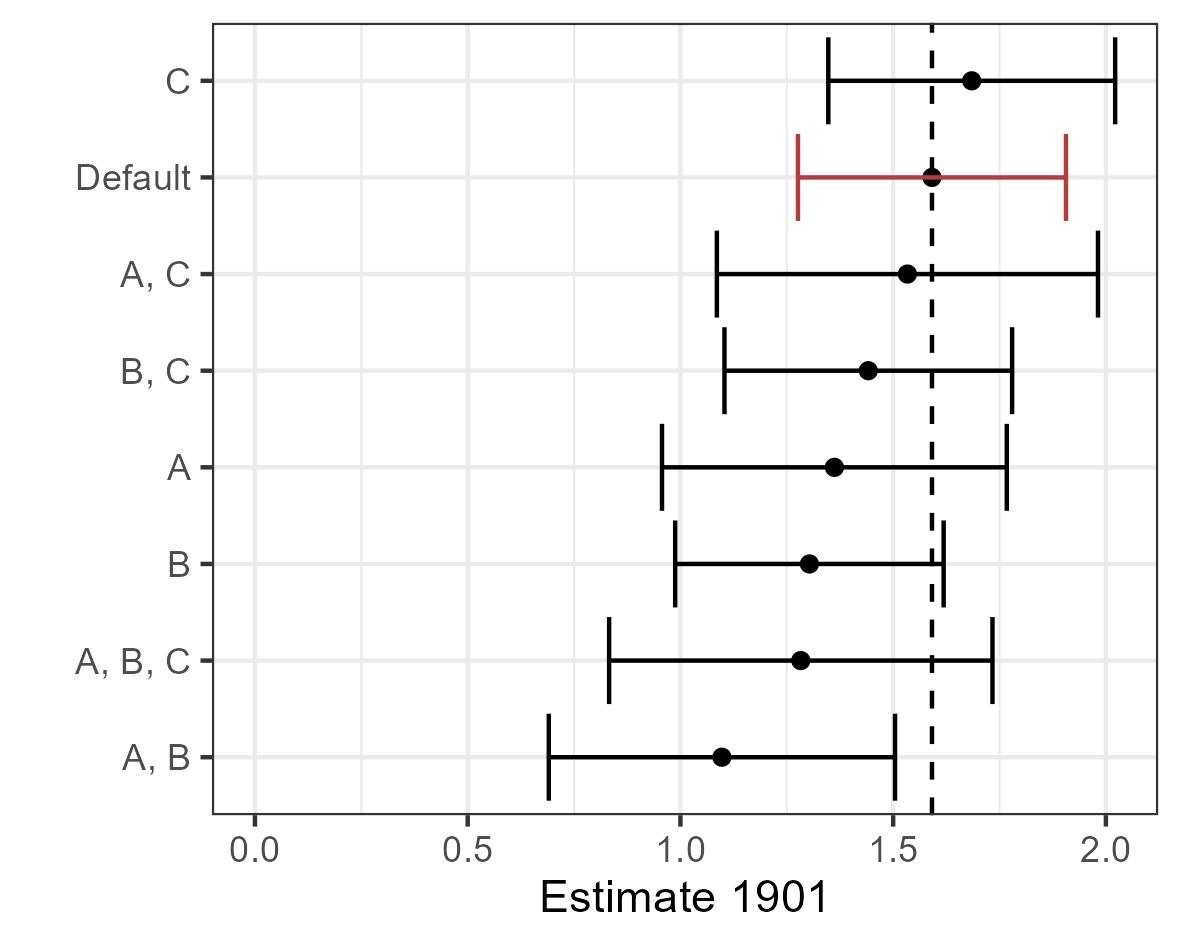
\includegraphics[width=\textwidth]{Plots/Regression_plots/Multiverse_MA.png}
    \end{subfigure}
    \vspace{0.45cm}
    \begin{subfigure}[b]{0.45\textwidth}
        \centering
        \caption{Multiverse of feasible parameters\\Market access approach} \label{fig:mult3_1787}
        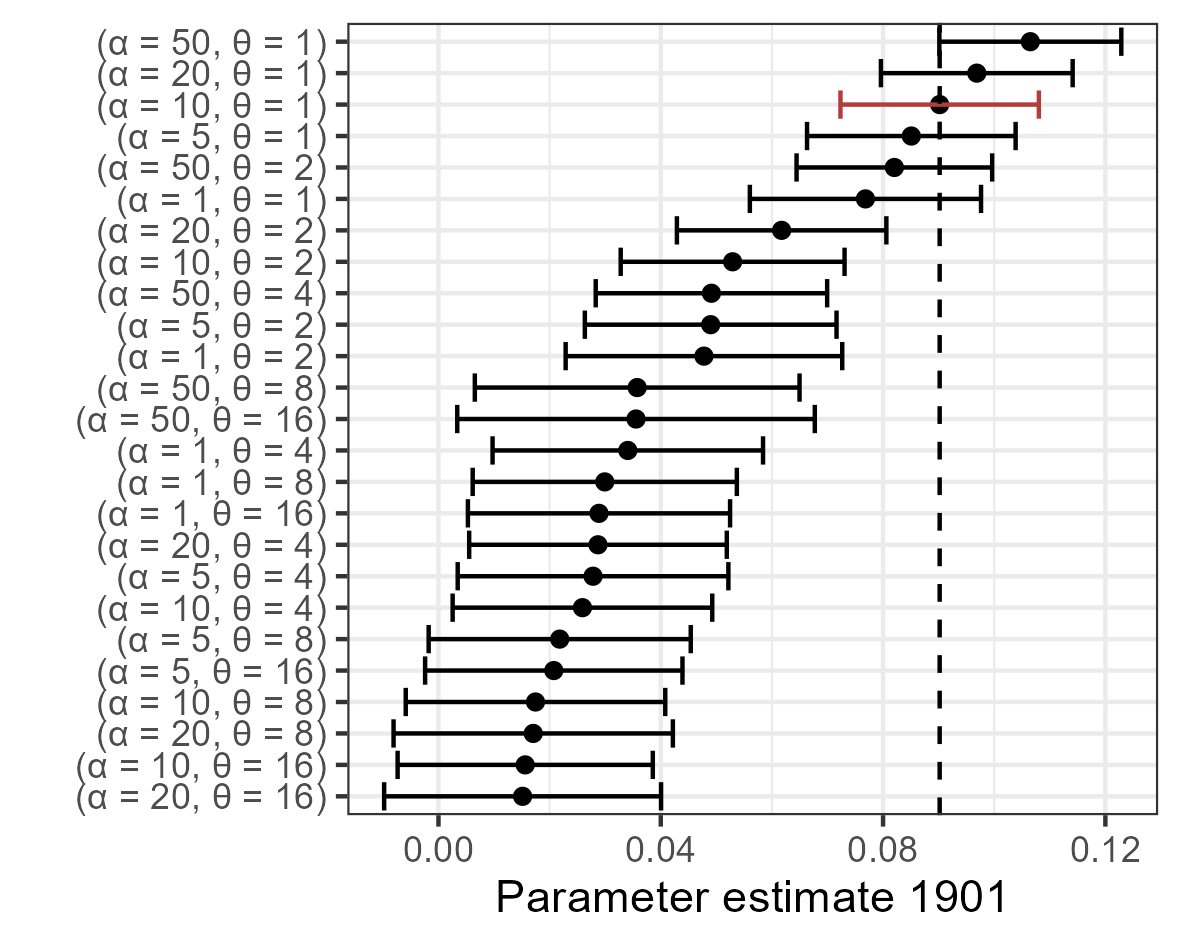
\includegraphics[width=\textwidth]{Plots/Regression_plots/Multiverse_MA_param.png}
    \end{subfigure}
    \parbox{0.9\textwidth}{
    \caption*{\footnotesize \textit{Notes:} This is the multiverse of parameter estimates of the effect in 1901 given different feasible choices that could have been made for how to run the analysis. In panel a and panel b, 'A', 'B', and 'C', represents subgroups of the data. 'A' is the result, when the regression is computed using only parishes with a centroid less than 5 km from the coast. 'B' is the subgroups, where all parishes in around Copenhagen are excluded, 'C' is the subgroup of parishes, where the control group does not contain any parishes within 100 km of the Limfjord. 'D' represents the result when using only parishes located within 5 km of a market town. Panel (c) represents the effect given different market access parameters. For enhanced comparability, the log change in market access is standardized to unit variance and zero mean. \\ \textit{Source: Danish census data}}
} \label{fig:pop2_1787}
\end{figure}

\begin{figure}[H]
    \centering
    \caption{Multiverse of the effect in different comparison groups and parameter choices}
    \begin{subfigure}[b]{0.45\textwidth}
        \centering
        \caption{Multiverse of control groups\\Dummy approach} \label{fig:mult1}
        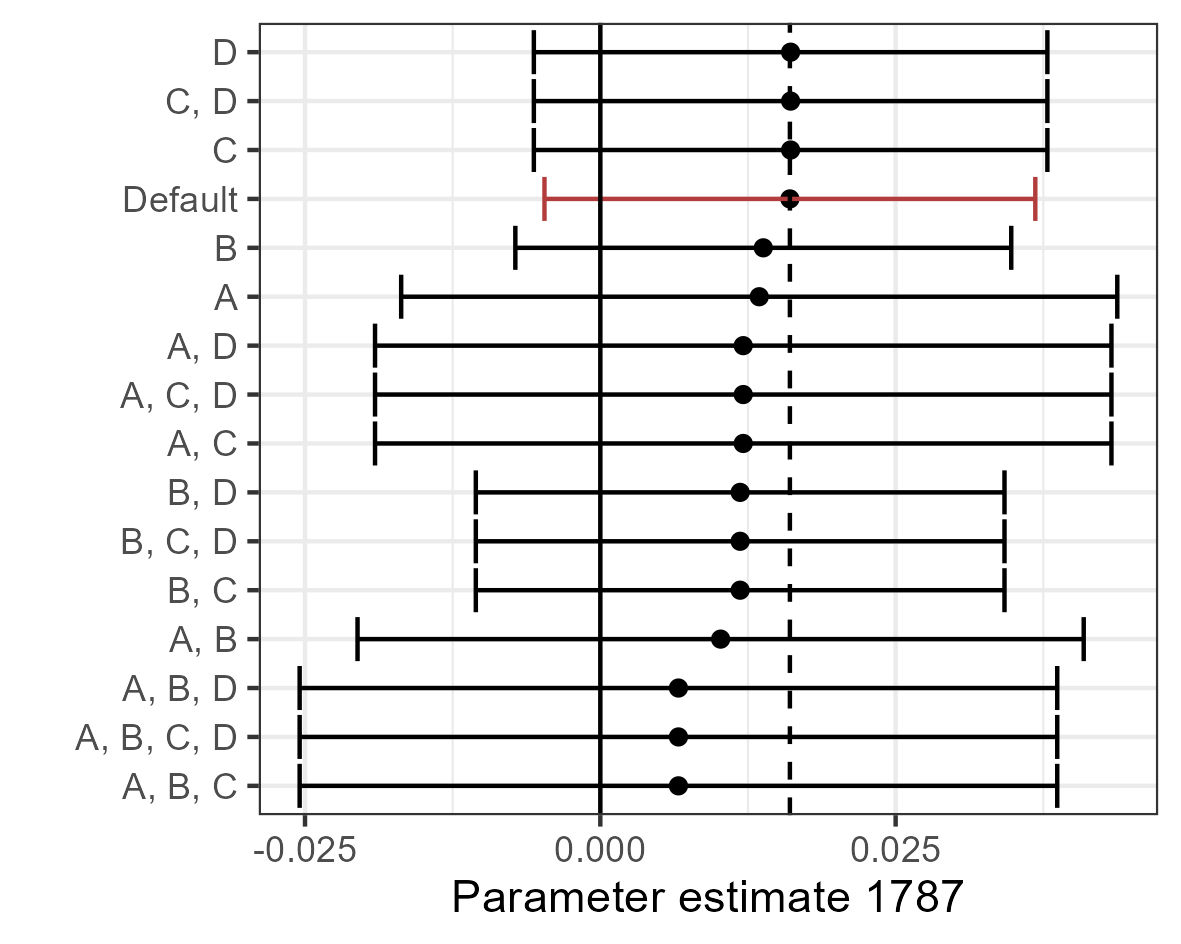
\includegraphics[width=\textwidth]{Plots/Regression_plots/Multiverse_dummy_1787.png}
    \end{subfigure}
    \hfill
    \begin{subfigure}[b]{0.45\textwidth}
        \centering
        \caption{Multiverse of control groups\\Market access approach} \label{fig:mult2}
        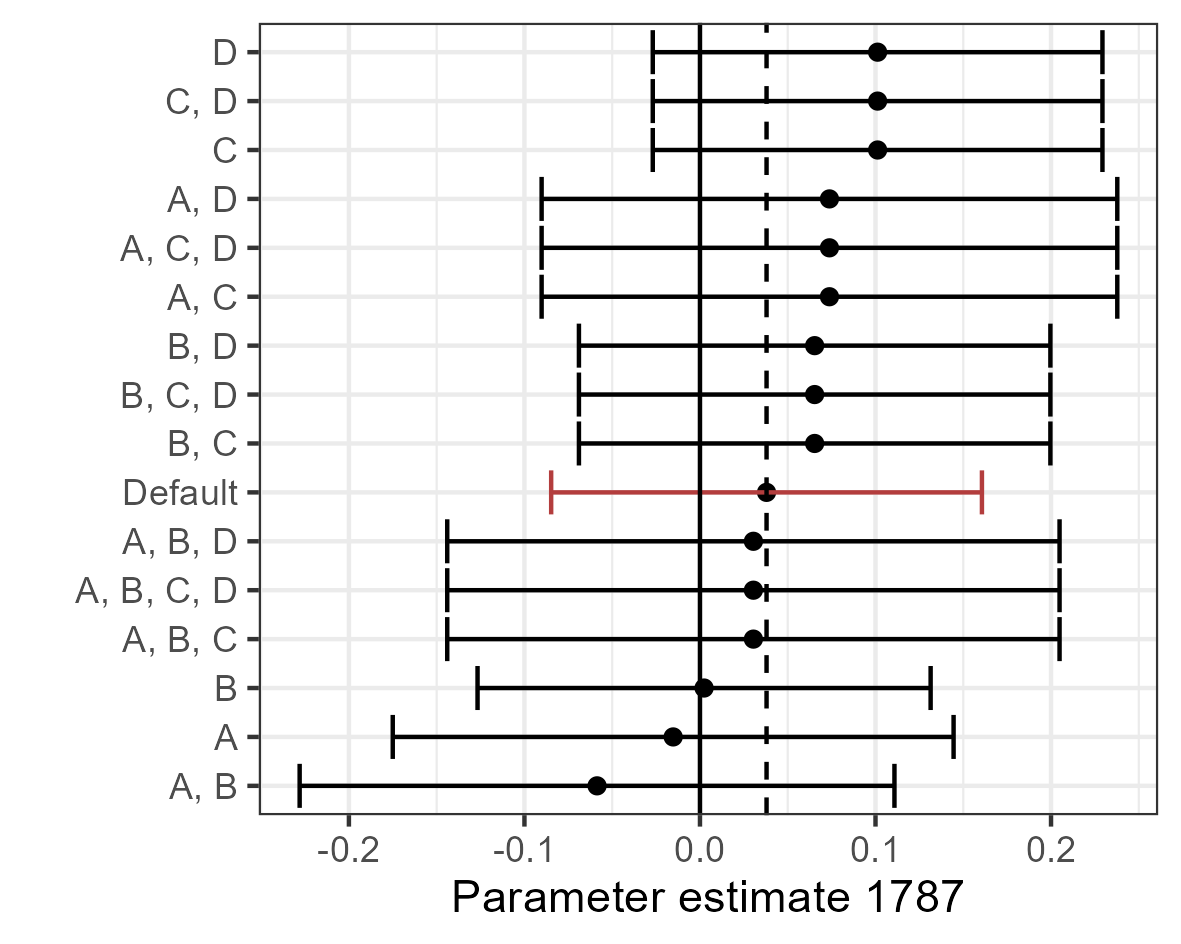
\includegraphics[width=\textwidth]{Plots/Regression_plots/Multiverse_MA_1787.png}
    \end{subfigure}
    \vspace{0.45cm}
    \begin{subfigure}[b]{0.45\textwidth}
        \centering
        \caption{Multiverse of feasible parameters\\Market access approach} \label{fig:mult3}
        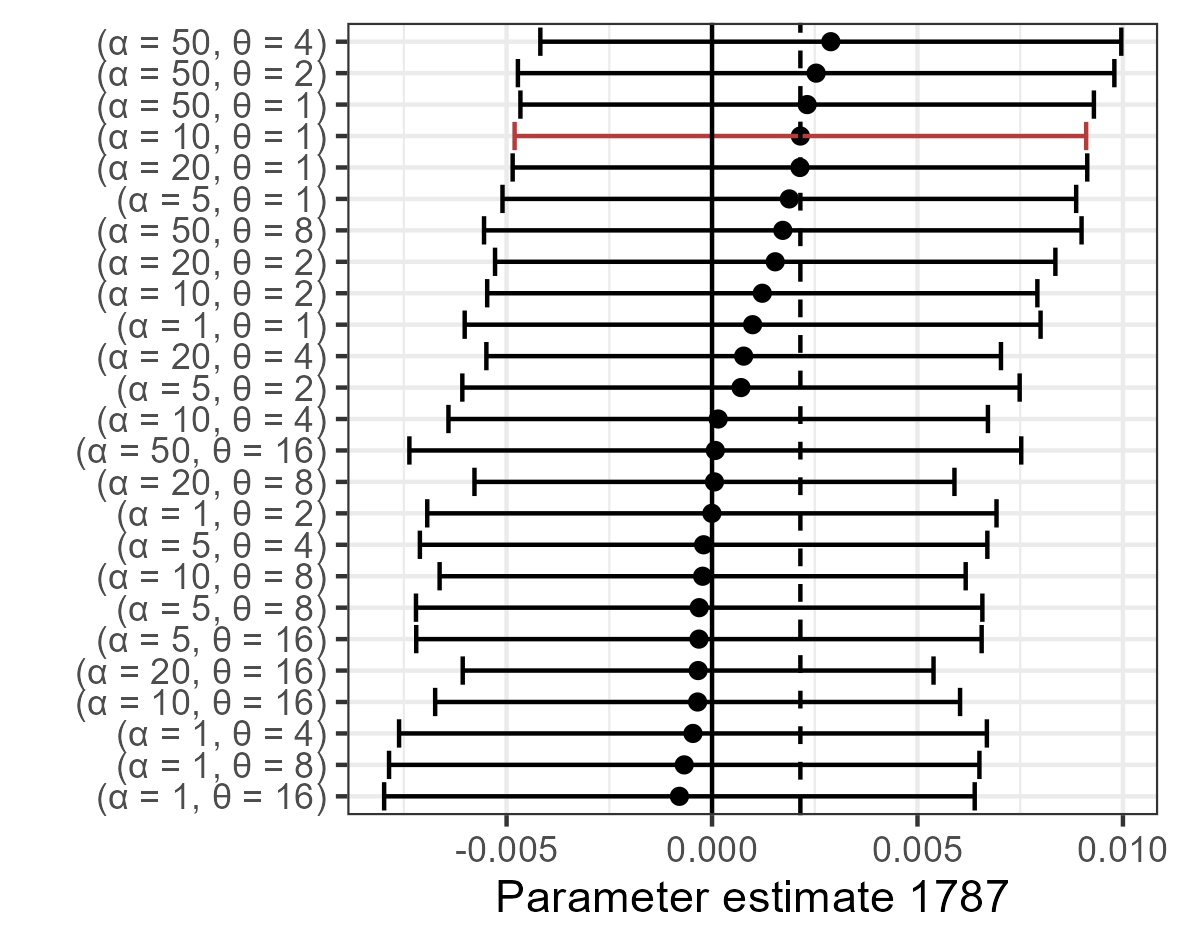
\includegraphics[width=\textwidth]{Plots/Regression_plots/Multiverse_MA_param_1787.png}
    \end{subfigure}
    \caption*{Notes: Multiverse results for 1787. If any of these were different from zero it would indicate the existence of pretends. The dotted line indicate the default parameter estimate. The solid line is at zero.}
    \label{fig:pop2}
\end{figure}

\FloatBarrier
\subsection{Doubly robust estimates}
This section contains estimates based on the doubly-robust multi-period did estimator from \cite{Callaway2021did}. Table \ref{tab:cs_estimates} shows the results. As is default in their implementation, the first period is the reference. As consequence, the reference year here is 1787 rather than 1801 from the rest of my paper. To address concern over balance, covariates are included. The doubly robust method combines a propensity score and an outcome regression and is consistent if either of these are correctly specified \citep{Santanna2020DRDID}. Column 1 shows results without covariates. Column 2 shows results including covariates (Occupation, Young children per woman and number of people in different age groups). Column 3 also includes the pre-event population as a covariate. 


\begin{table}[H]
\centering
\caption{Callaway and Sant'Anna estimates} \label{tab:cs_estimates}
\footnotesize
\begin{tabular}{lccc}
   \tabularnewline \midrule \midrule
   Outcome: & \multicolumn{3}{c}{log(Population)}\\
            & (1)           & (2)             & (3)\\  
   \midrule
    1801 & -0.0152      & -0.0273     & -0.0273 \\
         & (0.0114)     & (0.0141)    & (0.0133) \\
    1834 & 0.0221       & 0.0041      & 0.0041 \\
         & (0.0133)     & (0.0148)    & (0.0145) \\
    1840 & 0.0004       & -0.0097     & -0.0097 \\
         & (0.0132)     & (0.0154)    & (0.0145) \\
    1845 & 0.0031       & -0.0058     & -0.0058 \\
         & (0.0137)     & (0.0156)    & (0.0149) \\
    1850 & 0.0076       & -0.0040     & -0.0040 \\
         & (0.0146)     & (0.0174)    & (0.0160) \\
    1860 & 0.0343       & 0.0087      & 0.0087 \\
         & (0.0166)     & (0.0187)    & (0.0194) \\
    1880 & 0.1336*      & 0.0873*     & 0.0873* \\
         & (0.0198)     & (0.0229)    & (0.0233) \\
    1901 & 0.2262*      & 0.1590*     & 0.1590* \\
         & (0.0263)     & (0.0276)    & (0.0310)\\  
   \midrule
   Observations & 14,2741 & 14,274 & 14,274\\
   \midrule \midrule
   \multicolumn{4}{l}{\emph{'*' confidence band (95 percent) does not cover 0}}\\
\end{tabular}
\parbox{0.6\textwidth}{
\caption*{Notes: Effect using the estimator proposed by Callaway \& Sant’Anna (2021). Column (1) includes no covariates. Column (2) adjusts for pre-event covariates. Column (3) adjusts for pre-event covariates including pre-event population. \\ \textit{Source: Danish census data}}
}

\end{table}

\section{Mechanims}

\FloatBarrier
\subsection{All occupational major categories estimates} 

\begin{table}
    \centering
    \caption{Effect on occupation in 1901 (HISCO first digit 1 to 3)} \label{tab:occ1}
    \footnotesize
    \begin{tabular}{ccccc}
\toprule
hisco & Affected & Approach & Estimate (1901) & n parishes\\
\midrule
0/1 & MA & 3: log(x+1) & -0.642 (0.337) & 1589\\
0/1 & MA & 4: asinh(x) & -0.595 (0.397) & 1589\\
0/1 & MA & 1: Extensive & 0.414 (0.139) & 1589\\
0/1 & MA & 2: Intensive & -0.41 (0.445) & 1342\\
0/1 & Dummy & 3: log(x+1) & -0.083 (0.06) & 1589\\
0/1 & Dummy & 4: asinh(x) & -0.081 (0.07) & 1589\\
0/1 & Dummy & 1: Extensive & 0.064 (0.025) & 1589\\
0/1 & Dummy & 2: Intensive & -0.047 (0.079) & 1342\\
2 & MA & 3: log(x+1) & -0.871 (0.463) & 1589\\
2 & MA & 4: asinh(x) & -0.561 (0.521) & 1589\\
2 & MA & 1: Extensive & 0.182 (0.148) & 1589\\
2 & Dummy & 3: log(x+1) & -0.085 (0.085) & 1589\\
2 & Dummy & 2: Intensive & 0.081 (0.148) & 764\\
2 & Dummy & 4: asinh(x) & -0.056 (0.096) & 1589\\
2 & MA & 2: Intensive & 0.04 (0.761) & 764\\
2 & Dummy & 1: Extensive & -0.015 (0.025) & 1589\\
3 & MA & 2: Intensive & 1.962 (4.096) & 75\\
3 & Dummy & 2: Intensive & 1.252 (0.472) & 75\\
3 & MA & 1: Extensive & 1.128*** (0.259) & 1589\\
3 & MA & 4: asinh(x) & 0.697 (0.479) & 1589\\
3 & MA & 3: log(x+1) & 0.486 (0.381) & 1589\\
3 & Dummy & 1: Extensive & 0.169*** (0.044) & 1589\\
3 & Dummy & 4: asinh(x) & 0.101 (0.087) & 1589\\
3 & Dummy & 3: log(x+1) & 0.073 (0.07) & 1589\\
\bottomrule
\end{tabular}
\parbox{0.9\textwidth}{
\caption*{\footnotesize \textit{Notes:} Parameter estimate of the effect on occupational structure of the channel in 1901. Each row corresponds to a sepperate regression with all individuals with hisco codes starting with 0/1, 2 or 3 as outcome. The last column shows the number of parishes included in the regression, which is different from the full sample (1589) in the intensive margin estimates. As a rule of thumb, results with fewer than 100 observations should be entirely disregarded. *** $p< 0.01$ ** $p< 0.05$ * $p< 0.10$. Standard errors clustered on the parish level in parenthesis. All p-values are Bonferroni-corrected. \\ \textit{Source:} Danish census data.}
}
\end{table}

\begin{table}
    \centering
    \caption{Effect on occupation in 1901 (HISCO first digit 4 to 9)} \label{tab:occ2}
    \footnotesize
    \begin{tabular}{ccccc}
\toprule
hisco & Affected & Approach & Estimate (1901) & n parishes\\
\midrule
4 & MA & 2: Intensive & -4.772 (3.826) & 28\\
4 & MA & 4: asinh(x) & -1.342 (0.576) & 1589\\
4 & MA & 3: log(x+1) & -1.121 (0.489) & 1589\\
4 & Dummy & 2: Intensive & -0.353 (0.402) & 28\\
4 & Dummy & 4: asinh(x) & -0.182 (0.103) & 1589\\
4 & Dummy & 3: log(x+1) & -0.143 (0.087) & 1589\\
4 & MA & 1: Extensive & -0.123 (0.202) & 1589\\
4 & Dummy & 1: Extensive & -0.058 (0.036) & 1589\\
5 & MA & 4: asinh(x) & -0.943 (0.554) & 1589\\
5 & MA & 1: Extensive & -0.662*** (0.163) & 1589\\
5 & MA & 3: log(x+1) & -0.625 (0.462) & 1589\\
5 & Dummy & 2: Intensive & 0.309 (0.159) & 660\\
5 & MA & 2: Intensive & 0.302 (0.881) & 660\\
5 & Dummy & 3: log(x+1) & 0.057 (0.079) & 1589\\
5 & Dummy & 4: asinh(x) & 0.042 (0.094) & 1589\\
5 & Dummy & 1: Extensive & -0.031 (0.028) & 1589\\
6 & MA & 2: Intensive & 1.173*** (0.196) & 1545\\
6 & MA & 1: Extensive & -0.243*** (0.049) & 1589\\
6 & Dummy & 2: Intensive & 0.197*** (0.031) & 1545\\
6 & MA & 4: asinh(x) & -0.123 (0.322) & 1589\\
6 & Dummy & 3: log(x+1) & 0.085 (0.036) & 1589\\
6 & Dummy & 4: asinh(x) & 0.072 (0.038) & 1589\\
6 & MA & 3: log(x+1) & 0.025 (0.294) & 1589\\
6 & Dummy & 1: Extensive & -0.024*** (0.004) & 1589\\
7/8/9 & MA & 2: Intensive & 1.763*** (0.339) & 1530\\
7/8/9 & MA & 4: asinh(x) & 0.813 (0.39) & 1589\\
7/8/9 & MA & 3: log(x+1) & 0.709 (0.358) & 1589\\
7/8/9 & MA & 1: Extensive & -0.218*** (0.05) & 1589\\
7/8/9 & Dummy & 2: Intensive & 0.215** (0.063) & 1530\\
7/8/9 & Dummy & 4: asinh(x) & 0.123 (0.068) & 1589\\
7/8/9 & Dummy & 3: log(x+1) & 0.11 (0.063) & 1589\\
7/8/9 & Dummy & 1: Extensive & -0.02 (0.007) & 1589\\
\bottomrule
\end{tabular}
\parbox{0.9\textwidth}{
\caption*{\footnotesize \textit{Notes:} Parameter estimate of the effect on occupational structure of the channel in 1901. Each row corresponds to a sepperate regression with all individuals with hisco codes starting with 4, 5, or 6/8/9 as outcome. The last column shows the number of parishes included in the regression, which is different from the full sample (1589) in the intensive margin estimates. As a rule of thumb, results with fewer than 100 observations should be entirely disregarded. *** $p< 0.01$ ** $p< 0.05$ * $p< 0.10$. Standard errors clustered on the parish level in parenthesis. All p-values are Bonferroni-corrected. \\ \textit{Source:} Danish census data.}
}
\end{table}

\FloatBarrier

\subsection{Event plot fishing and spinning}
\begin{figure}
    \centering
    \caption{Fishermen and Spinners, Weavers, Knitters, Dyers And Related Workers}
    \begin{subfigure}[b]{0.45\textwidth}
        \centering
        \caption{Fishermen (MA approach)} \label{fig:fish_ma}
        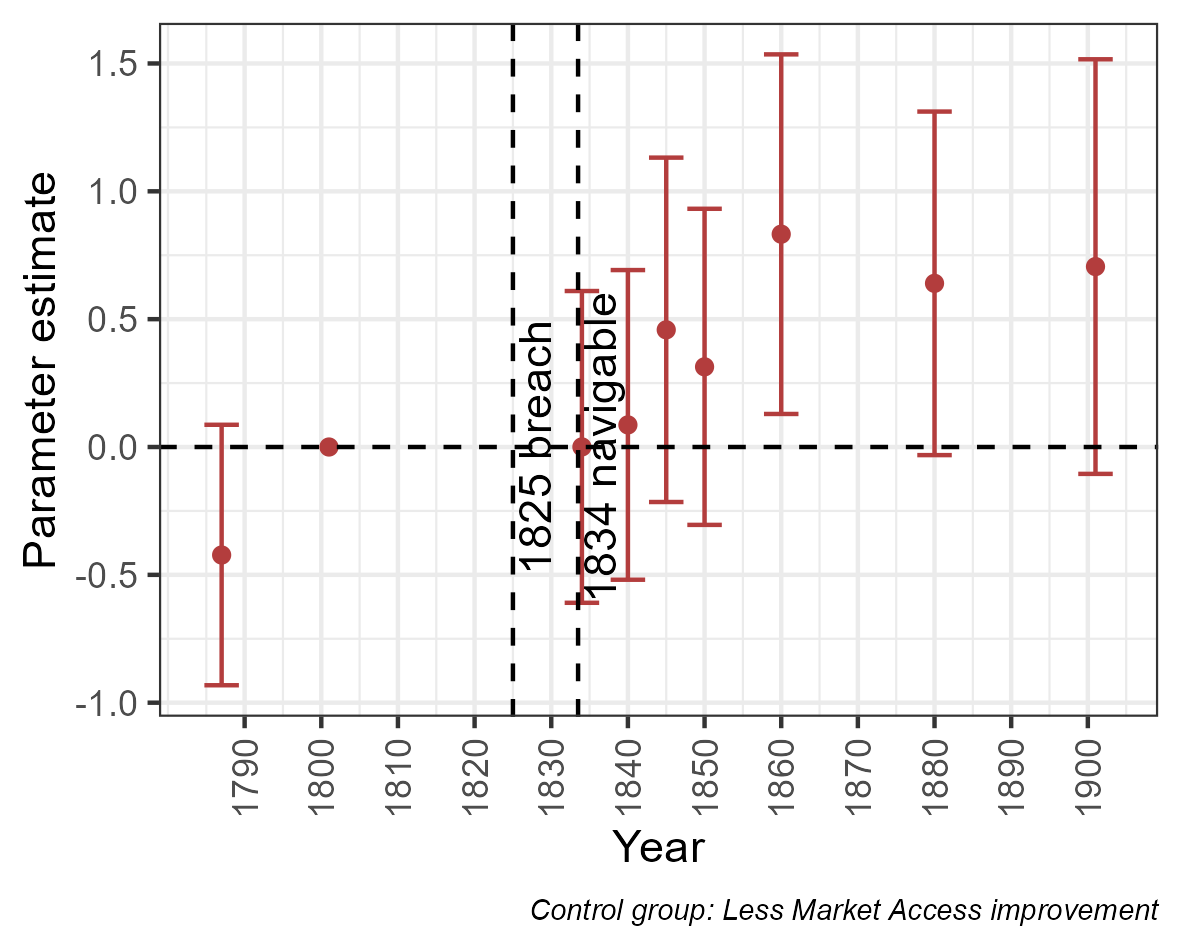
\includegraphics[width=\textwidth]{Plots/Mechanism/fish_MA.png}
    \end{subfigure}
    \hfill
    \begin{subfigure}[b]{0.45\textwidth}
        \centering
        \caption{Fishermen (Dummy approach)} \label{fig:fish_dummy}
        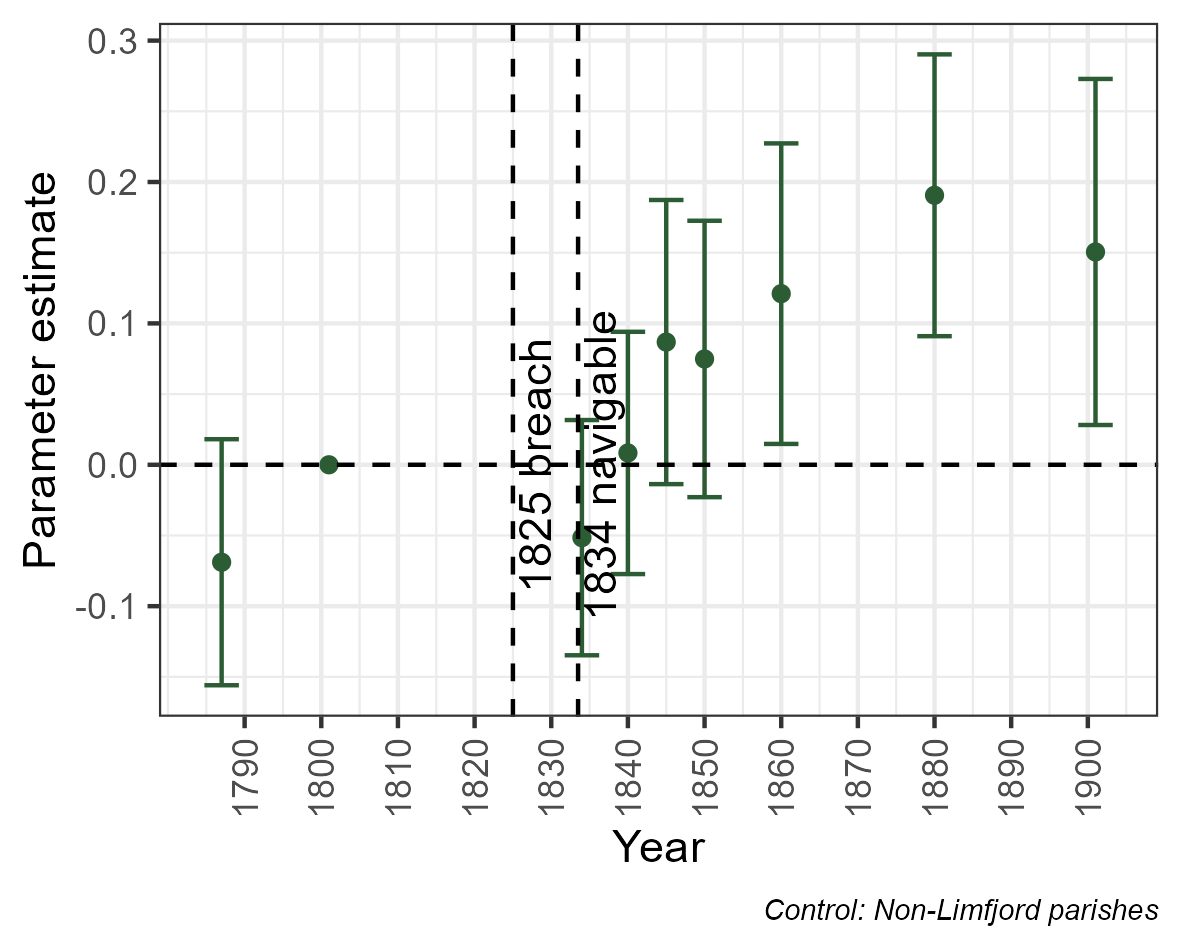
\includegraphics[width=\textwidth]{Plots/Mechanism/fish_dummy.png}
    \end{subfigure}
    \vspace{0.45cm}
    \begin{subfigure}[b]{0.45\textwidth}
        \centering
        \caption{Spinners, weavers, knitters, dyers and related workers (MA approach)} \label{fig:spinners_ma}
        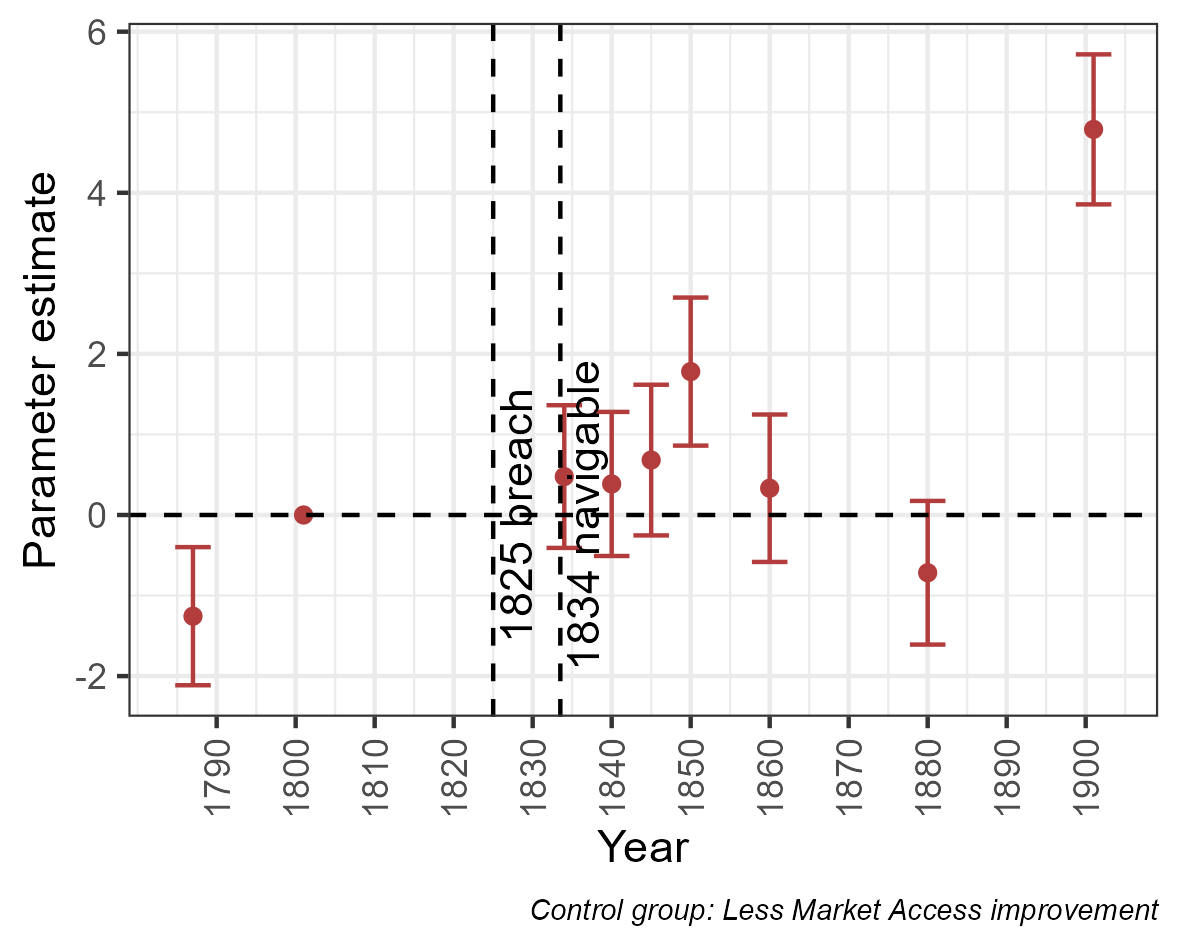
\includegraphics[width=\textwidth]{Plots/Mechanism/spinning_MA.png}
    \end{subfigure}
    \hfill
    \begin{subfigure}[b]{0.45\textwidth}
        \centering
        \caption{Spinners, weavers, knitters, dyers and related workers (Dummy approach)} \label{fig:spinners_dummy}
        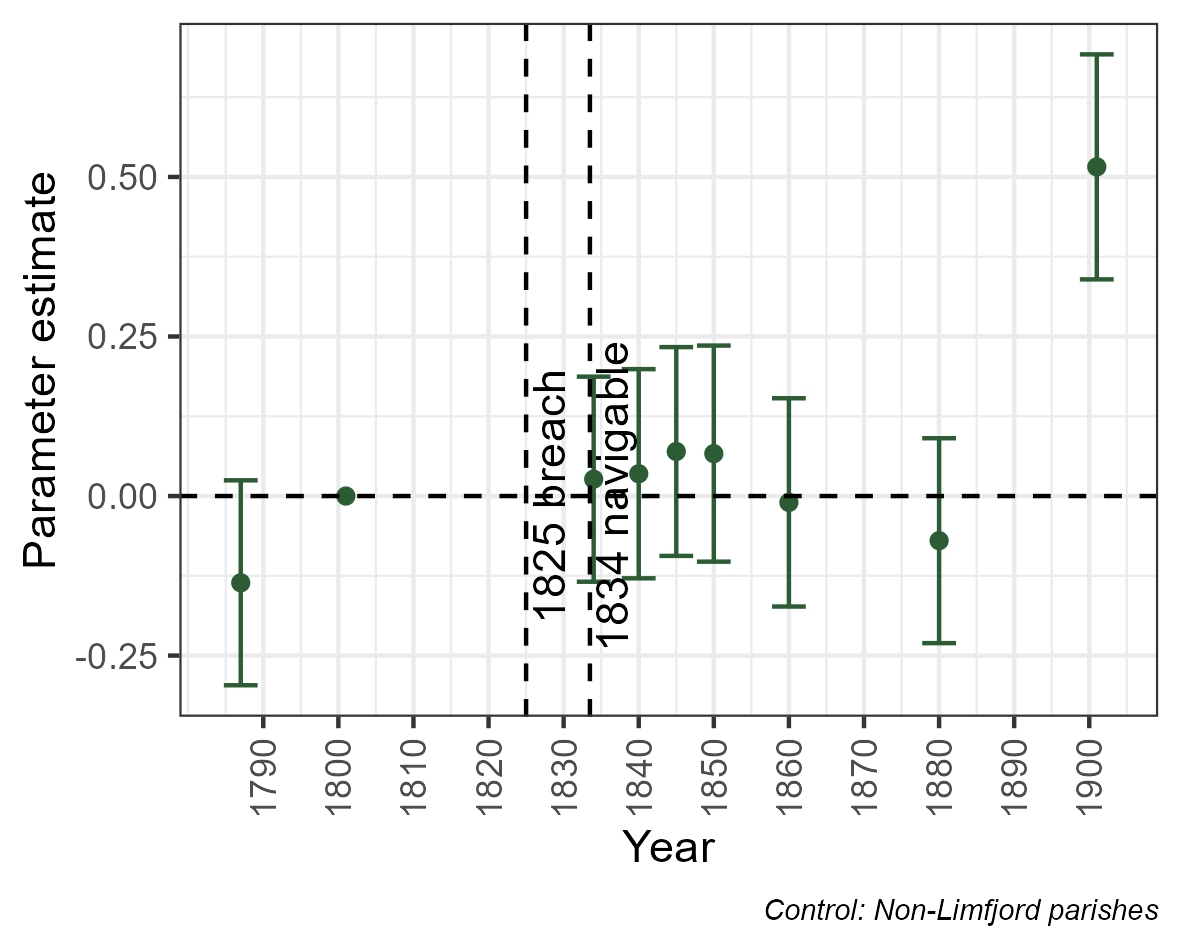
\includegraphics[width=\textwidth]{Plots/Mechanism/spinning_dummy.png}
    \end{subfigure}
    \parbox{0.9\textwidth}{
    \caption*{\footnotesize \textit{Notes:} Panel (a) and panel (b) shows event plots for the effect of the channel on the number of fishermen. Panel (c) and (d) shows the effect to the number of spinners, weavers, knitters, dyers and related workers (HISCO codes starting with 75).  \\ \textit{Source: Danish census data}}
}
    \label{fig:fishing_spinners}
\end{figure}

\FloatBarrier
\subsection{Effects by age group} 
\begin{figure}
    \centering
    \caption{Age group composition}
    \begin{subfigure}[b]{0.45\textwidth}
        \centering
        \caption{Effect by age group (MA approach)} \label{fig:migr}
        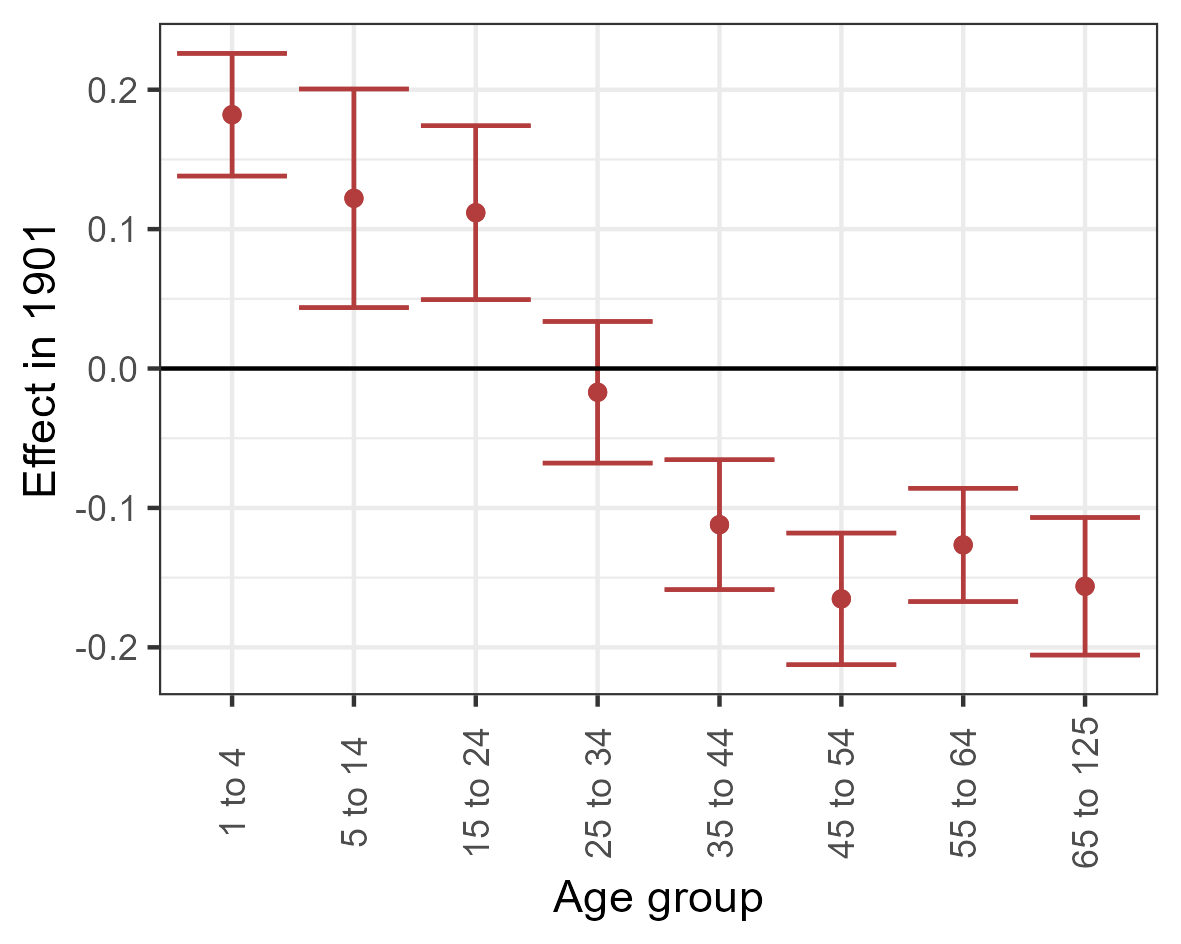
\includegraphics[width=\textwidth]{Plots/Mechanism/Age_composition_MA.png}
    \end{subfigure}
    \hfill
    \begin{subfigure}[b]{0.45\textwidth}
        \centering
        \caption{Effect by age group (dummy approach)} \label{fig:fert}
        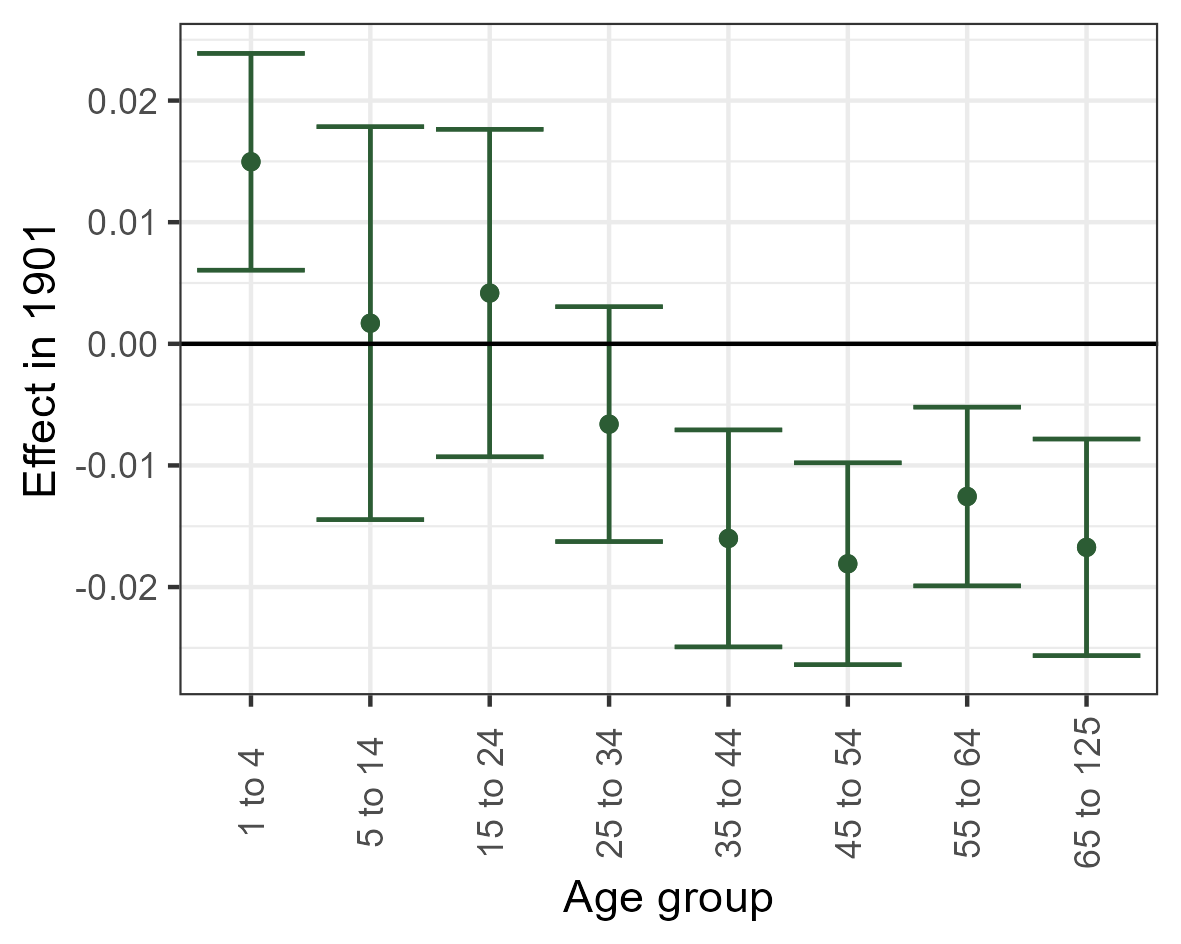
\includegraphics[width=\textwidth]{Plots/Mechanism/Age_composition_Dummy.png}
    \end{subfigure}
    \parbox{0.9\textwidth}{
    \caption*{\footnotesize \textit{Notes:} Regression parameter in 1901 given the market access approach (panel a) and the dummy approach (panel b). The outcome of each regression is the size of the particular age group as a share of the total population. What this shows, is that the population in the affected parishes became comparatively younger.  \\ \textit{Source: Danish census data}}
}
    \label{fig:age_group}
\end{figure}

\FloatBarrier
\section{Archaeological findings}

\subsection{Math note} 
The derivation is based on a single parish $i$. To construct a panel this is simply repeated for all parishes. The derivation is based on coin findings. But it generalises to any kind of finding.    

The data is of the form: $Coin=c$ was generated in time interval $t\in [Y_{min}^c;Y_{max}^c]$ (Archaeologists report a coin finding and date it to a range.)

That is, for each coin we observe $P(t|c)\sim [Y_{min}^c;Y_{max}^c]$ 

We want to know the probability, that any coin, $c\in \{1, ..., K\}$, finding was generated at any particular point in time. This event is referred to as $\{coins\}|t$

\subsubsection{Probability of a single coin} 
We are interested in the probability that a any coin comes from a specific point in time. What is observed is:

\begin{equation}
P(t|c)=\begin{cases}
\frac{1}{Y_{max}^c - Y_{min}^c}, & \text{if }Y_{min}^c\leq t \leq Y_{max}^c \\
0 & \text{otherwise}
\end{cases}
\end{equation}

Or writing the same with indicator function:

\begin{equation}
P(t|c)=1[t\in [Y_{min}^c;Y_{max}^c]]\frac{1}{Y_{max}^c - Y_{min}^c}
\end{equation}

I.e. it is equally likely that a coin truly originates at any particular point in time the range offered by the archaeologists. 

**Note:**
This is an assumption. The archaeologists specify a range but not a distribution. How should this range be interpreted? A straightforward alternative is to intepret it as a 95 percent confidence interval of the normal distribution. This is also tested. 

\begin{equation}
\begin{split}
P(t|c)&=\mathcal{N}(\mu_c,\sigma_c)\\
\text{where:} \\
\mu_c&=0.5\times(Y_{max}^c + Y_{min}^c)\\
\sigma_c&\approx(Y_{max}^c - Y_{min}^c)/1.96
\end{split}
\end{equation}

\subsubsection{At the parish level}
The probability that *any* coin was generated as a finding in the parish (at least one of the draws from $P(t|c)$ was succesful) is a mixture distribution, where at least one component needs to be sucesful:

\begin{equation}
\begin{split}
P(t|\{coins\})&=1-\prod_{c=1}^K \left( 1 - P(t|c) \right) \\
P(t|\{coins\})&=1-\prod_{c=1}^K \left(1 - 1[t\in [Y_{min}^c;Y_{max}^c]] \left(\frac{1}{Y_{max}^c - Y_{min}^c}\right) \right)
\end{split}
\end{equation}

where $\{coins\}$ is the event of at least one coin $\{coins\}=\{1,...,c,...,K\}$. 

*Intuition*
The inner part of the expression ($1 - P(t|c)$) is the probability that a coin is *not* associated with that particular point in time. Taking the product over all coins, generates the combined probability, that *no coins at all* are associated with that particular point in time. The compliment of this is the probability we are interested in, in this step. It is the probability that *any* coin is associated with a particular point in time. 

\subsubsection{Reverse probability} 
We are interested in the reverse probability: The probability of any coins given a particular point in time. The formula for this is Bayes formula:

\begin{equation}
P(\{coins\}|t) = \frac{P(t|\{coins\})P(\{coins\})}{P(t)}
\end{equation}

The prior, $P(\{coins\})$, is simply assumed to be a constant, $0<c<1$ and $P(t)$ can be found by marginalisation  $P(t)=P(t|\{coins\})+P(t|\neg\{coins\})=1$. It follows that

\begin{equation}
P(\{coins\}|t) = c\times P(t|\{coins\})
\end{equation}

\subsubsection{Estimation}
The following loop (pseudocode) produces samples from $P(\{coins\}|t)$ and estimates the probability of interest:

\begin{verbatim}
    ```{pseudo code}
    B = 1000 # Number of Monte Carlo samples
    
    for b in 1 to B: # Loop of MC samples
    ...	# Generate samples from Y_max_c Y_max_c:
    ...	for c in 1 to C:
    ...	...	t_c = sample_uniform(1, Y_min_c, Y_max_c)
    ...	...	# Is t_c equal to t?
    ...	...	coins_t[c] = t_c == t
    		
    ...	# Were there any coins associated with this time in this draw?
    ...	number_of_coins = sum(coins_t)
    ...	succces_t[b] = number_of_coins > 0
    	
    # Estimating the probability by analogy for each t
    P_of_t_given_coins = sum(succces_t) / B
    
    # Converting to P({coins}|t)
    P_of_coins_given_t = c_hat * P_of_t_given_coins
    ```
\end{verbatim}



This code is then repeated for every parish and every point in time $t$. This gives a panel of size $N\times T$ containing the estimated probability that a coin finding was generated at a particular point in time. This in turn can be used in econometric applications. 

\newpage
\subsection{All parameter estimates}
Table \ref{tab:A_arch1} and \ref{tab:A_arch2} contain parameter estimates for all years for the regressions using archaeological findings. 

\begin{table}[H]
\centering
\footnotesize
\caption{All parameters of table 3 columns 1-4} \label{tab:A_arch1}
\begin{tabular}{lcccc}
   \tabularnewline \midrule \midrule
                                                    & \multicolumn{4}{c}{Archaeological findings}\\
                                                    & (1)             & (2)             & (3)                   & (4)\\  
                                                    & MA              & Dummy           & MA                    & Dummy\\
   \midrule
   Year750 $\times$ Affected                        & 0.0521$^{***}$  & 0.0050$^{***}$  & 0.0034                & -0.0010\\   
                                                    & (0.0092)        & (0.0009)        & (0.0101)              & (0.0018)\\   
   Year800 $\times$ Affected                        & 0.0195$^{***}$  & 0.0020$^{***}$  & -0.0060               & -0.0024$^{*}$\\   
                                                    & (0.0049)        & (0.0005)        & (0.0068)              & (0.0013)\\   
   Year850 $\times$ Affected                        & 0.0220$^{***}$  & 0.0022$^{***}$  & -0.0072               & -0.0028$^{**}$\\   
                                                    & (0.0051)        & (0.0006)        & (0.0068)              & (0.0013)\\   
   Year900 $\times$ Affected                        & 0.0086$^{**}$   & 0.0010$^{***}$  & -0.0031               & -0.0014$^{*}$\\   
                                                    & (0.0035)        & (0.0004)        & (0.0041)              & (0.0008)\\   
   Year950 $\times$ Affected                        & -0.0042         & -0.0002         & 0.0011                & 0.0002\\   
                                                    & (0.0038)        & (0.0004)        & (0.0018)              & (0.0003)\\   
   Year1050 $\times$ Affected                       & 0.0059$^{**}$   & 0.0008$^{***}$  & -0.0063$^{**}$        & -0.0007\\   
                                                    & (0.0025)        & (0.0003)        & (0.0032)              & (0.0006)\\   
   Year1100 $\times$ Affected                       & 0.0077          & 0.0004          & -0.0708$^{***}$       & -0.0066$^{**}$\\   
                                                    & (0.0121)        & (0.0011)        & (0.0165)              & (0.0032)\\   
   Year1150 $\times$ Affected                       & 0.0075          & 0.0003          & -0.0681$^{***}$       & -0.0065$^{*}$\\   
                                                    & (0.0121)        & (0.0011)        & (0.0170)              & (0.0033)\\   
   Year1200 $\times$ Affected                       & -0.0327$^{**}$  & -0.0049$^{***}$ & -0.0736$^{***}$       & -0.0069$^{**}$\\   
                                                    & (0.0151)        & (0.0013)        & (0.0174)              & (0.0034)\\   
   Year1250 $\times$ Affected                       & -0.0941$^{***}$ & -0.0120$^{***}$ & -0.0772$^{***}$       & -0.0066$^{*}$\\   
                                                    & (0.0199)        & (0.0018)        & (0.0193)              & (0.0038)\\   
   Year1300 $\times$ Affected                       & -0.1479$^{***}$ & -0.0147$^{***}$ & -0.0685$^{***}$       & -0.0068$^{**}$\\   
                                                    & (0.0236)        & (0.0032)        & (0.0178)              & (0.0031)\\   
   Year1350 $\times$ Affected                       & -0.1923$^{***}$ & -0.0193$^{***}$ & -0.0612$^{***}$       & -0.0065$^{**}$\\   
                                                    & (0.0273)        & (0.0037)        & (0.0185)              & (0.0031)\\   
   Year1400 $\times$ Affected                       & -0.1207$^{***}$ & -0.0116$^{***}$ & -0.0605$^{***}$       & -0.0060$^{**}$\\   
                                                    & (0.0239)        & (0.0034)        & (0.0177)              & (0.0030)\\   
   Year1450 $\times$ Affected                       & -0.0606$^{***}$ & -0.0052         & -0.0599$^{***}$       & -0.0060$^{**}$\\   
                                                    & (0.0234)        & (0.0034)        & (0.0174)              & (0.0029)\\   
   Year1500 $\times$ Affected                       & -0.1114$^{***}$ & -0.0104$^{***}$ & -0.0666$^{***}$       & -0.0064$^{*}$\\   
                                                    & (0.0256)        & (0.0037)        & (0.0223)              & (0.0035)\\   
   \midrule \midrule
   \multicolumn{5}{l}{\emph{Custom standard-errors in parentheses}}\\
   \multicolumn{5}{l}{\emph{Signif. Codes: ***: 0.01, **: 0.05, *: 0.1}}\\
\end{tabular}
\end{table}


\begin{table}
\centering
\footnotesize
\caption{All parameters of table 3 columns 5-8} \label{tab:A_arch2}
\begin{tabular}{lcccc}
   \tabularnewline \midrule \midrule
                                                    & \multicolumn{4}{c}{Archaeological findings}\\
                                                    & (5)             & (6)             & (7)                   & (8)\\  
                                                    & MA              & Dummy           & MA                    & Dummy\\
   \midrule
   Year750 $\times$ Affected   & 0.0547$^{**}$   & 0.0063$^{**}$   & -0.0043         & -0.0003\\   
                               & (0.0216)        & (0.0025)        & (0.0168)        & (0.0026)\\   
   Year800 $\times$ Affected   & 0.0261$^{**}$   & 0.0031$^{**}$   & -0.0248$^{*}$   & -0.0034\\   
                               & (0.0122)        & (0.0015)        & (0.0136)        & (0.0021)\\   
   Year850 $\times$ Affected   & 0.0231$^{*}$    & 0.0027$^{*}$    & -0.0306$^{**}$  & -0.0049$^{**}$\\   
                               & (0.0118)        & (0.0015)        & (0.0137)        & (0.0021)\\   
   Year900 $\times$ Affected   & 0.0071          & 0.0008          & -0.0199$^{**}$  & -0.0033$^{**}$\\   
                               & (0.0069)        & (0.0009)        & (0.0097)        & (0.0016)\\   
   Year950 $\times$ Affected   & -0.0177$^{*}$   & -0.0021$^{*}$   & 0.0008          & $-8.62\times 10^{-6}$\\    
                               & (0.0096)        & (0.0011)        & (0.0039)        & (0.0006)\\   
   Year1050 $\times$ Affected  & 0.0051          & 0.0006          & -0.0083         & -0.0012\\   
                               & (0.0039)        & (0.0005)        & (0.0064)        & (0.0010)\\   
   Year1100 $\times$ Affected  & 0.0309          & 0.0036          & -0.0700$^{**}$  & -0.0077\\   
                               & (0.0245)        & (0.0028)        & (0.0310)        & (0.0050)\\   
   Year1150 $\times$ Affected  & 0.0320          & 0.0036          & -0.0705$^{**}$  & -0.0078\\   
                               & (0.0245)        & (0.0029)        & (0.0318)        & (0.0051)\\   
   Year1200 $\times$ Affected  & -0.0338         & -0.0044         & -0.0736$^{**}$  & -0.0082\\   
                               & (0.0254)        & (0.0031)        & (0.0293)        & (0.0050)\\   
   Year1250 $\times$ Affected  & -0.1216$^{***}$ & -0.0150$^{***}$ & -0.0829$^{***}$ & -0.0093$^{*}$\\   
                               & (0.0350)        & (0.0045)        & (0.0318)        & (0.0054)\\   
   Year1300 $\times$ Affected  & -0.1280$^{***}$ & -0.0131$^{**}$  & -0.0828$^{***}$ & -0.0099$^{**}$\\   
                               & (0.0379)        & (0.0052)        & (0.0294)        & (0.0047)\\   
   Year1350 $\times$ Affected  & -0.1408$^{***}$ & -0.0159$^{***}$ & -0.0669$^{**}$  & -0.0076\\   
                               & (0.0414)        & (0.0058)        & (0.0297)        & (0.0046)\\   
   Year1400 $\times$ Affected  & -0.0962$^{**}$  & -0.0104$^{*}$   & -0.0682$^{**}$  & -0.0077$^{*}$\\   
                               & (0.0422)        & (0.0058)        & (0.0287)        & (0.0046)\\   
   Year1450 $\times$ Affected  & -0.0693         & -0.0068         & -0.0717$^{**}$  & -0.0082$^{*}$\\   
                               & (0.0466)        & (0.0064)        & (0.0293)        & (0.0047)\\   
   Year1500 $\times$ Affected  & -0.1069$^{**}$  & -0.0121$^{*}$   & -0.0511         & -0.0066\\   
                               & (0.0513)        & (0.0071)        & (0.0362)        & (0.0052)\\   
   \midrule \midrule
   \multicolumn{5}{l}{\emph{Custom standard-errors in parentheses}}\\
   \multicolumn{5}{l}{\emph{Signif. Codes: ***: 0.01, **: 0.05, *: 0.1}}\\
\end{tabular}
\end{table}

\FloatBarrier
\subsection{Normal distribution}
Figure \ref{fig:arch_reg1}, \ref{fig:arch_reg_boot1}, \ref{fig:arch_reg2} and \ref{fig:arch_reg_boot2} show equivalent results to those presented in the paper. However, these are results based on assuming that the archaeological datings (e.g. coin finding dated to the years 1300-1495) represent a 95 percent confidence interval from a normal distribution rather than an uniform distribution. Figure \ref{fig:arch_reg1} shows results confidence intervals for all parameters using the full sample. Figure \ref{fig:arch_reg2} shows the same results using the matched sample. Figure \ref{fig:arch_reg_boot1} and \ref{fig:arch_reg_boot2} show all the bootstrap draws for 1350.

Note that the results are qualitatively the same as the main results. 


\begin{figure}
    \centering
    \caption{Archaelogical results (full sample)}
    \begin{subfigure}[b]{0.45\textwidth}
        \centering
        \caption{Coins: Market access approach} \label{fig:arch1a_norm}
        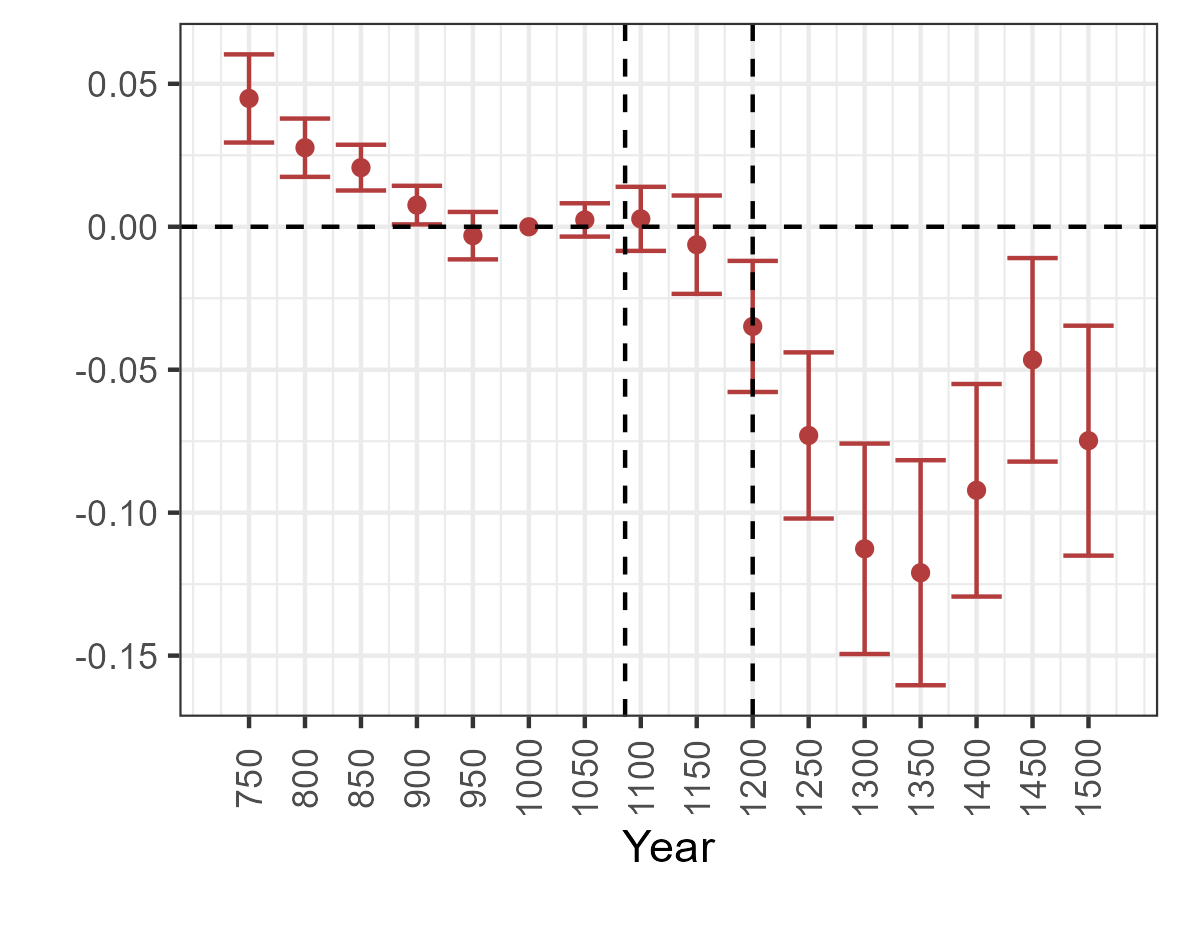
\includegraphics[width=\textwidth]{Plots/Regression_plots/arch_MA_coins_norm.png}
    \end{subfigure}
    \hfill
    \begin{subfigure}[b]{0.45\textwidth}
        \centering
        \caption{Coins: Dummy approach} \label{fig:arch1b_norm}
        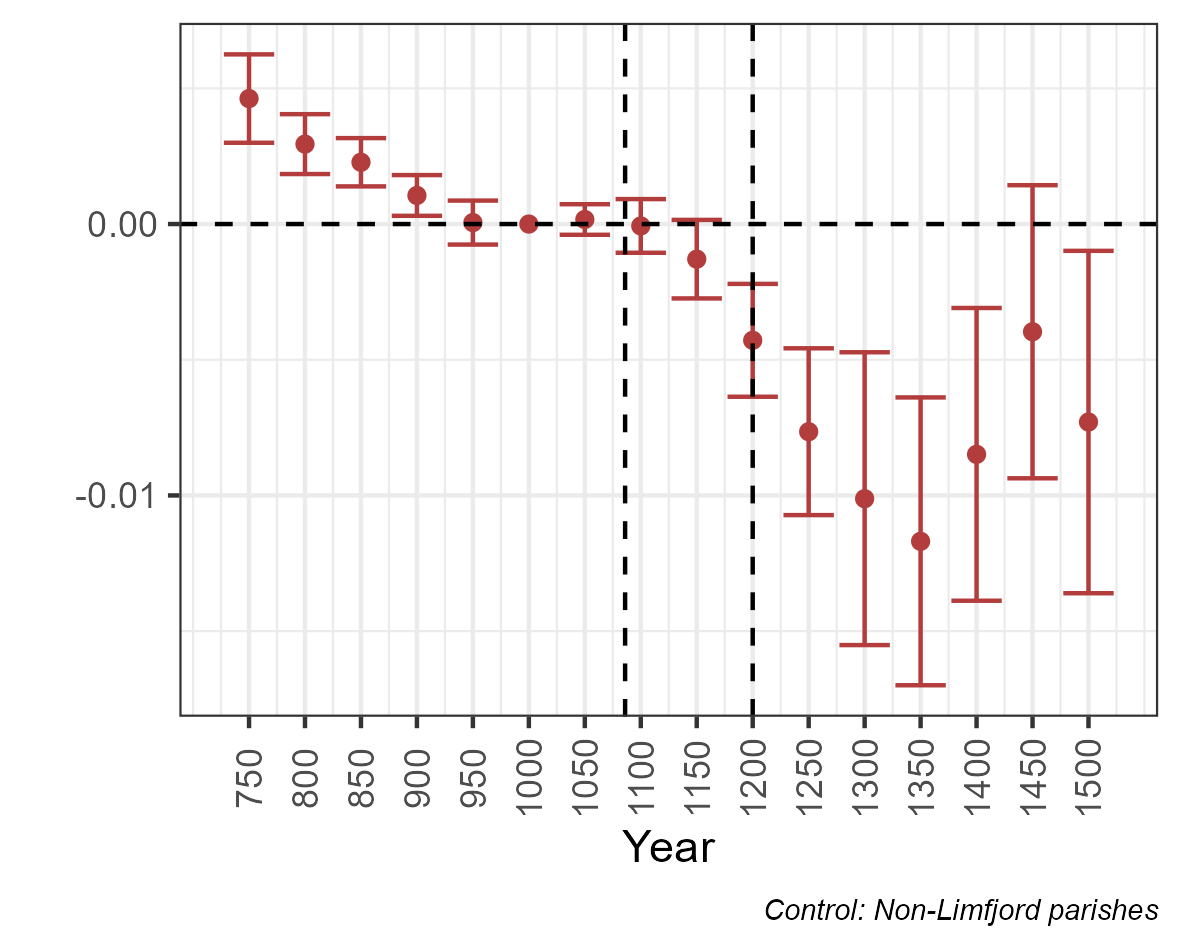
\includegraphics[width=\textwidth]{Plots/Regression_plots/arch_dummy_coins_norm.png}
    \end{subfigure}
    \vspace{0.45cm}
    \begin{subfigure}[b]{0.45\textwidth}
        \centering
        \caption{Buildings: Market access approach} \label{fig:arch1c_norm}
        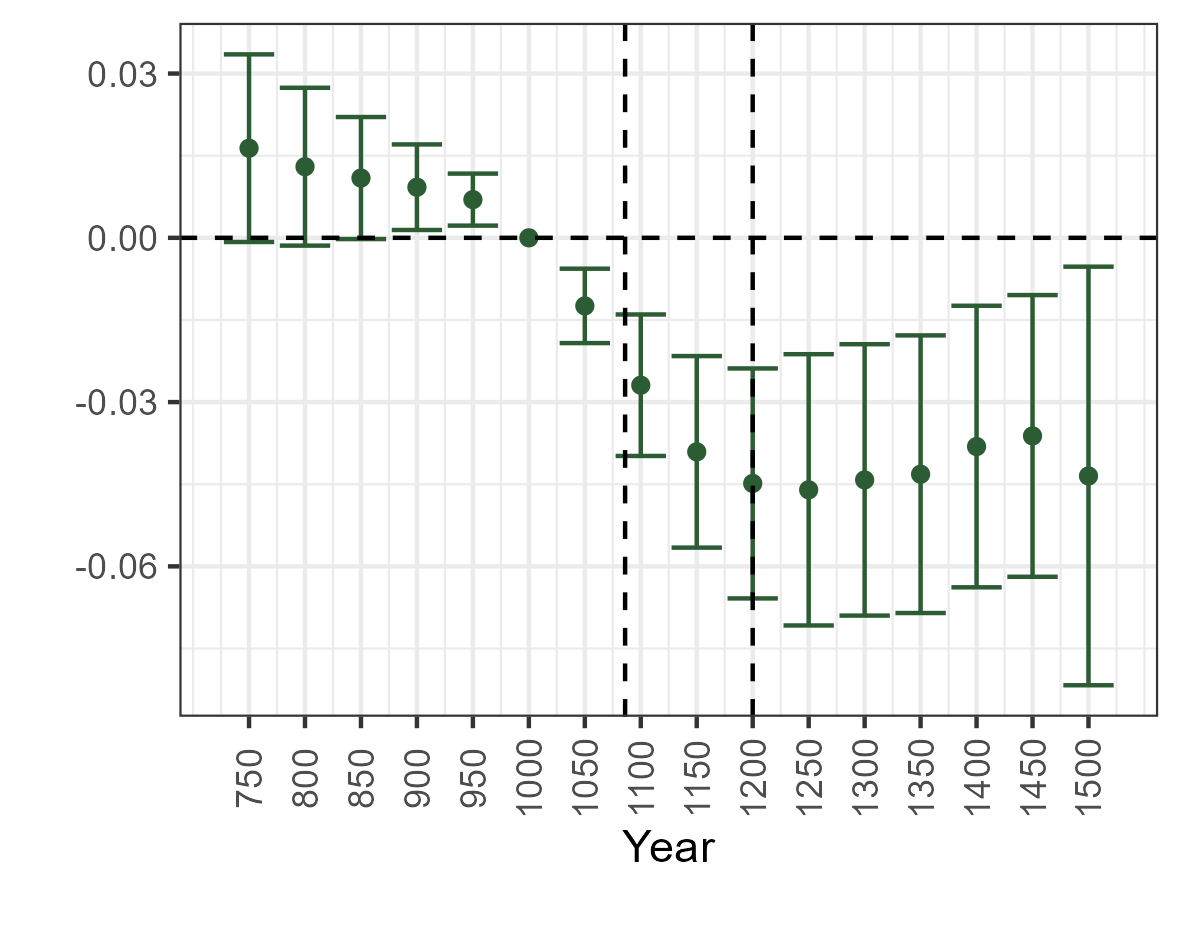
\includegraphics[width=\textwidth]{Plots/Regression_plots/arch_MA_buildings_norm.png}
    \end{subfigure}
    \hfill
    \begin{subfigure}[b]{0.45\textwidth}
        \centering
        \caption{Buildings: Dummy approach} \label{fig:arch1d_norm}
        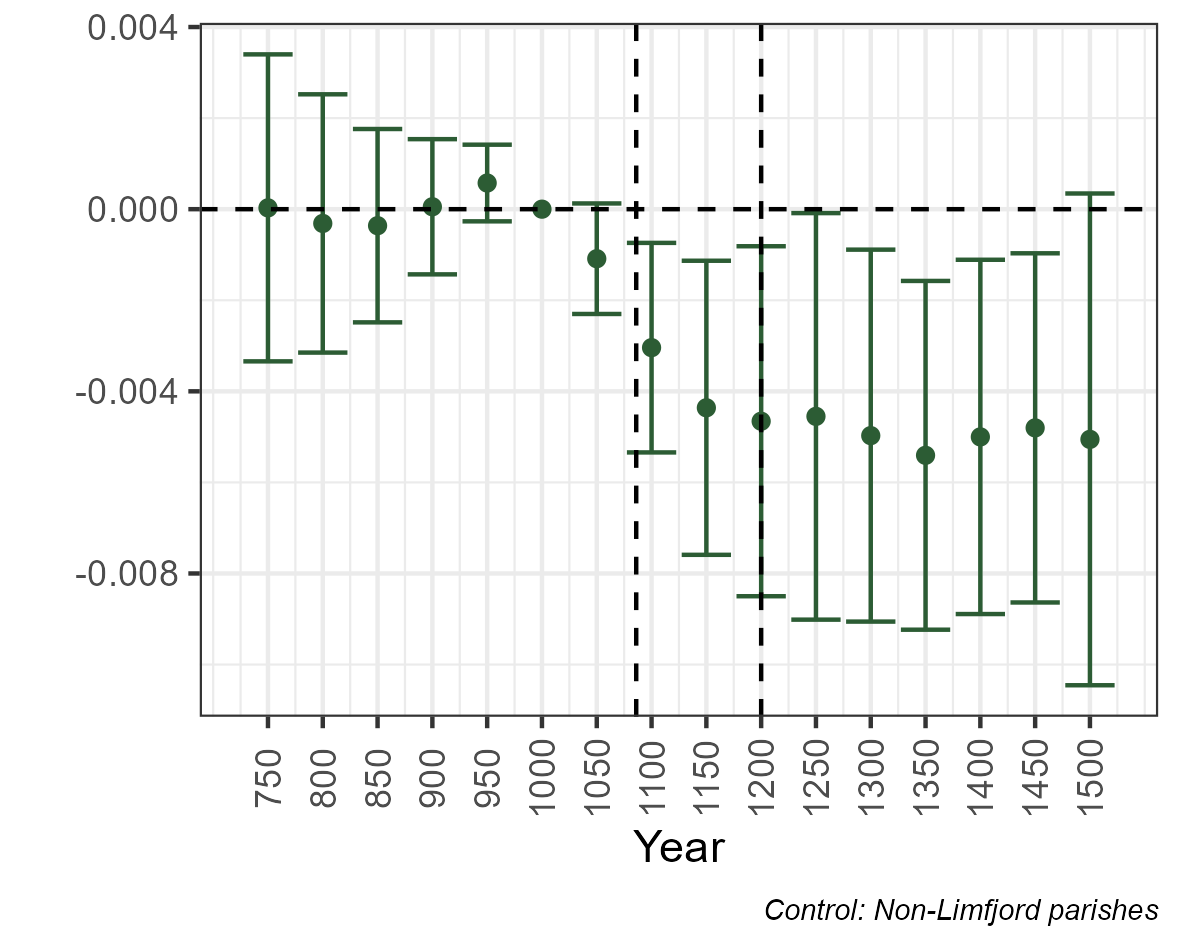
\includegraphics[width=\textwidth]{Plots/Regression_plots/arch_dummy_buildings_norm.png}
    \end{subfigure}
    \label{fig:arch_reg1}
\end{figure}


\begin{figure}
    \centering
    \caption{Distribution of parameter estimates in 1350  (full sample)}
    \begin{subfigure}[b]{0.45\textwidth}
        \centering
        \caption{Coins: Market access approach} \label{fig:distri_a_norm}
        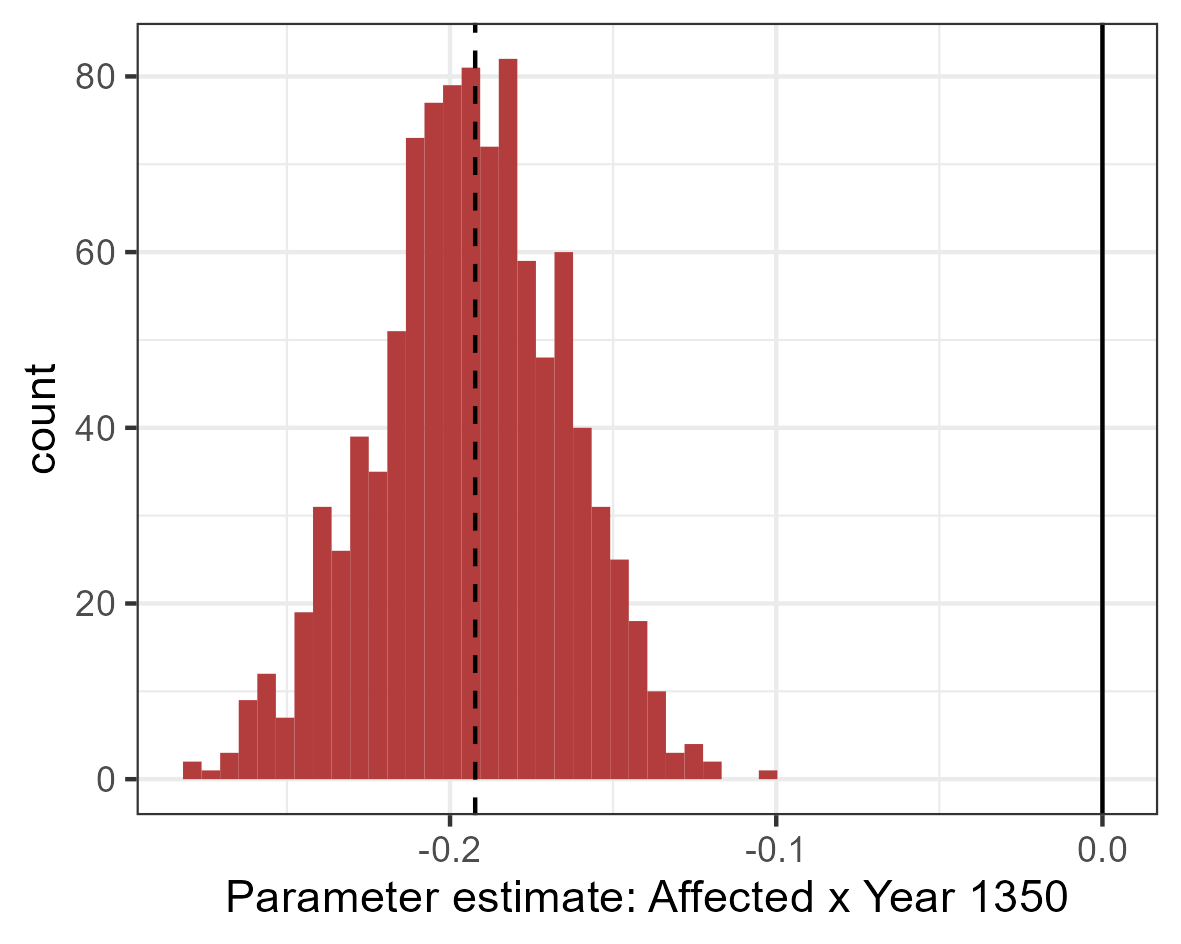
\includegraphics[width=\textwidth]{Plots/Regression_plots/arch_MA_coins_boot_norm.png}
    \end{subfigure}
    \hfill
    \begin{subfigure}[b]{0.45\textwidth}
        \centering
        \caption{Coins: Dummy approach} \label{fig:distri_b_norm}
        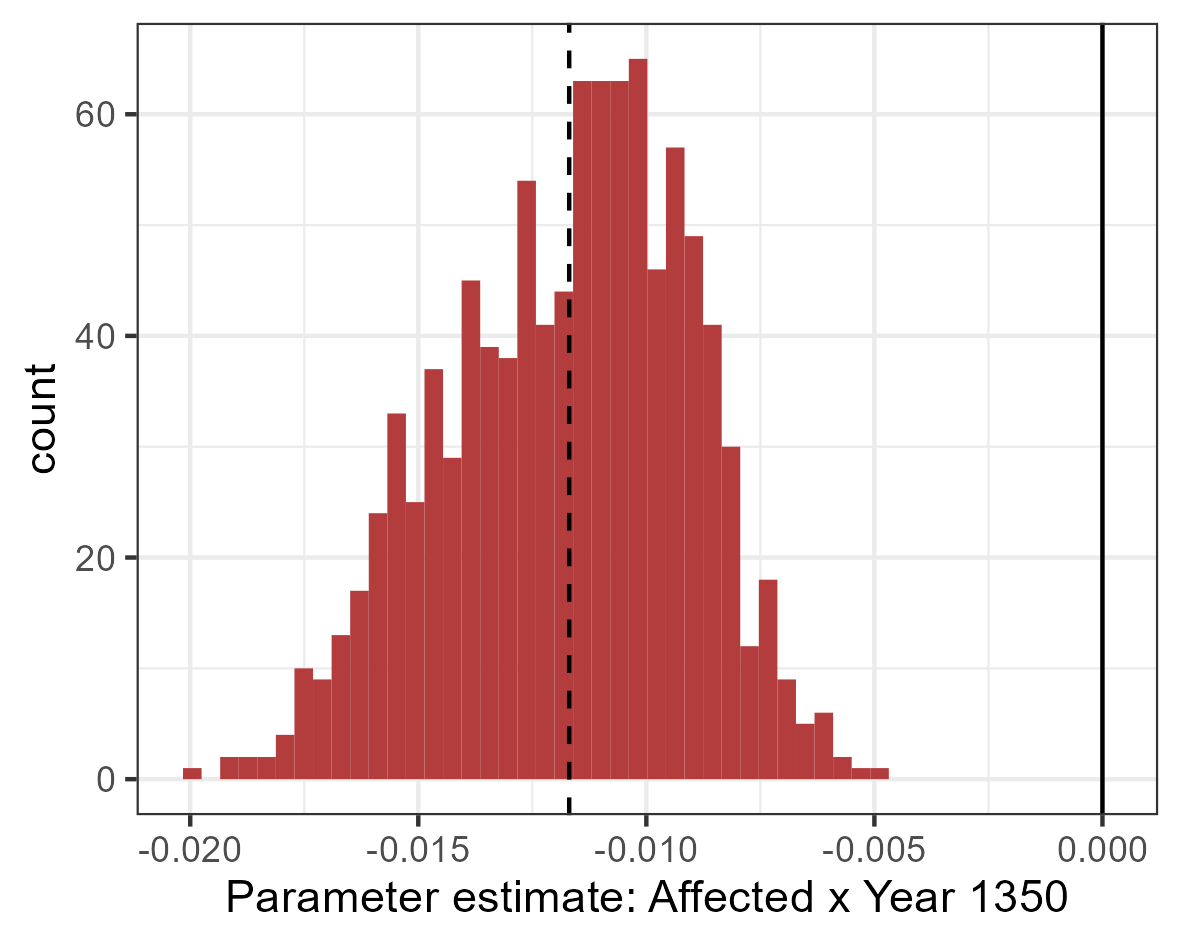
\includegraphics[width=\textwidth]{Plots/Regression_plots/arch_dummy_coins_boot_norm.png}
    \end{subfigure}
    \vspace{0.45cm}
    \begin{subfigure}[b]{0.45\textwidth}
        \centering
        \caption{Buildings: Market access approach} \label{fig:distri_c_norm}
        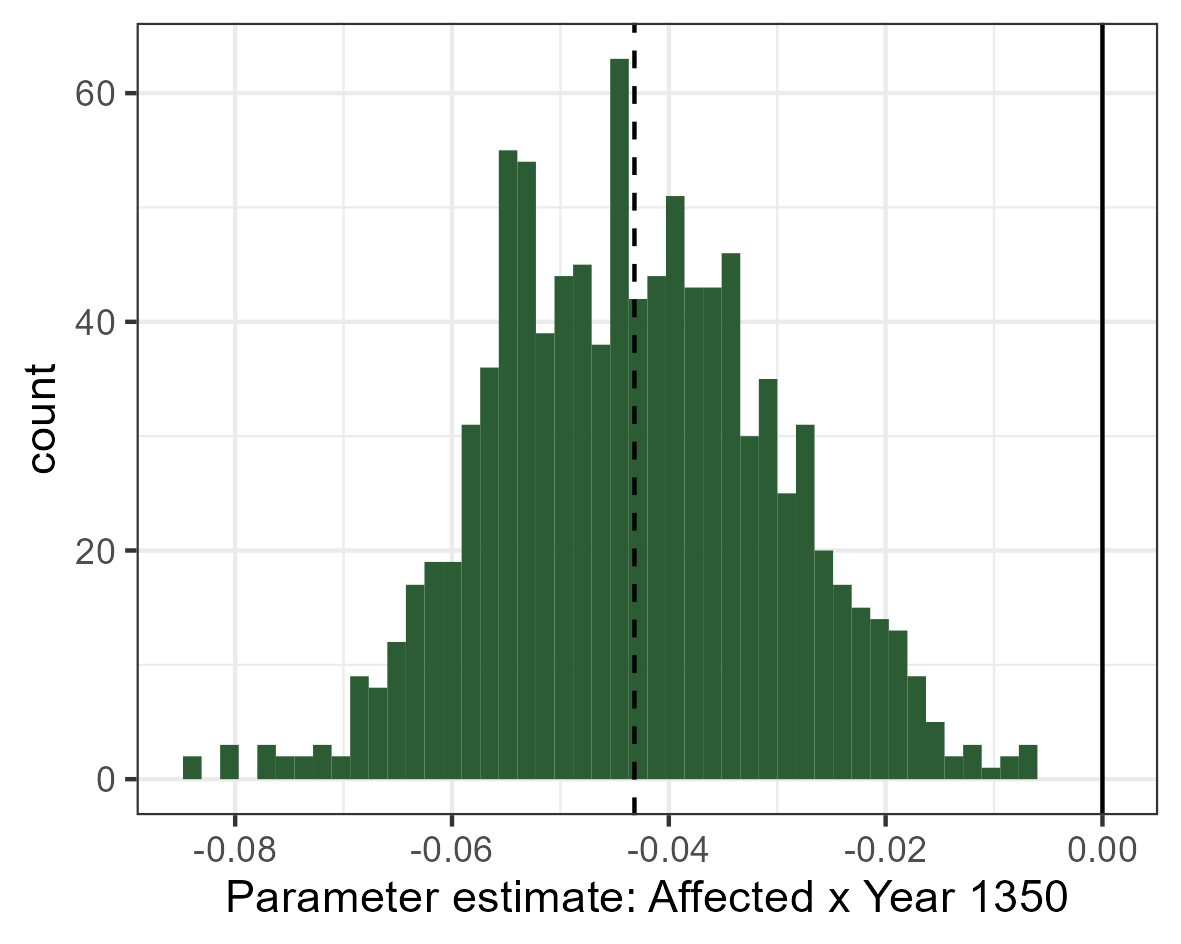
\includegraphics[width=\textwidth]{Plots/Regression_plots/arch_MA_buildings_boot_norm.png}
    \end{subfigure}
    \hfill
    \begin{subfigure}[b]{0.45\textwidth}
        \centering
        \caption{Buildings: Dummy approach} \label{fig:distri_d_norm}
        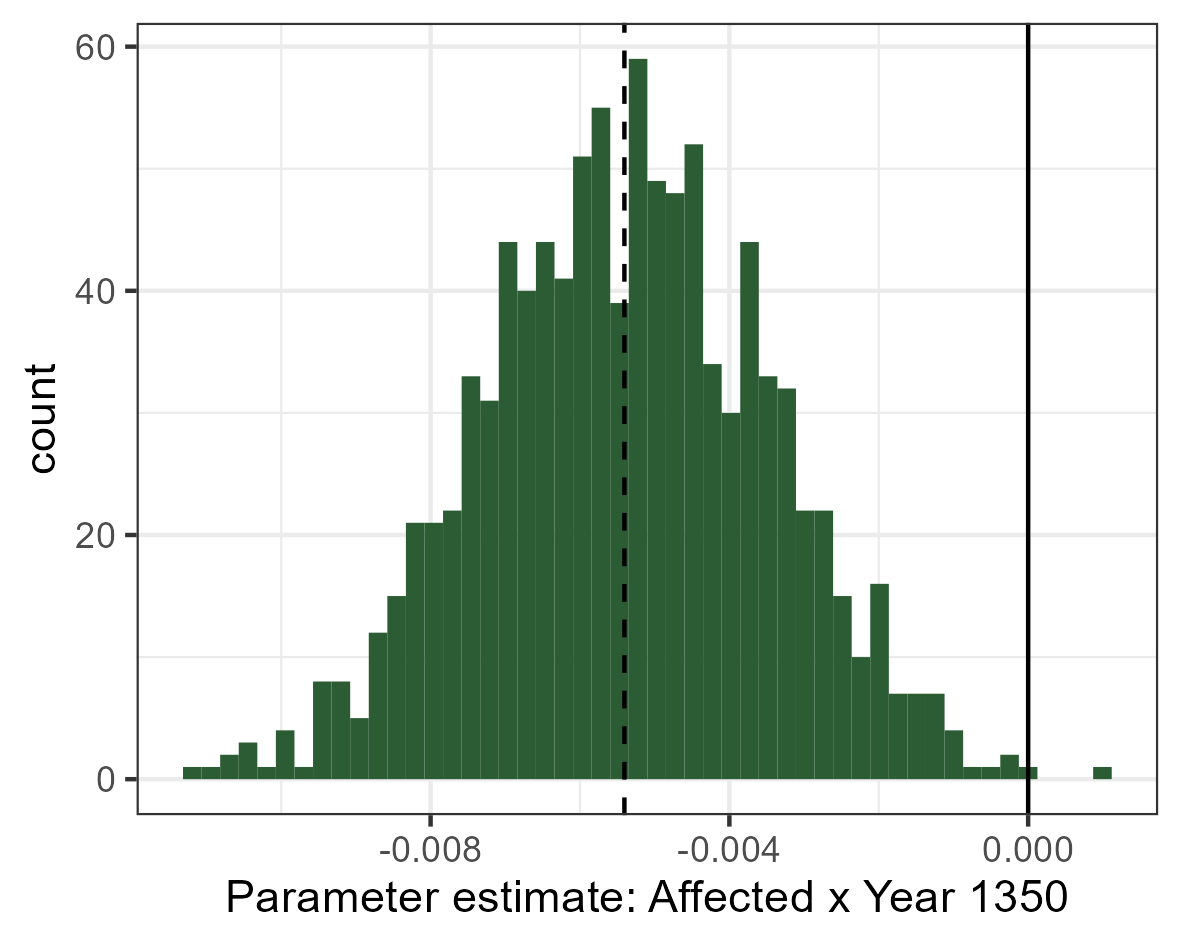
\includegraphics[width=\textwidth]{Plots/Regression_plots/arch_dummy_buildings_boot_norm.png}
    \end{subfigure}
    \label{fig:arch_reg_boot1}
\end{figure}


\begin{figure}
    \centering
    \caption{Archaelogical results (matched sample)}
    \begin{subfigure}[b]{0.45\textwidth}
        \centering
        \caption{Coins: Market access approach} \label{fig:arch1a_match_norm}
        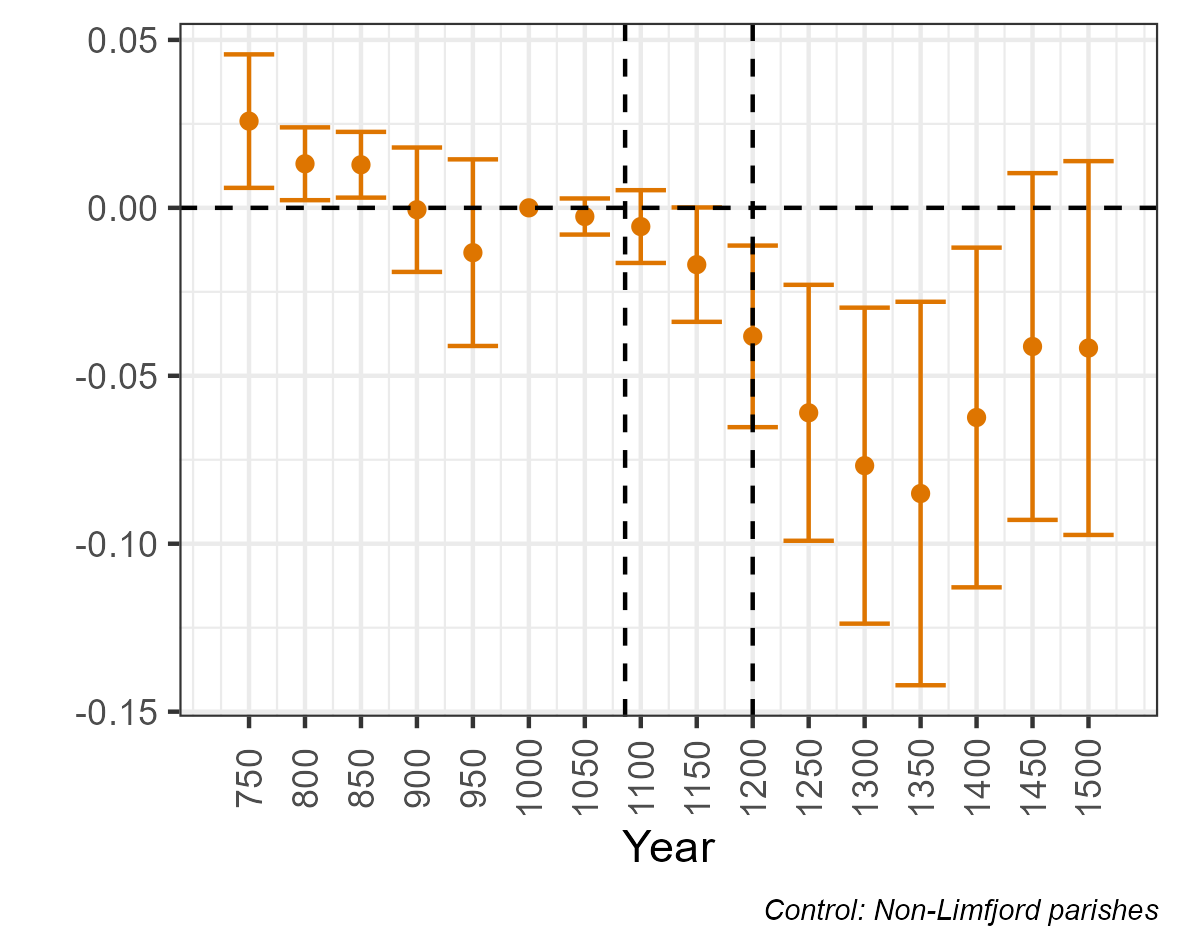
\includegraphics[width=\textwidth]{Plots/Regression_plots/arch_MA_coins_matched_norm.png}
    \end{subfigure}
    \hfill
    \begin{subfigure}[b]{0.45\textwidth}
        \centering
        \caption{Coins: Dummy approach} \label{fig:arch1b_match_norm}
        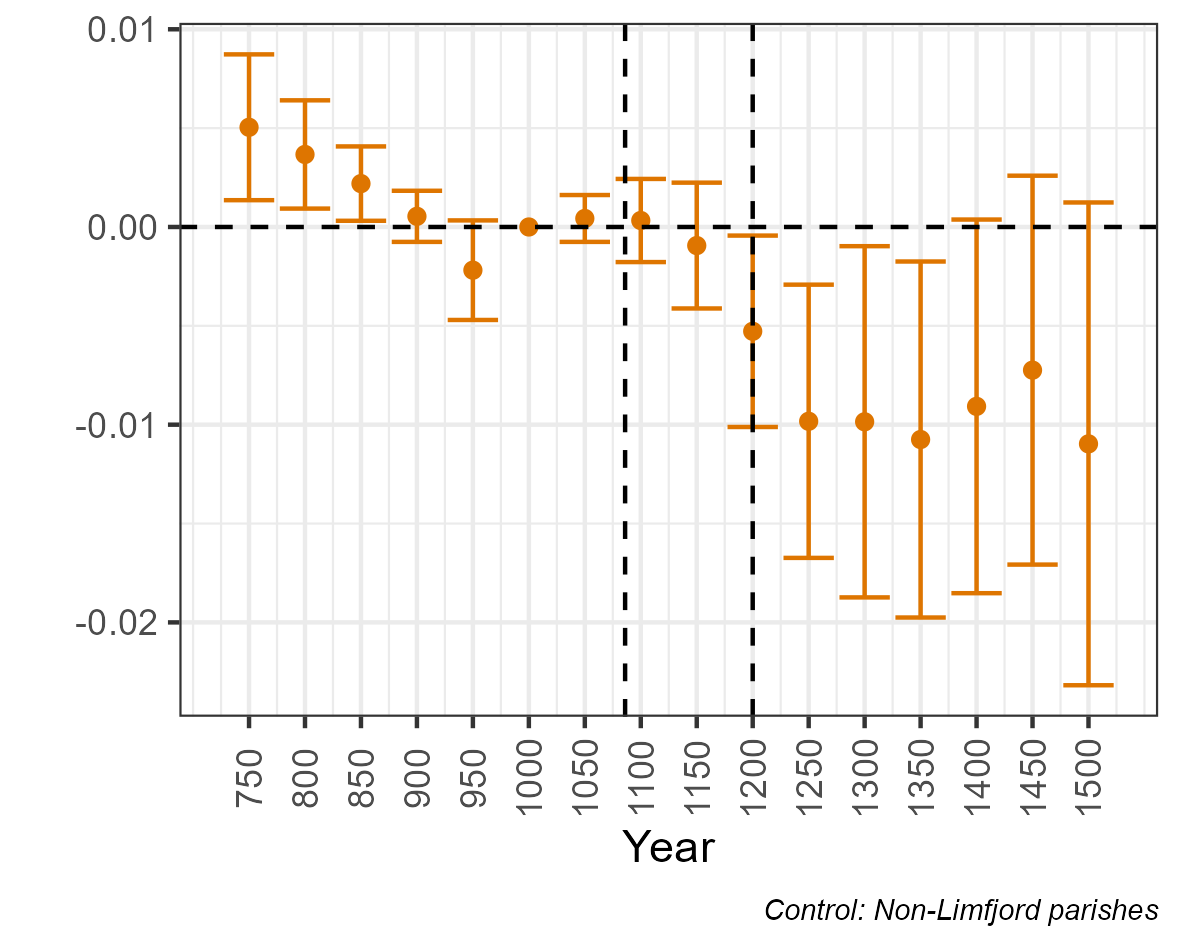
\includegraphics[width=\textwidth]{Plots/Regression_plots/arch_dummy_coins_matched_norm.png}
    \end{subfigure}
    \vspace{0.45cm}
    \begin{subfigure}[b]{0.45\textwidth}
        \centering
        \caption{Buildings: Market access approach} \label{fig:arch1c_match_norm}
        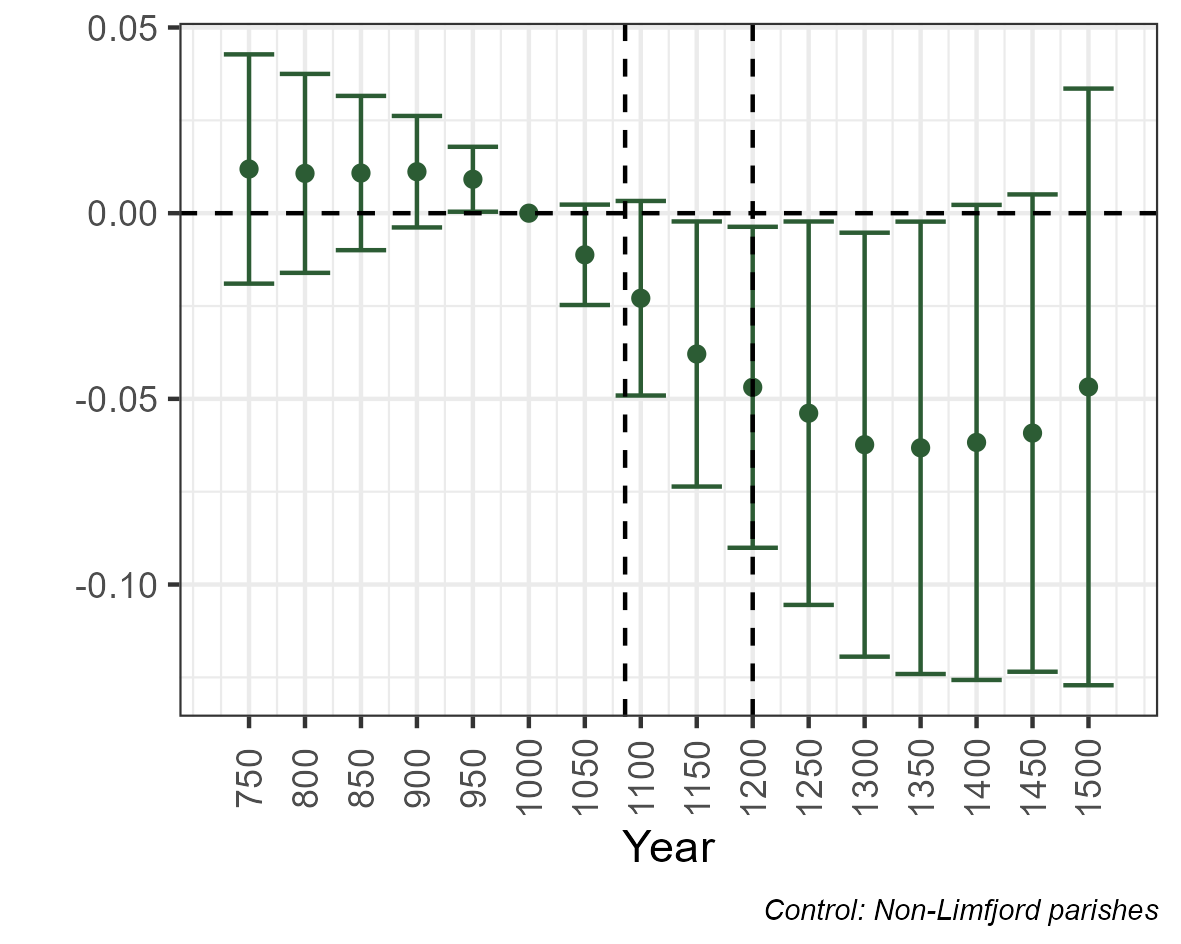
\includegraphics[width=\textwidth]{Plots/Regression_plots/arch_MA_buildings_matched_norm.png}
    \end{subfigure}
    \hfill
    \begin{subfigure}[b]{0.45\textwidth}
        \centering
        \caption{Buildings: Dummy approach} \label{fig:arch1d_match_norm}
        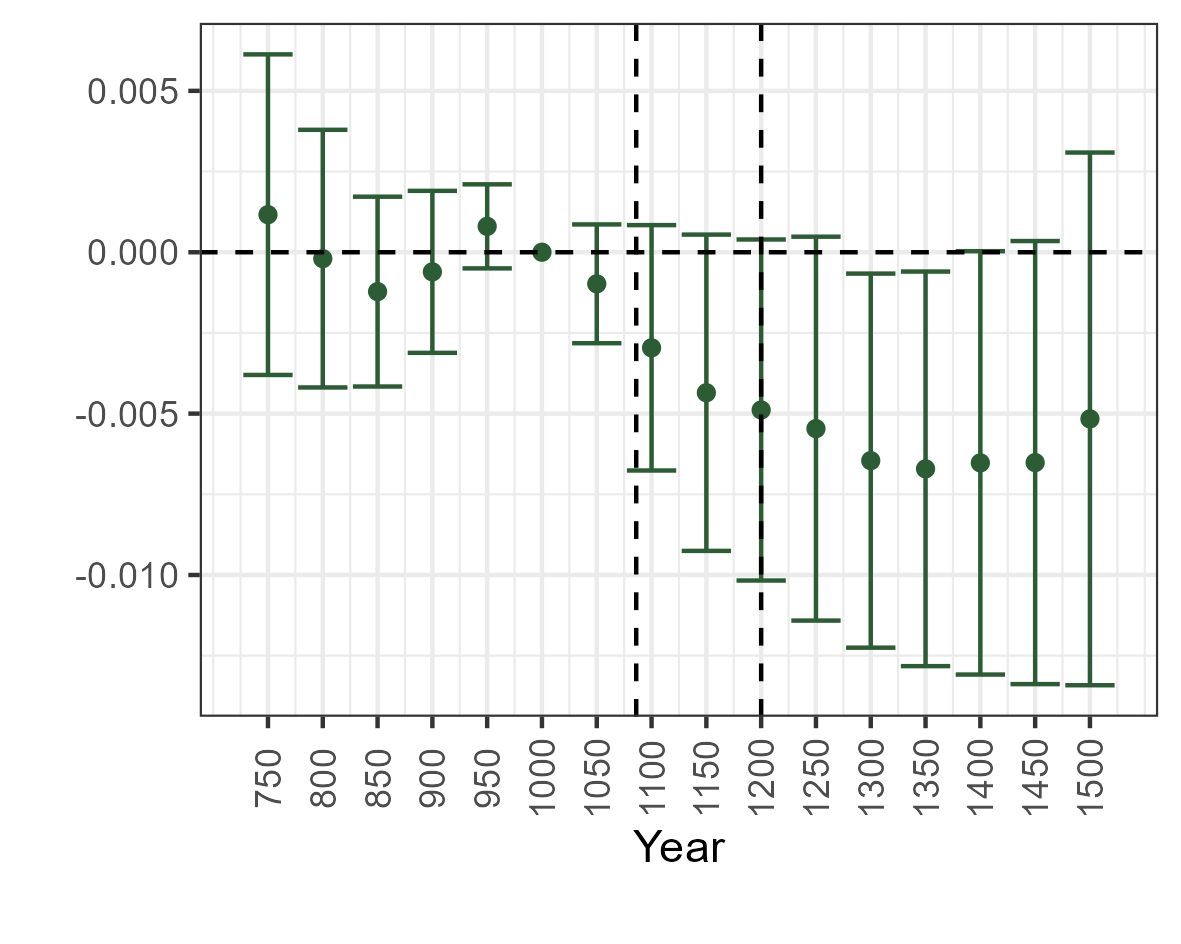
\includegraphics[width=\textwidth]{Plots/Regression_plots/arch_dummy_buildings_matched_norm.png}
    \end{subfigure}
    \label{fig:arch_reg2}
\end{figure}


\begin{figure}
    \centering
    \caption{Distribution of parameter estimates in 1350  (matched sample)}
    \begin{subfigure}[b]{0.45\textwidth}
        \centering
        \caption{Coins: Market access approach} \label{fig:distri_a_match_norm}
        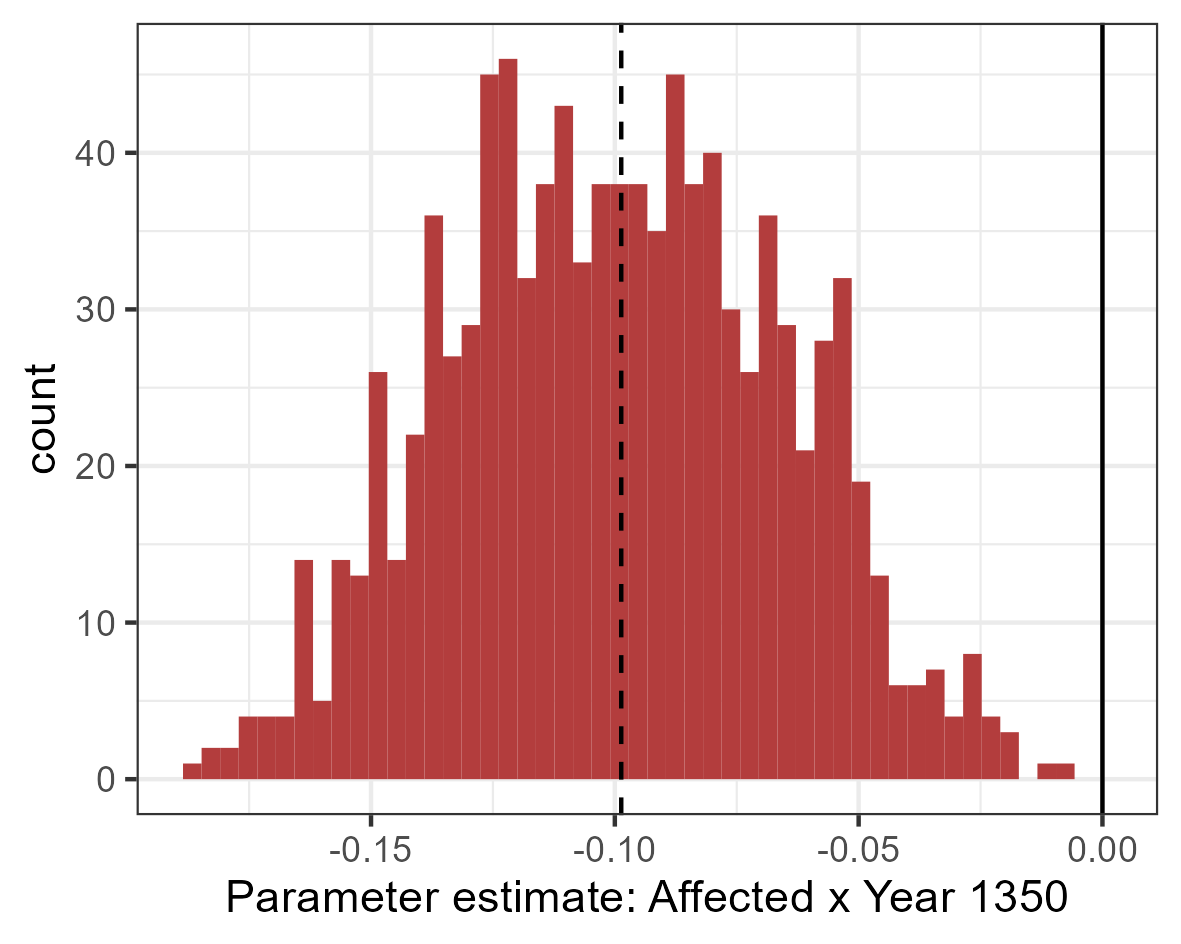
\includegraphics[width=\textwidth]{Plots/Regression_plots/arch_MA_coins_matched_boot_norm.png}
    \end{subfigure}
    \hfill
    \begin{subfigure}[b]{0.45\textwidth}
        \centering
        \caption{Coins: Dummy approach} \label{fig:distri_b_match_norm}
        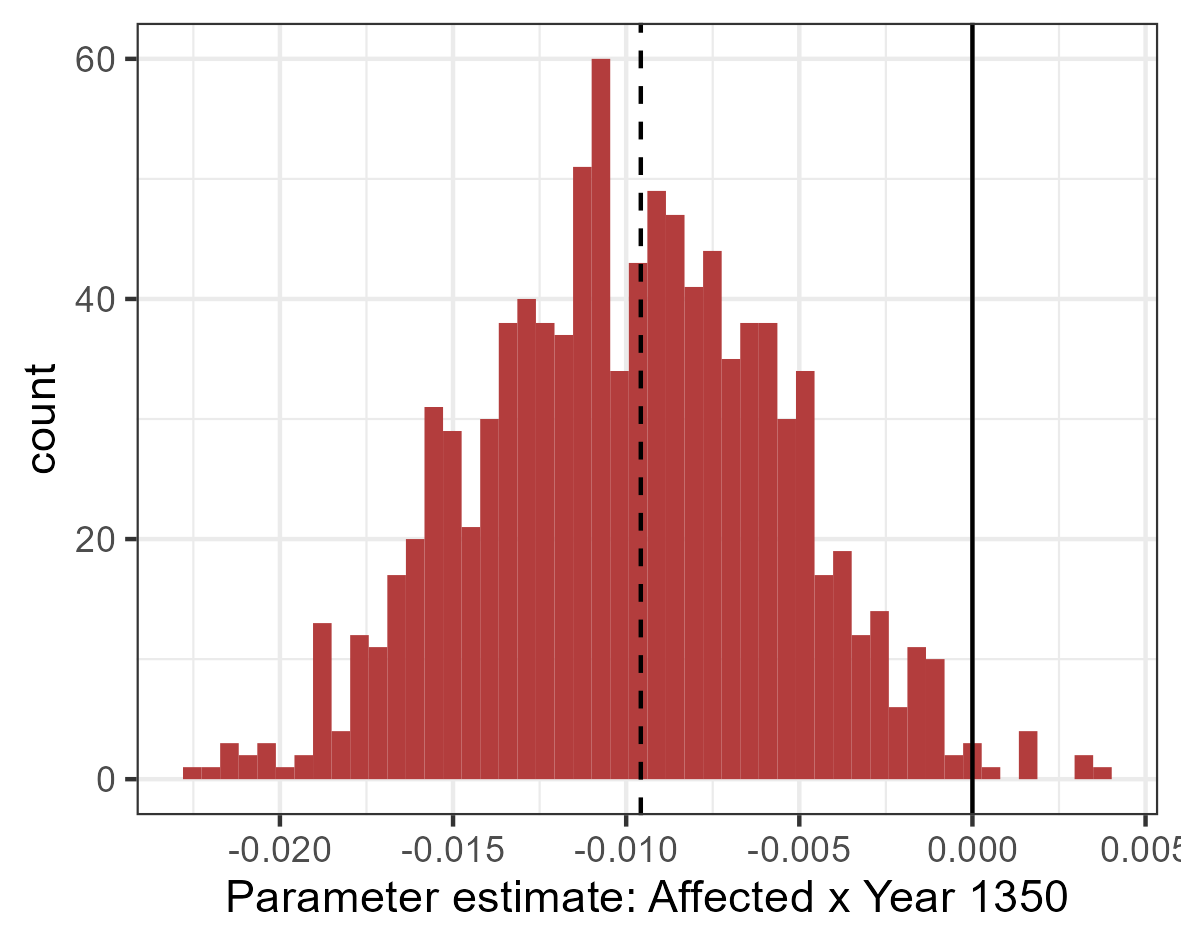
\includegraphics[width=\textwidth]{Plots/Regression_plots/arch_dummy_coins_matched_boot_norm.png}
    \end{subfigure}
    \vspace{0.45cm}
    \begin{subfigure}[b]{0.45\textwidth}
        \centering
        \caption{Buildings: Market access approach} \label{fig:distri_c_match_norm}
        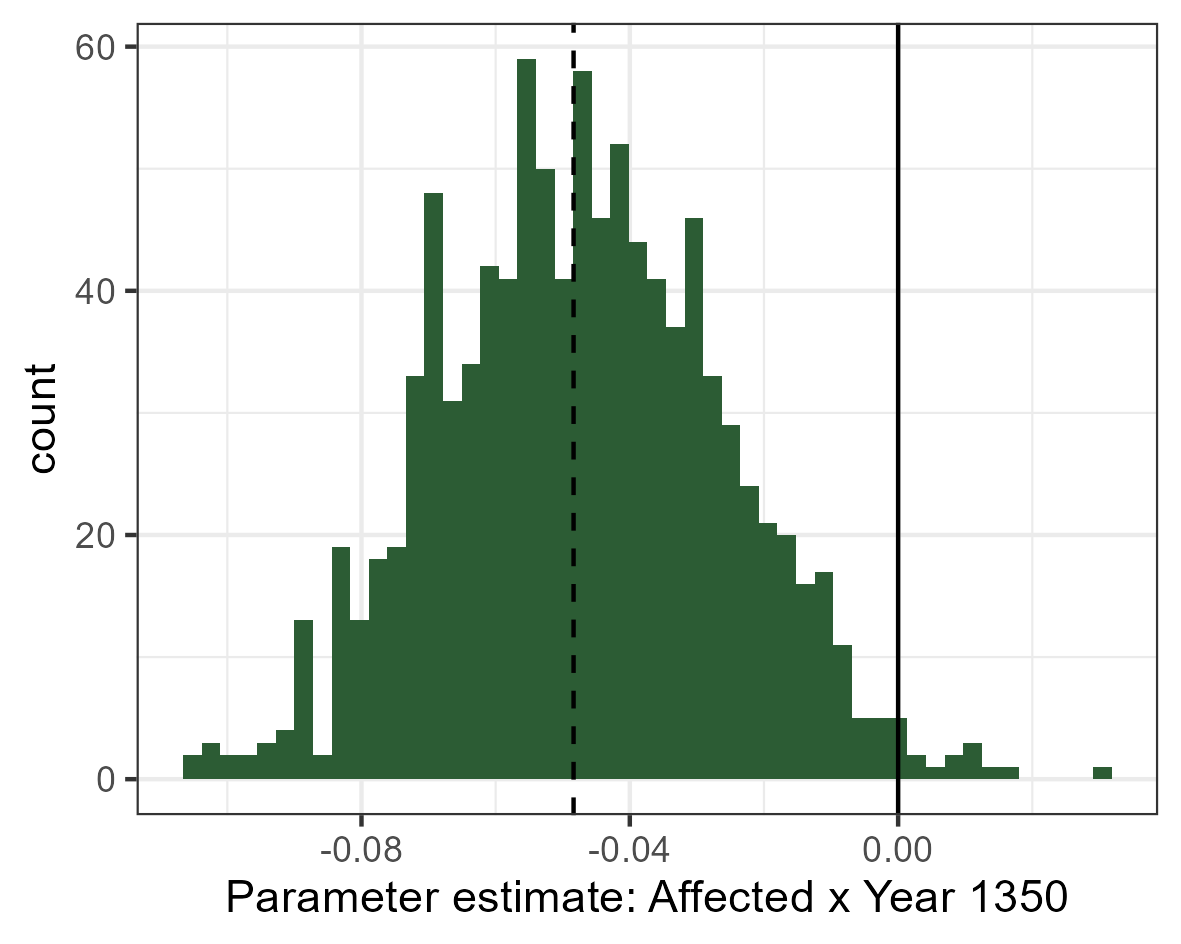
\includegraphics[width=\textwidth]{Plots/Regression_plots/arch_MA_buildings_matched_boot_norm.png}
    \end{subfigure}
    \hfill
    \begin{subfigure}[b]{0.45\textwidth}
        \centering
        \caption{Buildings: Dummy approach} \label{fig:distri_d_match_norm}
        \includegraphics[width=\textwidth]{Plots/Regression_plots/arch_dummy_buildings_matched_boot_norm.png}
    \end{subfigure}
    \label{fig:arch_reg_boot2}
\end{figure}






\end{document}



